\documentclass[12pt]{report}
\usepackage[pdftex]{graphicx}
\usepackage[margin=1.2in]{geometry}
\usepackage[utf8]{inputenc}

\usepackage{graphicx}
\graphicspath{{./images/}}

\usepackage{listings}
\newcommand\lstinputpath[1]{\lstset{inputpath=#1}}
\lstinputpath{codes}

\usepackage{xcolor}
\usepackage{titlesec}
 
\titleformat{\chapter}[display]
  {\normalfont\bfseries}{}{0pt}{\Huge}

\definecolor{codegreen}{rgb}{0,0.6,0}
\definecolor{codegray}{rgb}{0.5,0.5,0.5}
\definecolor{codepurple}{rgb}{0.58,0,0.82}
\definecolor{backcolour}{rgb}{0.95,0.95,0.92}

\lstdefinestyle{mystyle}{
    backgroundcolor=\color{backcolour},   
    commentstyle=\color{codegreen},
    keywordstyle=\color{magenta},
    numberstyle=\tiny\color{codegray},
    stringstyle=\color{codepurple},
    basicstyle=\ttfamily\footnotesize,
    breakatwhitespace=false,         
    breaklines=true,                 
    captionpos=b,                    
    keepspaces=true,                 
    numbers=left,                    
    numbersep=5pt,                  
    showspaces=false,                
    showstringspaces=false,
    showtabs=false,                  
    tabsize=2
}

\lstset{style=mystyle}

\usepackage{hyperref}
\hypersetup{
    colorlinks=true,
    linkcolor=blue,
    filecolor=magenta,      
    urlcolor=cyan,
}

\urlstyle{same}


\title{

    \begin{figure}
      \centering
      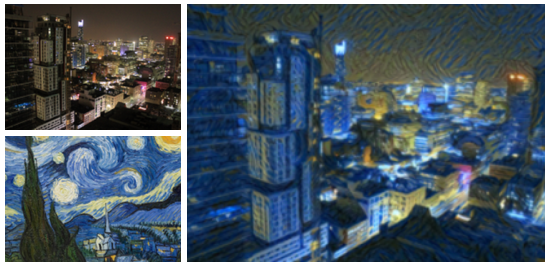
\includegraphics[scale=1]{cover.png}
    \end{figure}


    \textbf{Neural Network and Machine Learning}\\\large{Midterm Report for Summer of Science - 2020}
}
\author{Name: Sahasra Ranjan\\Mentor: Amitrajit Bhattacharjee}
\date{Roll no.: 190050102}











    \usepackage[breakable]{tcolorbox}
    \usepackage{parskip} % Stop auto-indenting (to mimic markdown behaviour)
    
    \usepackage{iftex}
    \ifPDFTeX
      \usepackage[T1]{fontenc}
      \usepackage{mathpazo}
    \else
      \usepackage{fontspec}
    \fi

    % Basic figure setup, for now with no caption control since it's done
    % automatically by Pandoc (which extracts ![](path) syntax from Markdown).
    \usepackage{graphicx}
    % Maintain compatibility with old templates. Remove in nbconvert 6.0
    \let\Oldincludegraphics\includegraphics
    % Ensure that by default, figures have no caption (until we provide a
    % proper Figure object with a Caption API and a way to capture that
    % in the conversion process - todo).
    \usepackage{caption}
    \DeclareCaptionFormat{nocaption}{}
    \captionsetup{format=nocaption,aboveskip=0pt,belowskip=0pt}

    \usepackage[Export]{adjustbox} % Used to constrain images to a maximum size
    \adjustboxset{max size={0.9\linewidth}{0.9\paperheight}}
    \usepackage{float}
    \floatplacement{figure}{H} % forces figures to be placed at the correct location
    \usepackage{xcolor} % Allow colors to be defined
    \usepackage{enumerate} % Needed for markdown enumerations to work
    \usepackage{geometry} % Used to adjust the document margins
    \usepackage{amsmath} % Equations
    \usepackage{amssymb} % Equations
    \usepackage{textcomp} % defines textquotesingle
    % Hack from http://tex.stackexchange.com/a/47451/13684:
    \AtBeginDocument{%
        \def\PYZsq{\textquotesingle}% Upright quotes in Pygmentized code
    }
    \usepackage{upquote} % Upright quotes for verbatim code
    \usepackage{eurosym} % defines \euro
    \usepackage[mathletters]{ucs} % Extended unicode (utf-8) support
    \usepackage{fancyvrb} % verbatim replacement that allows latex
    \usepackage{grffile} % extends the file name processing of package graphics 
                         % to support a larger range
    \makeatletter % fix for grffile with XeLaTeX
    \def\Gread@@xetex#1{%
      \IfFileExists{"\Gin@base".bb}%
      {\Gread@eps{\Gin@base.bb}}%
      {\Gread@@xetex@aux#1}%
    }
    \makeatother

    % The hyperref package gives us a pdf with properly built
    % internal navigation ('pdf bookmarks' for the table of contents,
    % internal cross-reference links, web links for URLs, etc.)
    \usepackage{hyperref}
    % The default LaTeX title has an obnoxious amount of whitespace. By default,
    % titling removes some of it. It also provides customization options.
    \usepackage{titling}
    \usepackage{longtable} % longtable support required by pandoc >1.10
    \usepackage{booktabs}  % table support for pandoc > 1.12.2
    \usepackage[inline]{enumitem} % IRkernel/repr support (it uses the enumerate* environment)
    \usepackage[normalem]{ulem} % ulem is needed to support strikethroughs (\sout)
                                % normalem makes italics be italics, not underlines
    \usepackage{mathrsfs}
    

    
    % Colors for the hyperref package
    \definecolor{urlcolor}{rgb}{0,.145,.698}
    \definecolor{linkcolor}{rgb}{.71,0.21,0.01}
    \definecolor{citecolor}{rgb}{.12,.54,.11}

    % ANSI colors
    \definecolor{ansi-black}{HTML}{3E424D}
    \definecolor{ansi-black-intense}{HTML}{282C36}
    \definecolor{ansi-red}{HTML}{E75C58}
    \definecolor{ansi-red-intense}{HTML}{B22B31}
    \definecolor{ansi-green}{HTML}{00A250}
    \definecolor{ansi-green-intense}{HTML}{007427}
    \definecolor{ansi-yellow}{HTML}{DDB62B}
    \definecolor{ansi-yellow-intense}{HTML}{B27D12}
    \definecolor{ansi-blue}{HTML}{208FFB}
    \definecolor{ansi-blue-intense}{HTML}{0065CA}
    \definecolor{ansi-magenta}{HTML}{D160C4}
    \definecolor{ansi-magenta-intense}{HTML}{A03196}
    \definecolor{ansi-cyan}{HTML}{60C6C8}
    \definecolor{ansi-cyan-intense}{HTML}{258F8F}
    \definecolor{ansi-white}{HTML}{C5C1B4}
    \definecolor{ansi-white-intense}{HTML}{A1A6B2}
    \definecolor{ansi-default-inverse-fg}{HTML}{FFFFFF}
    \definecolor{ansi-default-inverse-bg}{HTML}{000000}

    % commands and environments needed by pandoc snippets
    % extracted from the output of `pandoc -s`
    \providecommand{\tightlist}{%
      \setlength{\itemsep}{0pt}\setlength{\parskip}{0pt}}
    \DefineVerbatimEnvironment{Highlighting}{Verbatim}{commandchars=\\\{\}}
    % Add ',fontsize=\small' for more characters per line
    \newenvironment{Shaded}{}{}
    \newcommand{\KeywordTok}[1]{\textcolor[rgb]{0.00,0.44,0.13}{\textbf{{#1}}}}
    \newcommand{\DataTypeTok}[1]{\textcolor[rgb]{0.56,0.13,0.00}{{#1}}}
    \newcommand{\DecValTok}[1]{\textcolor[rgb]{0.25,0.63,0.44}{{#1}}}
    \newcommand{\BaseNTok}[1]{\textcolor[rgb]{0.25,0.63,0.44}{{#1}}}
    \newcommand{\FloatTok}[1]{\textcolor[rgb]{0.25,0.63,0.44}{{#1}}}
    \newcommand{\CharTok}[1]{\textcolor[rgb]{0.25,0.44,0.63}{{#1}}}
    \newcommand{\StringTok}[1]{\textcolor[rgb]{0.25,0.44,0.63}{{#1}}}
    \newcommand{\CommentTok}[1]{\textcolor[rgb]{0.38,0.63,0.69}{\textit{{#1}}}}
    \newcommand{\OtherTok}[1]{\textcolor[rgb]{0.00,0.44,0.13}{{#1}}}
    \newcommand{\AlertTok}[1]{\textcolor[rgb]{1.00,0.00,0.00}{\textbf{{#1}}}}
    \newcommand{\FunctionTok}[1]{\textcolor[rgb]{0.02,0.16,0.49}{{#1}}}
    \newcommand{\RegionMarkerTok}[1]{{#1}}
    \newcommand{\ErrorTok}[1]{\textcolor[rgb]{1.00,0.00,0.00}{\textbf{{#1}}}}
    \newcommand{\NormalTok}[1]{{#1}}
    
    % Additional commands for more recent versions of Pandoc
    \newcommand{\ConstantTok}[1]{\textcolor[rgb]{0.53,0.00,0.00}{{#1}}}
    \newcommand{\SpecialCharTok}[1]{\textcolor[rgb]{0.25,0.44,0.63}{{#1}}}
    \newcommand{\VerbatimStringTok}[1]{\textcolor[rgb]{0.25,0.44,0.63}{{#1}}}
    \newcommand{\SpecialStringTok}[1]{\textcolor[rgb]{0.73,0.40,0.53}{{#1}}}
    \newcommand{\ImportTok}[1]{{#1}}
    \newcommand{\DocumentationTok}[1]{\textcolor[rgb]{0.73,0.13,0.13}{\textit{{#1}}}}
    \newcommand{\AnnotationTok}[1]{\textcolor[rgb]{0.38,0.63,0.69}{\textbf{\textit{{#1}}}}}
    \newcommand{\CommentVarTok}[1]{\textcolor[rgb]{0.38,0.63,0.69}{\textbf{\textit{{#1}}}}}
    \newcommand{\VariableTok}[1]{\textcolor[rgb]{0.10,0.09,0.49}{{#1}}}
    \newcommand{\ControlFlowTok}[1]{\textcolor[rgb]{0.00,0.44,0.13}{\textbf{{#1}}}}
    \newcommand{\OperatorTok}[1]{\textcolor[rgb]{0.40,0.40,0.40}{{#1}}}
    \newcommand{\BuiltInTok}[1]{{#1}}
    \newcommand{\ExtensionTok}[1]{{#1}}
    \newcommand{\PreprocessorTok}[1]{\textcolor[rgb]{0.74,0.48,0.00}{{#1}}}
    \newcommand{\AttributeTok}[1]{\textcolor[rgb]{0.49,0.56,0.16}{{#1}}}
    \newcommand{\InformationTok}[1]{\textcolor[rgb]{0.38,0.63,0.69}{\textbf{\textit{{#1}}}}}
    \newcommand{\WarningTok}[1]{\textcolor[rgb]{0.38,0.63,0.69}{\textbf{\textit{{#1}}}}}
    
    
    % Define a nice break command that doesn't care if a line doesn't already
    % exist.
    \def\br{\hspace*{\fill} \\* }
    % Math Jax compatibility definitions
    \def\gt{>}
    \def\lt{<}
    \let\Oldtex\TeX
    \let\Oldlatex\LaTeX
    \renewcommand{\TeX}{\textrm{\Oldtex}}
    \renewcommand{\LaTeX}{\textrm{\Oldlatex}}
    % Document parameters  
    
    
    
    
% Pygments definitions
\makeatletter
\def\PY@reset{\let\PY@it=\relax \let\PY@bf=\relax%
    \let\PY@ul=\relax \let\PY@tc=\relax%
    \let\PY@bc=\relax \let\PY@ff=\relax}
\def\PY@tok#1{\csname PY@tok@#1\endcsname}
\def\PY@toks#1+{\ifx\relax#1\empty\else%
    \PY@tok{#1}\expandafter\PY@toks\fi}
\def\PY@do#1{\PY@bc{\PY@tc{\PY@ul{%
    \PY@it{\PY@bf{\PY@ff{#1}}}}}}}
\def\PY#1#2{\PY@reset\PY@toks#1+\relax+\PY@do{#2}}

\expandafter\def\csname PY@tok@w\endcsname{\def\PY@tc##1{\textcolor[rgb]{0.73,0.73,0.73}{##1}}}
\expandafter\def\csname PY@tok@c\endcsname{\let\PY@it=\textit\def\PY@tc##1{\textcolor[rgb]{0.25,0.50,0.50}{##1}}}
\expandafter\def\csname PY@tok@cp\endcsname{\def\PY@tc##1{\textcolor[rgb]{0.74,0.48,0.00}{##1}}}
\expandafter\def\csname PY@tok@k\endcsname{\let\PY@bf=\textbf\def\PY@tc##1{\textcolor[rgb]{0.00,0.50,0.00}{##1}}}
\expandafter\def\csname PY@tok@kp\endcsname{\def\PY@tc##1{\textcolor[rgb]{0.00,0.50,0.00}{##1}}}
\expandafter\def\csname PY@tok@kt\endcsname{\def\PY@tc##1{\textcolor[rgb]{0.69,0.00,0.25}{##1}}}
\expandafter\def\csname PY@tok@o\endcsname{\def\PY@tc##1{\textcolor[rgb]{0.40,0.40,0.40}{##1}}}
\expandafter\def\csname PY@tok@ow\endcsname{\let\PY@bf=\textbf\def\PY@tc##1{\textcolor[rgb]{0.67,0.13,1.00}{##1}}}
\expandafter\def\csname PY@tok@nb\endcsname{\def\PY@tc##1{\textcolor[rgb]{0.00,0.50,0.00}{##1}}}
\expandafter\def\csname PY@tok@nf\endcsname{\def\PY@tc##1{\textcolor[rgb]{0.00,0.00,1.00}{##1}}}
\expandafter\def\csname PY@tok@nc\endcsname{\let\PY@bf=\textbf\def\PY@tc##1{\textcolor[rgb]{0.00,0.00,1.00}{##1}}}
\expandafter\def\csname PY@tok@nn\endcsname{\let\PY@bf=\textbf\def\PY@tc##1{\textcolor[rgb]{0.00,0.00,1.00}{##1}}}
\expandafter\def\csname PY@tok@ne\endcsname{\let\PY@bf=\textbf\def\PY@tc##1{\textcolor[rgb]{0.82,0.25,0.23}{##1}}}
\expandafter\def\csname PY@tok@nv\endcsname{\def\PY@tc##1{\textcolor[rgb]{0.10,0.09,0.49}{##1}}}
\expandafter\def\csname PY@tok@no\endcsname{\def\PY@tc##1{\textcolor[rgb]{0.53,0.00,0.00}{##1}}}
\expandafter\def\csname PY@tok@nl\endcsname{\def\PY@tc##1{\textcolor[rgb]{0.63,0.63,0.00}{##1}}}
\expandafter\def\csname PY@tok@ni\endcsname{\let\PY@bf=\textbf\def\PY@tc##1{\textcolor[rgb]{0.60,0.60,0.60}{##1}}}
\expandafter\def\csname PY@tok@na\endcsname{\def\PY@tc##1{\textcolor[rgb]{0.49,0.56,0.16}{##1}}}
\expandafter\def\csname PY@tok@nt\endcsname{\let\PY@bf=\textbf\def\PY@tc##1{\textcolor[rgb]{0.00,0.50,0.00}{##1}}}
\expandafter\def\csname PY@tok@nd\endcsname{\def\PY@tc##1{\textcolor[rgb]{0.67,0.13,1.00}{##1}}}
\expandafter\def\csname PY@tok@s\endcsname{\def\PY@tc##1{\textcolor[rgb]{0.73,0.13,0.13}{##1}}}
\expandafter\def\csname PY@tok@sd\endcsname{\let\PY@it=\textit\def\PY@tc##1{\textcolor[rgb]{0.73,0.13,0.13}{##1}}}
\expandafter\def\csname PY@tok@si\endcsname{\let\PY@bf=\textbf\def\PY@tc##1{\textcolor[rgb]{0.73,0.40,0.53}{##1}}}
\expandafter\def\csname PY@tok@se\endcsname{\let\PY@bf=\textbf\def\PY@tc##1{\textcolor[rgb]{0.73,0.40,0.13}{##1}}}
\expandafter\def\csname PY@tok@sr\endcsname{\def\PY@tc##1{\textcolor[rgb]{0.73,0.40,0.53}{##1}}}
\expandafter\def\csname PY@tok@ss\endcsname{\def\PY@tc##1{\textcolor[rgb]{0.10,0.09,0.49}{##1}}}
\expandafter\def\csname PY@tok@sx\endcsname{\def\PY@tc##1{\textcolor[rgb]{0.00,0.50,0.00}{##1}}}
\expandafter\def\csname PY@tok@m\endcsname{\def\PY@tc##1{\textcolor[rgb]{0.40,0.40,0.40}{##1}}}
\expandafter\def\csname PY@tok@gh\endcsname{\let\PY@bf=\textbf\def\PY@tc##1{\textcolor[rgb]{0.00,0.00,0.50}{##1}}}
\expandafter\def\csname PY@tok@gu\endcsname{\let\PY@bf=\textbf\def\PY@tc##1{\textcolor[rgb]{0.50,0.00,0.50}{##1}}}
\expandafter\def\csname PY@tok@gd\endcsname{\def\PY@tc##1{\textcolor[rgb]{0.63,0.00,0.00}{##1}}}
\expandafter\def\csname PY@tok@gi\endcsname{\def\PY@tc##1{\textcolor[rgb]{0.00,0.63,0.00}{##1}}}
\expandafter\def\csname PY@tok@gr\endcsname{\def\PY@tc##1{\textcolor[rgb]{1.00,0.00,0.00}{##1}}}
\expandafter\def\csname PY@tok@ge\endcsname{\let\PY@it=\textit}
\expandafter\def\csname PY@tok@gs\endcsname{\let\PY@bf=\textbf}
\expandafter\def\csname PY@tok@gp\endcsname{\let\PY@bf=\textbf\def\PY@tc##1{\textcolor[rgb]{0.00,0.00,0.50}{##1}}}
\expandafter\def\csname PY@tok@go\endcsname{\def\PY@tc##1{\textcolor[rgb]{0.53,0.53,0.53}{##1}}}
\expandafter\def\csname PY@tok@gt\endcsname{\def\PY@tc##1{\textcolor[rgb]{0.00,0.27,0.87}{##1}}}
\expandafter\def\csname PY@tok@err\endcsname{\def\PY@bc##1{\setlength{\fboxsep}{0pt}\fcolorbox[rgb]{1.00,0.00,0.00}{1,1,1}{\strut ##1}}}
\expandafter\def\csname PY@tok@kc\endcsname{\let\PY@bf=\textbf\def\PY@tc##1{\textcolor[rgb]{0.00,0.50,0.00}{##1}}}
\expandafter\def\csname PY@tok@kd\endcsname{\let\PY@bf=\textbf\def\PY@tc##1{\textcolor[rgb]{0.00,0.50,0.00}{##1}}}
\expandafter\def\csname PY@tok@kn\endcsname{\let\PY@bf=\textbf\def\PY@tc##1{\textcolor[rgb]{0.00,0.50,0.00}{##1}}}
\expandafter\def\csname PY@tok@kr\endcsname{\let\PY@bf=\textbf\def\PY@tc##1{\textcolor[rgb]{0.00,0.50,0.00}{##1}}}
\expandafter\def\csname PY@tok@bp\endcsname{\def\PY@tc##1{\textcolor[rgb]{0.00,0.50,0.00}{##1}}}
\expandafter\def\csname PY@tok@fm\endcsname{\def\PY@tc##1{\textcolor[rgb]{0.00,0.00,1.00}{##1}}}
\expandafter\def\csname PY@tok@vc\endcsname{\def\PY@tc##1{\textcolor[rgb]{0.10,0.09,0.49}{##1}}}
\expandafter\def\csname PY@tok@vg\endcsname{\def\PY@tc##1{\textcolor[rgb]{0.10,0.09,0.49}{##1}}}
\expandafter\def\csname PY@tok@vi\endcsname{\def\PY@tc##1{\textcolor[rgb]{0.10,0.09,0.49}{##1}}}
\expandafter\def\csname PY@tok@vm\endcsname{\def\PY@tc##1{\textcolor[rgb]{0.10,0.09,0.49}{##1}}}
\expandafter\def\csname PY@tok@sa\endcsname{\def\PY@tc##1{\textcolor[rgb]{0.73,0.13,0.13}{##1}}}
\expandafter\def\csname PY@tok@sb\endcsname{\def\PY@tc##1{\textcolor[rgb]{0.73,0.13,0.13}{##1}}}
\expandafter\def\csname PY@tok@sc\endcsname{\def\PY@tc##1{\textcolor[rgb]{0.73,0.13,0.13}{##1}}}
\expandafter\def\csname PY@tok@dl\endcsname{\def\PY@tc##1{\textcolor[rgb]{0.73,0.13,0.13}{##1}}}
\expandafter\def\csname PY@tok@s2\endcsname{\def\PY@tc##1{\textcolor[rgb]{0.73,0.13,0.13}{##1}}}
\expandafter\def\csname PY@tok@sh\endcsname{\def\PY@tc##1{\textcolor[rgb]{0.73,0.13,0.13}{##1}}}
\expandafter\def\csname PY@tok@s1\endcsname{\def\PY@tc##1{\textcolor[rgb]{0.73,0.13,0.13}{##1}}}
\expandafter\def\csname PY@tok@mb\endcsname{\def\PY@tc##1{\textcolor[rgb]{0.40,0.40,0.40}{##1}}}
\expandafter\def\csname PY@tok@mf\endcsname{\def\PY@tc##1{\textcolor[rgb]{0.40,0.40,0.40}{##1}}}
\expandafter\def\csname PY@tok@mh\endcsname{\def\PY@tc##1{\textcolor[rgb]{0.40,0.40,0.40}{##1}}}
\expandafter\def\csname PY@tok@mi\endcsname{\def\PY@tc##1{\textcolor[rgb]{0.40,0.40,0.40}{##1}}}
\expandafter\def\csname PY@tok@il\endcsname{\def\PY@tc##1{\textcolor[rgb]{0.40,0.40,0.40}{##1}}}
\expandafter\def\csname PY@tok@mo\endcsname{\def\PY@tc##1{\textcolor[rgb]{0.40,0.40,0.40}{##1}}}
\expandafter\def\csname PY@tok@ch\endcsname{\let\PY@it=\textit\def\PY@tc##1{\textcolor[rgb]{0.25,0.50,0.50}{##1}}}
\expandafter\def\csname PY@tok@cm\endcsname{\let\PY@it=\textit\def\PY@tc##1{\textcolor[rgb]{0.25,0.50,0.50}{##1}}}
\expandafter\def\csname PY@tok@cpf\endcsname{\let\PY@it=\textit\def\PY@tc##1{\textcolor[rgb]{0.25,0.50,0.50}{##1}}}
\expandafter\def\csname PY@tok@c1\endcsname{\let\PY@it=\textit\def\PY@tc##1{\textcolor[rgb]{0.25,0.50,0.50}{##1}}}
\expandafter\def\csname PY@tok@cs\endcsname{\let\PY@it=\textit\def\PY@tc##1{\textcolor[rgb]{0.25,0.50,0.50}{##1}}}

\def\PYZbs{\char`\\}
\def\PYZus{\char`\_}
\def\PYZob{\char`\{}
\def\PYZcb{\char`\}}
\def\PYZca{\char`\^}
\def\PYZam{\char`\&}
\def\PYZlt{\char`\<}
\def\PYZgt{\char`\>}
\def\PYZsh{\char`\#}
\def\PYZpc{\char`\%}
\def\PYZdl{\char`\$}
\def\PYZhy{\char`\-}
\def\PYZsq{\char`\'}
\def\PYZdq{\char`\"}
\def\PYZti{\char`\~}
% for compatibility with earlier versions
\def\PYZat{@}
\def\PYZlb{[}
\def\PYZrb{]}
\makeatother


    % For linebreaks inside Verbatim environment from package fancyvrb. 
    \makeatletter
        \newbox\Wrappedcontinuationbox 
        \newbox\Wrappedvisiblespacebox 
        \newcommand*\Wrappedvisiblespace {\textcolor{red}{\textvisiblespace}} 
        \newcommand*\Wrappedcontinuationsymbol {\textcolor{red}{\llap{\tiny$\m@th\hookrightarrow$}}} 
        \newcommand*\Wrappedcontinuationindent {3ex } 
        \newcommand*\Wrappedafterbreak {\kern\Wrappedcontinuationindent\copy\Wrappedcontinuationbox} 
        % Take advantage of the already applied Pygments mark-up to insert 
        % potential linebreaks for TeX processing. 
        %        {, <, #, %, $, ' and ": go to next line. 
        %        _, }, ^, &, >, - and ~: stay at end of broken line. 
        % Use of \textquotesingle for straight quote. 
        \newcommand*\Wrappedbreaksatspecials {% 
            \def\PYGZus{\discretionary{\char`\_}{\Wrappedafterbreak}{\char`\_}}% 
            \def\PYGZob{\discretionary{}{\Wrappedafterbreak\char`\{}{\char`\{}}% 
            \def\PYGZcb{\discretionary{\char`\}}{\Wrappedafterbreak}{\char`\}}}% 
            \def\PYGZca{\discretionary{\char`\^}{\Wrappedafterbreak}{\char`\^}}% 
            \def\PYGZam{\discretionary{\char`\&}{\Wrappedafterbreak}{\char`\&}}% 
            \def\PYGZlt{\discretionary{}{\Wrappedafterbreak\char`\<}{\char`\<}}% 
            \def\PYGZgt{\discretionary{\char`\>}{\Wrappedafterbreak}{\char`\>}}% 
            \def\PYGZsh{\discretionary{}{\Wrappedafterbreak\char`\#}{\char`\#}}% 
            \def\PYGZpc{\discretionary{}{\Wrappedafterbreak\char`\%}{\char`\%}}% 
            \def\PYGZdl{\discretionary{}{\Wrappedafterbreak\char`\$}{\char`\$}}% 
            \def\PYGZhy{\discretionary{\char`\-}{\Wrappedafterbreak}{\char`\-}}% 
            \def\PYGZsq{\discretionary{}{\Wrappedafterbreak\textquotesingle}{\textquotesingle}}% 
            \def\PYGZdq{\discretionary{}{\Wrappedafterbreak\char`\"}{\char`\"}}% 
            \def\PYGZti{\discretionary{\char`\~}{\Wrappedafterbreak}{\char`\~}}% 
        } 
        % Some characters . , ; ? ! / are not pygmentized. 
        % This macro makes them "active" and they will insert potential linebreaks 
        \newcommand*\Wrappedbreaksatpunct {% 
            \lccode`\~`\.\lowercase{\def~}{\discretionary{\hbox{\char`\.}}{\Wrappedafterbreak}{\hbox{\char`\.}}}% 
            \lccode`\~`\,\lowercase{\def~}{\discretionary{\hbox{\char`\,}}{\Wrappedafterbreak}{\hbox{\char`\,}}}% 
            \lccode`\~`\;\lowercase{\def~}{\discretionary{\hbox{\char`\;}}{\Wrappedafterbreak}{\hbox{\char`\;}}}% 
            \lccode`\~`\:\lowercase{\def~}{\discretionary{\hbox{\char`\:}}{\Wrappedafterbreak}{\hbox{\char`\:}}}% 
            \lccode`\~`\?\lowercase{\def~}{\discretionary{\hbox{\char`\?}}{\Wrappedafterbreak}{\hbox{\char`\?}}}% 
            \lccode`\~`\!\lowercase{\def~}{\discretionary{\hbox{\char`\!}}{\Wrappedafterbreak}{\hbox{\char`\!}}}% 
            \lccode`\~`\/\lowercase{\def~}{\discretionary{\hbox{\char`\/}}{\Wrappedafterbreak}{\hbox{\char`\/}}}% 
            \catcode`\.\active
            \catcode`\,\active 
            \catcode`\;\active
            \catcode`\:\active
            \catcode`\?\active
            \catcode`\!\active
            \catcode`\/\active 
            \lccode`\~`\~   
        }
    \makeatother

    \let\OriginalVerbatim=\Verbatim
    \makeatletter
    \renewcommand{\Verbatim}[1][1]{%
        %\parskip\z@skip
        \sbox\Wrappedcontinuationbox {\Wrappedcontinuationsymbol}%
        \sbox\Wrappedvisiblespacebox {\FV@SetupFont\Wrappedvisiblespace}%
        \def\FancyVerbFormatLine ##1{\hsize\linewidth
            \vtop{\raggedright\hyphenpenalty\z@\exhyphenpenalty\z@
                \doublehyphendemerits\z@\finalhyphendemerits\z@
                \strut ##1\strut}%
        }%
        % If the linebreak is at a space, the latter will be displayed as visible
        % space at end of first line, and a continuation symbol starts next line.
        % Stretch/shrink are however usually zero for typewriter font.
        \def\FV@Space {%
            \nobreak\hskip\z@ plus\fontdimen3\font minus\fontdimen4\font
            \discretionary{\copy\Wrappedvisiblespacebox}{\Wrappedafterbreak}
            {\kern\fontdimen2\font}%
        }%
        
        % Allow breaks at special characters using \PYG... macros.
        \Wrappedbreaksatspecials
        % Breaks at punctuation characters . , ; ? ! and / need catcode=\active   
        \OriginalVerbatim[#1,codes*=\Wrappedbreaksatpunct]%
    }
    \makeatother

    % Exact colors from NB
    \definecolor{incolor}{HTML}{303F9F}
    \definecolor{outcolor}{HTML}{D84315}
    \definecolor{cellborder}{HTML}{CFCFCF}
    \definecolor{cellbackground}{HTML}{F7F7F7}
    
    % prompt
    \makeatletter
    \newcommand{\boxspacing}{\kern\kvtcb@left@rule\kern\kvtcb@boxsep}
    \makeatother
    \newcommand{\prompt}[4]{
        \ttfamily\llap{{\color{#2}[#3]:\hspace{3pt}#4}}\vspace{-\baselineskip}
    }
    

    
    % Prevent overflowing lines due to hard-to-break entities
    \sloppy 
    % Setup hyperref package
    \hypersetup{
      breaklinks=true,  % so long urls are correctly broken across lines
      colorlinks=true,
      urlcolor=urlcolor,
      linkcolor=linkcolor,
      citecolor=citecolor,
      }
    % Slightly bigger margins than the latex defaults
    
    \geometry{verbose,tmargin=1in,bmargin=1in,lmargin=1in,rmargin=1in}







\begin{document}
\begin{titlepage}
  \hypersetup{linkcolor=black}

  \maketitle
  \tableofcontents{}
\end{titlepage}

\chapter{Introduction to Machine Learning}
Machine Learning is undeniably one of the most influential and powerful technologies in today’s world. It is a tool for turning information into knowledge. In the past 50 years, there has been an explosion of data. This mass of data is useless unless we analyze it and find the patterns hidden within. Machine learning techniques are used to automatically find the valuable underlying patterns within complex data that we would otherwise struggle to discover. The hidden patterns and knowledge about a problem can be used to predict future events and perform all kinds of complex decision making.\\\\
There are multiple forms of Machine Learning; supervised, unsupervised , semi-supervised and reinforcement learning. Each form of Machine Learning has differing approaches, but they all follow the same underlying process and theory. I'll cover supervised and unsupervised learning for my report.


\section{Supervised and Unsupervised Learning}
  The most basic thing to remember is that we already know what our correct output should look like in Supervised Learning.
  But, we have little or no idea about what our results should look like.

  \textbf{Supervised Learning:}
  \begin{itemize}
    \item Classification: Spam/Not-spam. 
    \item Regression: Predicting age.
  \end{itemize}

  \textbf{Unsupervised Learning:}
  \begin{itemize}
    \item Clustering: Grouping based on different variables.
    \item Non Clustering: Finding structure in a chaotic environment.
  \end{itemize}


\chapter{Linear Regression}
\section{Linear Regression with one variable}
  Regression being a part of Supervised Learning is used for estimatng data (Real-valued output).  

  \subsection{Cost Function}
    This function measures the performance of a Machine Learning model for given data.

    \textbf{Hypothesis}: $ h_ \theta(x) = \theta_0 + \theta_1x $

    \textbf{Parameters:} $ \theta_0, \theta_1 $

    \textbf{Cost Function:} 
    \begin{equation} \label {eq:1}
      J( \theta_0, \theta_1 ) = 1/2m \sum_{i=1}^{m} (h_\theta(x^{(i)})-y^{(i)})^2 
    \end{equation} 

    \textbf{Goal:} Minimize cost function with $ \theta_0, \theta_1 $ as parameters.

  \subsection{Gradient Descent}

    \textbf{Basic idea:}
    \begin{itemize}
    \item Start with some $ \theta_0, \theta_1 $
    \item Keep changing $ \theta_0, \theta_1 $ to reduce $ J(\theta_0, \theta_1) $ until we end up at minima.
    \end{itemize} 

    \textbf{Algorithm:}
     repeat until convergence:
    \begin{equation} \label {eq:2}
      \theta_j := \theta_j - \alpha \frac{\partial {J(\theta_0, \theta_1)}}{\partial \theta_j}
    \end{equation} 

    (for  $j = 0, 1 $  ,here).  

    \textbf{Intution:} 
    If $\alpha$ is too small, descent can be slow and if too large, descent may fail to converge or even diverge.
    Gradient descent can converge to a local minimum, even with fixed learning rate $\alpha$. As we approach local mimimum, gradient descent will automatically take smaller steps. So, no need to decrease $\alpha$ over time. 

  \subsection{Gradient Descent for linear regression}
    Combining gradient descent algorithm with linear regression model, we get:

    \begin{equation} \label {eq:3}
      j = 0 : \frac{\partial {J(\theta_0, \theta_1)}}{\partial \theta_0} = 1/2 \sum_{i=1}^{m} (h_\theta(x^{(i)})-y^{(i)}) 
    \end{equation}

    \begin{equation} \label {eq:4}
      j = 1 : \frac{\partial {J(\theta_0, \theta_1)}}{\partial \theta_1} = 1/2 \sum_{i=1}^{m} (h_\theta(x^{(i)})-y^{(i)}).x^{(i)}
    \end{equation}

    Now, we can repeat \ref{eq:3} and \ref{eq:4} until convergence to obtain the minima.

    "Batch" gradient descent: Each step of gradient descent uses all the training examples.
    For eq. "m" batches in equation \ref{eq:1}.

\section{Multivariate Linear Regression}
  Linear regression involving more than one variable. For eq., Predicting price of a house based on parameters "Plot Area", "No. of Floors", "Connectivity with markets", etc.

  \subsection{Multiple Features}
    The multivariable form of the hypothesis is as follows:
    \begin{equation} \label {eq:5}
      h_\theta(x) = \theta_0 + \theta_1x_1 + \theta_2x_2 + \theta_ 3x_3 + ... + \theta_{n}x_n.  
    \end{equation}
    This hypothesis funtion can be concisely represented as:
    \begin{equation}
      h_\theta(x) = \theta^{T}x
    \end{equation}
    where, $ \theta^T $ is a 1xn matrix consisting of $ \theta_0, \theta_1, \theta_2 ... \theta_n $.


  \subsection{Gradient Descent for Multiple Variables}
    Gradient descent formula for Multiple variable will be similar to that of single variable.

    \begin{equation} \label {eq: GD for multiple}
      \theta_j =  \theta_j - \alpha \frac{1}{m} \sum_{i=1}^{m} (h_\theta(x^{(i)})-y^{(i)}).x_j^{(i)}
    \end{equation}

    Repeating this equation until convergence will give the minima. \footnote[1]{$x_0 = 1$ in equation \ref{eq: GD for multiple}}

  \subsubsection{Feature Scaling}
    Feature Scaling is used to reduce the number of iterations in Gradient Descent. Basic idea of feature scaling is to bring all the features on the same scale. (in general we try to approximate every feature in the range $ -1 < x_i < 1 $)
    \\ \\ Reducing the number of iteration doesn't mean making computation of each step easier. And also it does not effect comtational efficiency of Normal Equation.

  \subsubsection{Mean Normalisation}
    Mean Normalisation makes features to have approximately zero mean.

  \subsubsection{Learning Rate}
    If $\alpha$ is too small: slow convergence.

    if $\alpha$ is too large: $J(\theta)$ may not decrease on every iteration, or may not converge.

  \subsubsection{Polynomial Regression}
    Selecting proper polynomial for fitting data is very important.

    \begin{figure}[h]
      \centering
      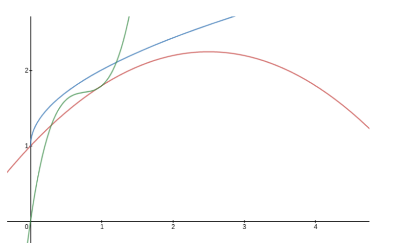
\includegraphics[width=8cm, height=5cm]{polyreg.png}
    \end{figure}

    \textbf{Red:} Quadratic

    \textbf {Blue:} Square root funtion $ \theta_0+\theta_1x+\theta_2\sqrt{x} $

    \textbf {Green:} Cubic function

\section{Normal equation}
  Normal Equation is a method to solve for $\theta_T$ analytically, by creating a $m\times(n+1)$ matrix $X$ and another $m\times1$ matrix $Y$.\footnote[2]{Every element of first column of matrix $X$ is 1 and other are the feature's coefficient}

  Mathematically $\theta$ is given as:
  \begin{equation} \label {eq: theta}
    \theta = (X^TX)^{-1}X^ty
  \end{equation}

  \begin{tabular}{ |c|c|}
    \hline
    \textbf{Gradient Descent} & \textbf{Normal Equation} \\
    \hline
    Need to choose $\alpha$ & No need to choose $\alpha$ \\
    Needs many iteration & Don't need to iterate \\
    Works well with large n & Slow for large n \\
    \hline
  \end{tabular}

  \vspace{5mm}

  \subsubsection{Reasons for non-invertiblity of $X^T X$}
    \begin{itemize}
      \item Redundant features (linear dependence) \footnote[3]{Eg. Using both $m^2 \  \& \  (feet)^2$ features}
      \item Too many features (m $<=$ n) 
    \end{itemize}


\chapter{Logistic Regression}
\section{Classification and Representation}

  \subsection{Classification}
    The classification problem is just like the regression problem, except that the values we now want to predict take on only a small number of discrete values. For now, we'll discuss a binary classification problem.

  \subsection{Hypothesis Representation}
    We may use our old regression algorithm by classifying data on the basis of a threshold. But it will have very poor performance.\\ 
    \\We will introduce "Sigmoid Function", also called the "Logistic Function":
    \begin{equation}
      h_\theta(x) = g(\theta^{T}x)
    \end{equation}
    \begin{equation}
      z = \theta^{T}x
    \end{equation}
    \begin{equation}\label{eq:sigmoid}
      g(z) = \frac{1}{1+e^{-z}}
    \end{equation}
    This is how the Sigmoid Function looks like:
    \begin{figure}[h]
      \centering
      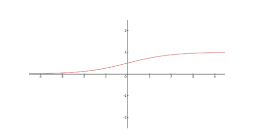
\includegraphics[scale = 0.6]{sigmoid.png}
      \caption{Sigmoid Funtion \ref{eq:sigmoid}}
    \end{figure}

  \subsection{Decesion Boundary}
    The decision boundary is the line that separates the area where y=0 and where y=1.\\
    It is similar to the decision boundary for linear regression, the only difference is the distribution of values (linear and sigmoid)

\section{Logistic Regression Model}

  \subsection{Cost Function}
    Cost funtion for logistic regression looks like:

    \begin{equation}
      J(\theta) = \frac{1}{m}\sum_{i=1}^{m}Cost(h_\theta(x^{(i)}), y^{(i)})
    \end{equation}
    \\ \\
    $ Cost(h_\theta(x),y) = -\log{(h_\theta{(x)})} $ \hfill if $y = 1$
    \\ \\
    $Cost(h_\theta(x),y) = -\log{(1-h_\theta{(x)})}$  \hfill if $y = 0$

    \begin{figure}[h]
      \centering
      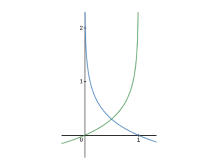
\includegraphics[scale = 0.6]{costlog.png}
      \caption{Cost Funtion}
    \end{figure}

    \subsubsection{Siplified Cost Funtion}
    This cost funtion can be compressed into a single funtion:
    \begin{equation}
      Cost(h_\theta(x),y) = -y\log{(h_\theta{(x)})} -(1-y)\log{(1-h_\theta{(x)})}
    \end{equation}
    A vectorised implementation is: \\ \\
    $h = g(X\theta)$\\
    $J(\theta) = \frac{1}{m}.(-y^T\log{h}-(1-y)^T\log{1-h})$
    \\ \\
    Vectorised implementation for Gradient Descent: \\ \\
    $\theta := \theta - \frac{\alpha}{m}X^T(g(X\theta)-y)$

\section{Multiclass Classification}
  \subsection{One-vs-all}
    This approach is when data has more than two categories.We divide our problem into n\footnote[1]{n = no of categories in dataset} binary classification problems, in each one, we predict the probability considering one of the category to be $+$ve and all other to be $-$ve. Repeating this for all other categories will finally give us all the decesion boundaries.
    \begin{figure}[h]
      \centering
      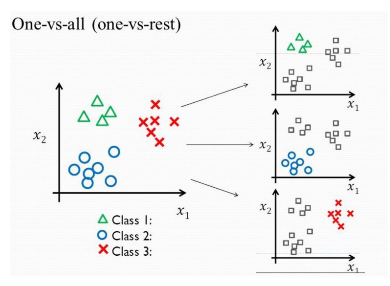
\includegraphics[scale = 0.5]{oneall.png}
      \caption{One vs all classifiaction method}
    \end{figure}   

\section{The Problem of Overfitting}
  Consider the problem of predicting y from x $\in$ R. The leftmost figure below shows the result of fitting a $y = \theta_0+\theta_1x$ to a dataset. We see that the data doesn’t really lie on straight line, and so the fit is not very good.\\ 
  \begin{figure}[h]
    \centering
    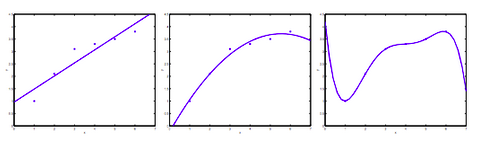
\includegraphics[scale=0.5]{overfitting.png}
  \end{figure}
  \\
  Instead, if we had added an extra feature $x^2$ , and fit $ t = \theta_0 + \theta_1x + \theta_2x^2$ , then we obtain a slightly better fit to the data (See middle figure). Naively, it might seem that the more features we add, the better. However, there is also a danger in adding too many features: The rightmost figure is the result of fitting a $5^{th}$ order polynomial $y = \sum_{j=0} ^5 \theta_j x^j$. We see that even though the fitted curve passes through the data perfectly, we would not expect this to be a very good predictor of, say, housing prices (y) for different living areas (x). Without formally defining what these terms mean, we’ll say the figure on the left shows an instance of \textbf{underfitting}—in which the data clearly shows structure not captured by the model—and the figure on the right is an example of \textbf{overfitting}.

    \subsubsection{How to address this issue?}
      \begin{enumerate}
        \item Reduce the number of features:
        \begin{itemize}
          \item Manually select which features to keep.
          \item Use a model selection algorithm.\footnote[2]{we'll cover it later}
        \end{itemize}
        \item Regularisation:
        \begin{itemize}
          \item Keep all the features, but reduce the magnitude of parameters $\theta_j$.
          \item Regularization works well when we have a lot of slightly useful features.
        \end{itemize}
      \end{enumerate}

  \subsection{Regularized Cost Function}
    To solve this problem of overfitting, we can eleminate the influence of $\theta_3x^3$ and $\theta_4x^4$. Without actually getting rid of these features or changing the form of our hypothesis, we can instead modify our cost function:
    \begin{equation}
      J_\theta = min\ of\ \left[ \frac{1}{2m} \sum_{i=1}^{m}(h_\theta(x^{(i)}) - y^{(i)})^2 + \lambda\sum_{j=1}^2\theta_j^2 \right]
    \end{equation}
    These extra terms will inflate the cost of extra parameters. \\ \\
    The $\lambda$ is called the \textbf{regularisation parameter}/ It determines how much the costs of out theta parameters are inflated.

  \subsection{Regularized Linear Regression}
    \begin{figure}[h]
      \centering
      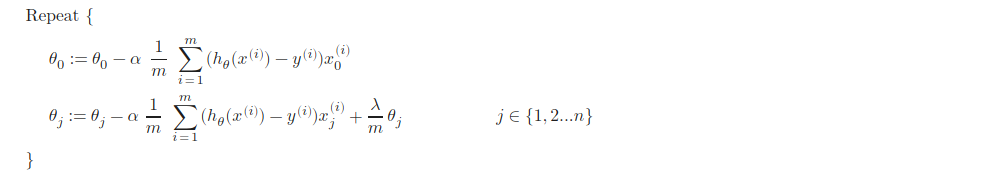
\includegraphics[scale=1]{gradregularize.png}
    \end{figure}


    The term $\frac{\lambda}{m}\theta_{j}$ performs our regularization. With some manipulation, our update rule can also be represented as \\

    $ \theta_j := \theta_j(1 - \alpha\frac{\lambda}{m}) - \alpha\frac{1}{m}\sum_{i=1}^m(h_\theta(x^{(i)}) - y^{(i)})x_j^{(i)} $\\

    The first term in the above equation, $\alpha\frac{\lambda}{m}$ will always be less than 1. Intuitively you can see it as reducing the value of $j\theta_j$ by some amount on every update.

    \subsubsection{Normal Eequation}
      This will be the non-iterative approach for regularisation.\\\\
      To add in regularization, we'll just add another term:
      \begin{equation}
        \theta = X^T X + \lambda . L^{-1} X^T y
      \end{equation}
      where, L is $(n+1)\times(n+1)$ matrix with 0 at the top lest, 1`s down the diagonal and all other element '0'.
    % \\ \\
    % \lstinputlisting[language=Octave, caption=Octave Implementation for Logistic Regression Algorithms]{logisticRegression.m}


\chapter{Decision Tree}
\documentclass[12pt, A4]{report}
\usepackage[utf8]{inputenc}

\usepackage{graphicx}
\graphicspath{{./images/}}

\usepackage{listings}
\usepackage{xcolor}

\definecolor{codegreen}{rgb}{0,0.6,0}
\definecolor{codegray}{rgb}{0.5,0.5,0.5}
\definecolor{codepurple}{rgb}{0.58,0,0.82}
\definecolor{backcolour}{rgb}{0.95,0.95,0.92}

\lstdefinestyle{mystyle}{
    backgroundcolor=\color{backcolour},   
    commentstyle=\color{codegreen},
    keywordstyle=\color{magenta},
    numberstyle=\tiny\color{codegray},
    stringstyle=\color{codepurple},
    basicstyle=\ttfamily\footnotesize,
    breakatwhitespace=false,         
    breaklines=true,                 
    captionpos=b,                    
    keepspaces=true,                 
    numbers=left,                    
    numbersep=5pt,                  
    showspaces=false,                
    showstringspaces=false,
    showtabs=false,                  
    tabsize=2
}

\lstset{style=mystyle}

\usepackage{hyperref}
\hypersetup{
    colorlinks=true,
    linkcolor=blue,
    filecolor=magenta,      
    urlcolor=cyan,
}

\urlstyle{same}


\title{\textbf{Decision Tree}\\ \large{Supervised ML Algorithm}}
\author{Sahasra Ranjan}
\date{April 2020}

\begin{document}

\begin{titlepage}
\maketitle
\end{titlepage}

A decision tree is a map of the possible outcomes of a series of a related choices. It allows to weigh possible actions against one another based of various factors.\par
It uses a tree-like model of decision. It typically starts with a single node, which branches into possible outcomes. Each of those outcomes leads to additional nodes, which branch off into other possiblities. 

\begin{figure}[h]
	\centering
	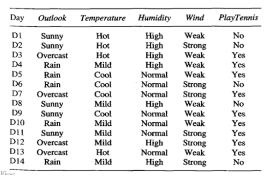
\includegraphics[width=6cm, height=4cm]{dtdata1.png}
	\caption{Dataset for possiblity of a tennis match}
	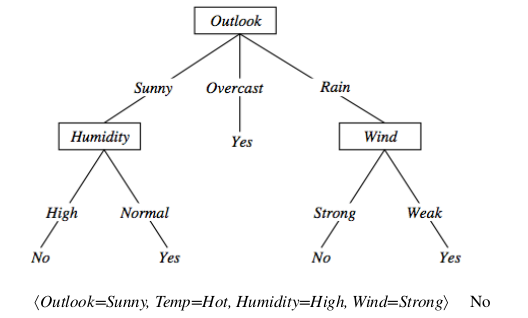
\includegraphics[width=8cm, height=5cm]{dtdata2.png}
	\caption{Decision Tree for the same}
\end{figure}

\subsection*{Advantages and Disadvantages of Decision Trees}
	\textbf{Advantages:}
	\begin{itemize}
		\item Performs classification without requiring much computation.
		\item Provides clear indication of important fields for prediction of classification.
	\end{itemize}
	\vspace{15mm}
	\textbf{Disadvantages:}
	\begin{itemize}
		\item Less appropriate for predicting continious attributes.
		\item Computationally expensive to train
	\end{itemize}

\vspace{5mm}
\subsection*{Creating a Decision Tree}
	For every node, we have to create subtrees with all the possiblities. and then further repeat for other features.\par
	For eg., In the tennis match problem, for the first node  let's check outlook, since having three possiblity (viz. Sunny, Overcast, Rainy), we created three subtrees and then further we keep asking for other features like Humidity \& wind to get the final tree.  

\vspace{5mm}
\subsection*{Greedy Approach for creating decision tree}
	Greedy approach is implemented by making an optimal local choice at each node. By making these local optimal choices, we reach the approximate optimal solution globaly.

	The algorithm can be summarized as: 
	\begin{enumerate}
		\item At each stage (node), pick out the best feature as the test conditiion.
		\item Now split the node into possibel outcomes (internal nodes)
		\item Repeat the above steps till all the test conditions have been exhausted into leaf nodes.
	\end{enumerate}

\vspace{5mm}
\subsection*{Continuous Features}
	There might be some feature which are not categorical, for these we need to create possibilities on the basis of aprropriate ranges. One such tree is shown below:
	\begin{figure}[h]
		\centering
		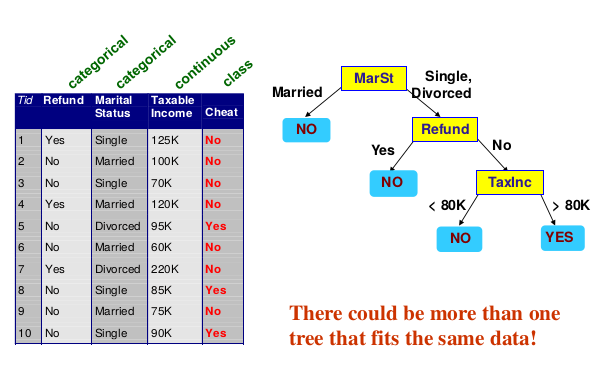
\includegraphics[width=12cm, height=6cm]{continuousDT.png}
		\caption{Decision tree with continuous feature}
	\end{figure}


\subsection*{Entropy}
	In the most layman terms, Entropy is nothing but the \textbf{The measure of disorder}.
	Why is it important to study entropy for machine learning? \\
	\\ Entropy is a measure of disorder or uncertainity and the goal of machine learning models and Data Scientists in general is to reduce uncertainity.\\
	\\ The Mathematical formula for entropy is - 
	\begin{equation}\label {eq:entropy}
		E(S) = \sum_{i=1}^c - p_i log_2 p_i\
	\end{equation}
	Where $p_i$ is the frequentist probability of an element/class $i$ in out data.\\
	\\ Let's say we have only two classes, a positive and a negative class. Out of 100 data, suppose that 70 belongs to $-$ve class and 30 to $+$ve. Then, P$+$ will be 0.3 and P$-$ will be 0.7.
	\vspace{4mm}
	Entropy $E$ will be given by:
	\begin{equation}
		E = -\frac{3}{10} \times log_2{\frac{3}{10}}-\frac{7}{10} \times log_2{\frac{7}{10}} \approx \textbf{0.88}
	\end{equation}
	\begin{figure}[h]
		\centering
		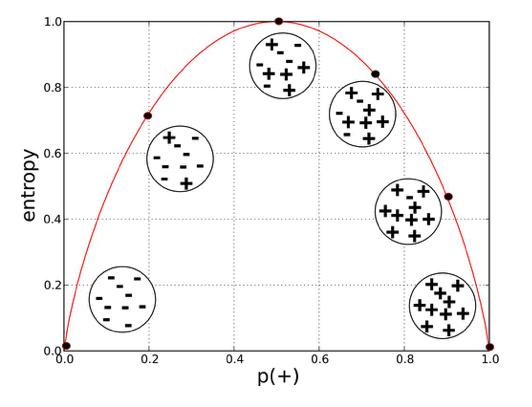
\includegraphics[width=8cm, height=6cm]{entropyDT.png}
		\caption{Entropy distribution frequentist probability}
	\end{figure}

\subsection*{Information Gain}
	Information gain is basically how much Entropy is removed after training a decision tree.\\
	\textbf{Higher information gain = more entropy removed.}\\
	In technical terms, Information Gain from X on Y is defined as:
	\begin{equation}\label{eq:inforamtion gain}
		IG(Y,X) = E(Y) - E(Y|X)
	\end{equation}
	Basics of inforation gain is well explained here: \href{https://victorzhou.com/blog/information-gain/}{A Simple Explanation of Information Gain and Entropy}

\subsection*{Example: Decision Tree}
	Consider an example where we are building a decision tree to predict whether a loan given to a person would result in a write-off or not. Our entire population consists of 30 instances. 16 belong to the write-off class and the other 14 belong to the non-write-off class. We have two features, namely “Balance” that can take on two values: “$<$ 50K” or “$>$ 50K” and “Residence” that can take on three values: “OWN”, “RENT” or “OTHER”. I’m going to show you how a decision tree algorithm would decide what attribute to split on first and what feature provides more information, or reduces more uncertainty about our target variable out of the two using the concepts of Entropy and Information Gain.
	\begin{figure}[h]
		\centering
		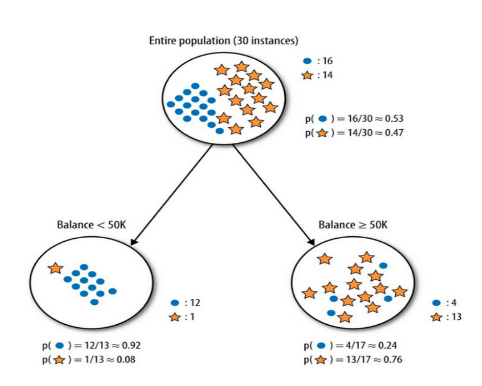
\includegraphics[width=10cm, height=7.5cm]{tree1.png}
		\caption{Feature 1: Balance}
	\end{figure}
	The dots are the data points with class right-off and the stars are the non-write-offs. Splitting the parent node on attribute balance gives us 2 child nodes. The left node gets 13 of the total observations with 12/13 ( 0.92 probability) observations from the write-off class and only 1/13( 0.08 probability) observations from the non-write of class. The right node gets 17 of the total observation with 13/17( 0.76 probability) observations from the non-write-off class and 4/17 ( 0.24 probability) from the write-off class.
	\\ \\Let’s calculate\footnote[1]{See this for calculations and further refrences: \href{https://towardsdatascience.com/entropy-how-decision-trees-make-decisions-2946b9c18c8}{Entropy: How Decision Trees Make Decisions}} the entropy for the parent node and see how much uncertainty the tree can reduce by splitting on Balance.	
	Splitting on feature ,“Balance” leads to an information gain of 0.37 on our target variable. Let’s do the same thing for feature, “Residence” to see how it compares.\\ 
	\begin{figure}[h]
		\centering
		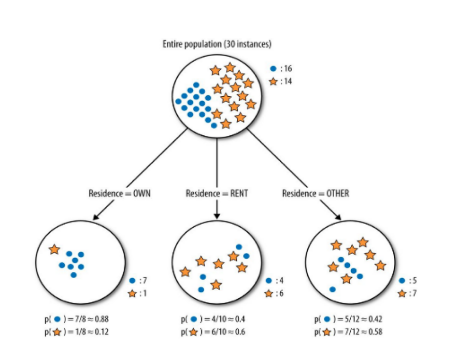
\includegraphics[width=10cm, height=7.5cm]{tree2.png}
		\caption{Feature 2: Residence}
	\end{figure}
	\\
	Splitting the tree on Residence gives us 3 child nodes. The left child node gets 8 of the total observations with 7/8 (0.88 probability) observations from the write-off class and only 1/8 (0.12 probability) observations from the non-write-off class. The middle child nodes gets 10 of the total observations with 4/10 (0.4 probability) observations of the write-off class and 6/10( 0.6 probability) observations from the non-write-off class. The right child node gets 12 of the total observations with 5/12 ( 0.42 probability) observations from the write-off class and 7/12 ( 0.58 ) observations from the non-write-off class. We already know the entropy for the parent node. We simply need to calculate the entropy after the split to compute the information gain from “Residence”

	The information gain from feature, Balance is almost 3 times more than the information gain from Residence! If you go back and take a look at the graphs you can see that the child nodes from splitting on Balance do seem purer than those of Residence. However the left most node for residence is also very pure but this is where the weighted averages come in play. Even though that node is very pure, it has the least amount of the total observations and a result contributes a small portion of it’s purity when we calculate the total entropy from splitting on Residence. This is important because we’re looking for overall informative power of a feature and we don’t want our results to be skewed by a rare value in a feature.
	\\ \\
	By itself the feature, Balance provides more information about our target variable than Residence. It reduces more disorder in our target variable. A decision tree algorithm would use this result to make the first split on our data using Balance. From here on, the decision tree algorithm would use this process at every split to decide what feature it is going to split on next. In a real world scenario , with more than two features the first split is made on the most informative feature and then at every split the information gain for each additional feature needs to be recomputed because it would not be the same as the information gain from each feature by itself. The entropy and information gain would have to be calculated after one or more splits have already been made which would change the results. A decision tree would repeat this process as it grows deeper and deeper till either it reaches a pre-defined depth or no additional split can result in a higher information gain beyond a certain threshold which can also usually be specified as a hyper-parameter!
	\\ \\
	There you have it! You now know what entropy and information gain are and how they are computed. You understand how a decision tree either by itself or in a tree based ensemble decides on the best order of features to split on and decides when to stop when it trains itself on given data. If you every have to explain the intricacies of how decision trees work to someone, hopefully you won’t do too bad.\\

\subsection*{Implementation}
\lstinputlisting[language=Octave, caption=Python Implementation for Decision Tree]{dtScratch.py}

\end{document}

\chapter{Naive Bayes}
\section*{Naive Bayes}

Naive Bayes methods are a set of supervised learning algorithms based on applying Bayes' theorem with the "naive" assumption of conditional independence between every pair of features given the value of the class variable.\\ \\
What actually Bayes' theorem is?
\begin{equation}\label {eq:bayes}
    P(A|B) = \frac{P(B|A)P(A)}{P(B)}
\end{equation}
$P(A|B)$ is the probability of \textbf{A} happening, given that \textbf{B} has occured.\\ \\ Why "Naive"? Because the presence of one particular feature does not affect the other.
\\ \\ 
Without going to deep, let's see an example:

\subsection*{The Golf Match Problem}
    Consider the problem of playing golf, dataset for the same:
    \begin{figure}[h]
        \centering
        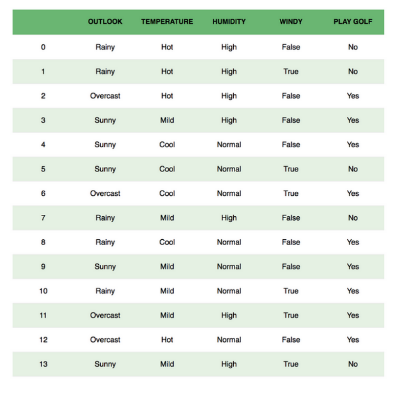
\includegraphics[scale=0.7]{golf.png}
        \caption{Dataset for possiblity of a golf match}
    \end{figure}

    Bayes theorem for this example can be rewritten as:
    \begin{equation}
        P(y|X) = \frac{P(X|y)P(y)}{P(X)}
    \end{equation}

    The variable \textbf{y} is the class variable (play golf), which represents if it is suitable to play golf or not given the conditions. Variable \textbf{X} is a matrix representing the parameters/features.
    \\ \\
    $\textbf{X} = (x_1, x_2, x_3, ... , x_n)$ \hfill    \small{$x_1, x_2, ... x_n$ represent the features}\footnote[1]{temperature, humidity and windy (here)}.
    \\ \\

    \begin{equation}
        P(y|x_1, ..., x_n) = \frac{P(x_1|y)P(x_2|y)...P(x_n|y)P(y)}{P(x_1)P(x_2)...P(x_n)}
    \end{equation}
    These values can be obtained by looking at the dataset and substituting them into the equation will give us the result.
    \\ \\
    In our case, the the class variable(\textbf{y}) has only two outcomes, yes or no. Therefore, we need to find class \textbf{y} with maximum probability. 
    \begin{equation}
        y = argmax_yP(y)\prod_{i=1}^{n}P(x_i|y)
    \end{equation}

\subsection*{Types of Naive Bayes classifier:}
    \subsubsection*{Miltinomial Naive Bayes:}
        This is mostly used for the document classification problem, i.e whether a document belongs to the category of sports, politics, technology etc. The features/predictors used by the classifier are the frequency of the words present in the document.

    \subsubsection*{Bernoulli Naive Bayes}
        This is similar to the multinomial Naive Bayes but the predictors are boolean variables. The parameters that we use to predict the class variable take up only values yes or no, for example, if a word occurs in the text or not.

    \subsubsection*{Gaussian Naive Bayes}
        When the predictors take up a continuous value and are not discrete, we assume that these values are sampled from a gaussian distribution.

        \begin{figure}[h]
            \centering
            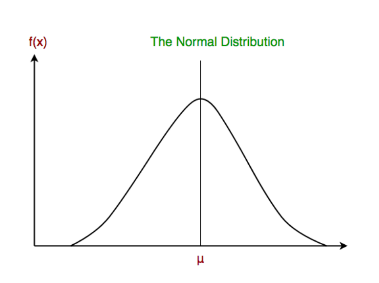
\includegraphics[scale=0.6]{gaussiannaive.png}
            \caption{Gaussian Distribution(Normal Distribution)}
        \end{figure}

        The formula for conditional probability changes to:

        \begin{equation}
            P(x_i|y) = \frac{1}{\sqrt{2\pi\sigma_y^2}}e^{-\frac{(x_i-\mu_y)^2}{2\sigma_y^2}}
        \end{equation}

\subsection*{Laplace Smoothing}
    It is problematic when a frequency-based probability is zero because it will wipe out all the information in the other probabilities.\\ \\
    A solution would be \textbf{Laplace smoothing}, which is a technique for smoothing categorical data. A small-sample correction, or \textbf{pseudo-count}, will be incorporated in every probability estimate. Consequently, no probability will be zero. this is a way of regularizing Naive Bayes, and when the pseudo-count is zero, it is called Laplace smoothing. While in the general case it is often called \textbf{Lidstone smoothing.}

    \begin{equation}
        P_{i,\ \alpha-smoothed} = \frac{x_i+\alpha}{N+\alpha d}
    \end{equation}
    where, $\alpha > 0$ the "pseudocount" is a smoothing parameter. And, $1/d$ is the \href{https://en.wikipedia.org/wiki/Discrete_uniform_distribution}{Uniform Probability}.

    \subsubsection*{Note}
    In practice, we use logs to represent probabilities:
    \begin{equation}
        \log{(P(x_1|y)P(x_2|y)...P(x_n|y))} = \log{P(x_1|y)} + \log{P(x_2|y)} +...+ \log{P(x_n|y)}
    \end{equation}


\subsection*{Applications}
    Naive Bayes algorithms are mostly used in sentiment analysis, spam filtering, recommendation systems etc. They are fast and easy to implement but their biggest disadvantage is that the requirement of predictors to be independent. In most of the real-life cases, the predictors are dependent, this hinders the performance of the classifier.

\subsection*{Worked-out Implementation\footnote[2]{ \textbf{Output:}\\
23 columns, after dropping NA, 22\\
Test 1\\
5671 correct of 5687\\
Accuracy: 0.997186565851943\\
Test 2\\
2433 correct of 2437\\
Accuracy: 0.9983586376692655\\ 
\\This implementation of Naive Bayes Algorithm has an accuracy of approximately 99.8\% which is good in the first go.}}
\lstinputlisting[language=Python, caption=Python Implementation for Naive Bayes]{naiveBayes-implementation.py}


\chapter{k-Nearest Neighbours}
\input{sections/KNN}

\chapter{Neural Networks}
  At a very simple level, neurons are basically computational units that take inputs (\textbf{dendrites}) as electrical inputs (called "spikes") that are channeled to outputs (\textbf{axons}). In our model, our dendrites are like the input features $x_1...x_n$, and the output is the result of our hypothesis function. In this model our $x_0$ input node is sometimes called the "bias unit." It is always equal to 1.

  \begin{figure}[h]
    \centering
    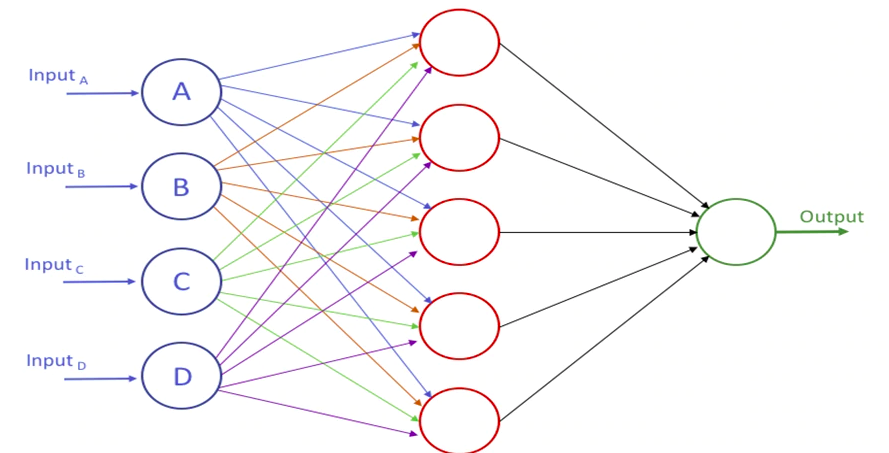
\includegraphics[scale=0.3]{neuralnetwork.png}
  \end{figure}

  Our input nodes (layer 1), also known as the "input layer", go into another node (layer 2), which finally outputs the hypothesis function, known as the "output layer". We can have intermediate layers of nodes between the input and output layers called the "hidden layers."
  \\\\
  These "hidden layer" nodes are called as "activation units". The values for each activation nodes are represented as: \\
  \begin{figure}[h]
    \centering
    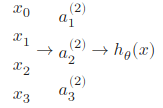
\includegraphics[scale=0.6]{hiddenlayer.png}
  \end{figure}

  \begin{equation}
    a_1^{(2)} = g(\theta_{10}^{(1)}x_0 + \theta_{11}^{(1)}x_1 + \theta_{12}^{(1)}x_2 + \theta_{13}^{(1)}x_3)
  \end{equation}
  \begin{equation}
    a_2^{(2)} = g(\theta_{20}^{(1)}x_0 + \theta_{21}^{(1)}x_1 + \theta_{22}^{(1)}x_2 + \theta_{23}^{(1)}x_3)
  \end{equation}
  \begin{equation}
    a_3^{(2)} = g(\theta_{30}^{(1)}x_0 + \theta_{31}^{(1)}x_1 + \theta_{32}^{(1)}x_2 + \theta_{33}^{(1)}x_3)
  \end{equation}
  \begin{equation}
    h_\theta(x) = a_1^{(3)]} = a_1^{(2)} = g(\theta_{10}^{(2)}x_0 + \theta_{11}^{(2)}x_1 + \theta_{12}^{(2)}x_2 + \theta_{13}^{(2)}x_3)5
  \end{equation}
  \\From these equations, we can conclude that we will get a matrix for each layer to calculate the weight for the second layer.

  \section{Intutions}
    \subsection{OR Function}
      \begin{figure}[h]
        \centering
        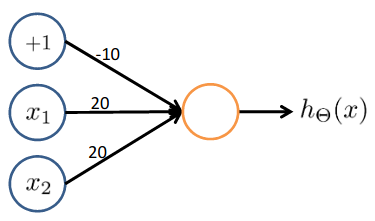
\includegraphics[scale=0.5]{ornet.png}
        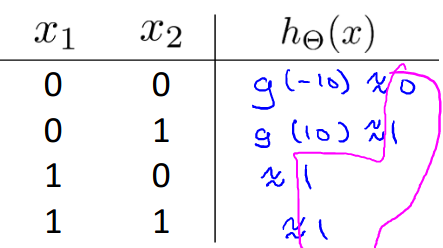
\includegraphics[scale=0.4]{ortable.png}
      \end{figure}

    \subsection{Important Note}
      \begin{figure}[h]
        \centering
        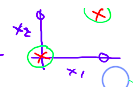
\includegraphics[scale=1]{important-net.png}
      \end{figure}

      For any prediction which involves a straight line as decision boundary, we can represent it with a neural network without any hidden layer but otherwise, we'll have to include few hidden layers. An important point to note is that we can represent almost any distribution with a certain arrangement of Neural Network.

  \section{Multiclass Classification}
    To classify data into multiple classes, we'll have to define out set of resulting classes as y:
    \begin{figure}[h]
      \centering
      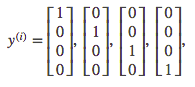
\includegraphics[scale=0.6]{resultnet.png}
    \end{figure}

  \section{Cost Function}
    Let's first define a few variables that we'll need to use:
    
    \begin{itemize}
      \item L = total number of layers in the network
      \item numbers of units (non counting bias unit) in layer 1
      \item K = numbet of output unit/classes
    \end{itemize}

    The cost function for neural networks will be slightly more complicated as it involves a few other factors of 'K' and 'L' defined earlier.

    \begin{equation}
      J(\theta) = -\frac{1}{m}\sum_{i=1}^{m}\sum_{k=1}^{K}y_k^{(i)}\log((h_\theta(x^{(i)}))_k) + (1-y_k^{(i)})\log(1-(h_\theta(x^{(i)}))_k) + \frac{\lambda}{2m}\sum_{l=1}^{L-1}\sum_{i=1}^{s_l}\sum_{j=1}^{s_{l+1}} (\theta_{j,i}^{(L)})^2
    \end{equation}

    \textbf{Note:}
    \begin{itemize}
      \item the double sum simply adds up the logistic regression costs calculated for each cell in the output layer.
      \item the triple sum simply adds up the squares of all the individual $\theta$s in the entire network.
      \item the I in the triple sum does not refer to training example i.
    \end{itemize}

  \section{Backpropagation Algorithm}
    Given training set ${(x^(1),y^(1))...(x^(m),y^(m))}$
    \begin{itemize}
      \item Set $\Delta^{(l)}_{i,j} := 0$ for all (l,i,j), (hence you end up having a matrix full of zeros)
    \end{itemize}

    For training example t=1 to m:
    \begin{enumerate}
      \item Set $a^{(1)} := x^{(t)}$
      \item Perform forward propagation to compute $a^{(l)}$ for l = 2,3,...,L

      \textbf{Gradient Computation}

      \item Using $y^{(t)}$, compute $\delta^{(L)} = a^{(L)} - y^{(L)}$
      \item Compute $\delta^{(l)}$
      \item $\Delta^{(L)} := \Delta^{(L)} + \delta^{(l+1)}(a^{(l)})^T$

      \begin{figure}[h]
        
\includegraphics[scale=0.65]{bpupdate.png}
      \end{figure}
    \end{enumerate}

  \section{Gradient Checking}
    Gradient checking will assure that our backpropagation works as intended. We can approximate the derivative of our cost function with:

    \begin{figure}[h]
      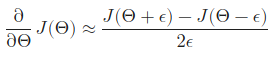
\includegraphics[scale=0.65]{gc.png}
    \end{figure}

    And for multiple features,

    \begin{figure}[h]
      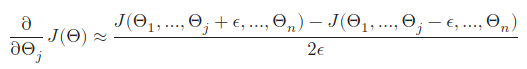
\includegraphics[scale=0.65]{gcmult.png}
    \end{figure}

  \section{Putting it Together}
    First, pick a network architecture; choose the layout of your neural network, including how many hidden units in each layer and how many layers in total you want to have.

    \begin{itemize}
      \item Number of input units = dimension of features $x^{(i)}$
      \item Number of output units = number of classes
      \item Number of hidden units per layer = usually more the better (must balance with the cost of computation as it increases with more hidden units)
      \item Defaults: 1 hidden layer. If you have more than 1 hidden layer, then it is recommended that you have the same number of units in every hidden layer.
    \end{itemize}

    \subsubsection{Training a Neural Network}
      \begin{enumerate}
        \item Randomly initialize the weights\footnote[3]{A good choice for $e_init = \frac{\sqrt{6}}{\sqrt{L_in + L_out}}$}
        \item Implement forward propagation to get $h_\theta(x(i))$ for any $x^{(i)}$
        \item Implement the cost function
        \item Implement backpropagation to compute partial derivatives
        \item Use gradient checking to confirm that your backpropagation works. Then disable gradient checking.
        \item Use gradient descent or a built-in optimization function to minimize the cost function with the weights in theta.
      \end{enumerate}

  % \lstinputlisting[language=octave, caption=Octave implementation for section of Neural Networks]{3.NeuralNetwork.m}

\chapter{Improving Neural Networks}
What to try next for improving our neural networks?
\begin{itemize}
  \item Getting more training examples
  \item Trying smaller sets of features
  \item Trying additional features
  \item Trying polynomial features
  \item Increasing or decreasing $\lambda$
\end{itemize}

\section{Evaulating a Hypothesis}
A hypothesis may have a low error for training examples but still be inaccurate (because of overfitting). Thus, to evaulate a hypothesis, given a dataset of training examples, we can split up the data into two sets: a training set and a test set. Typically, the training set consists of $70\%$ of your data and the test set is the remaining $30\% $.

\begin{figure}[h]
  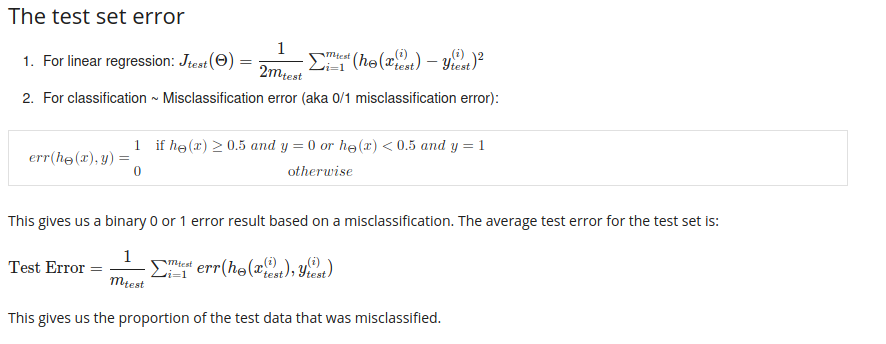
\includegraphics[scale=0.5]{testerror.png}
\end{figure}

\subsection{Model Selection}
  Just because a learning algorithm fits a training set well, that does not mean it is a good hypothesis. It could over fit and as a result your predictions on the test set would be poor.
  \\\\
  Given many models with different polynomial degrees, we can use a systematic approach to identify the 'best' function. In order to choose the model of your hypothesis, you can test each degree of polynomial and look at the error result.
  \\\\
  We usually break down out dataset into three sets:
  \begin{itemize}
    \item Training set: $60\%$
    \item Cross validation set: $20\%$
    \item Test set: $20\%$
  \end{itemize}


  Now to improve our training:
  \begin{enumerate}
    \item Optimize the parameters in $\theta$ using training set.
    \item Find the polynomial degree $d$ with the least error usign the cross validation set.
    \item Estimate the generalization error using the test set with $J_{test}(\Theta^{(d)})$ (d = $\theta$ from polynomial with lower error)
  \end{enumerate}

\section{Bias vs. Variance}
  \textbf{High bias (underfitting)}: both $J_train(\theta)$ and $J_{CV}(\theta)$ will be high and also similar.
  \\\\
  \textbf{High variance (overfitting)}: $J_train(\theta)$ will be low but $J_{CV}(\theta)$.\\

  \begin{figure}[h]
    \centering
    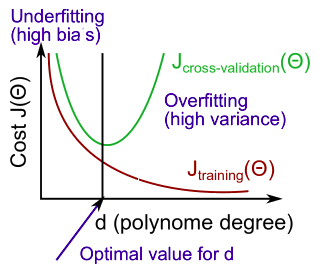
\includegraphics[scale=0.5]{biasVariance.png}
  \end{figure}

  \subsection{Regularization}

    \begin{figure}[h]
      \centering
      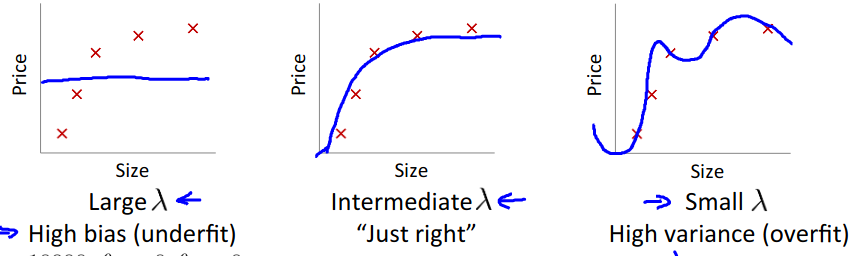
\includegraphics[scale=0.5]{lambda.png}
      \caption{Fitting of data with $\lambda$}
    \end{figure}

    In the figure above, we see that as $\lambda$ increases, our fit becomes more rigid. On the other hand, as $\lambda$ approaches 0, we tend to over overfit the data. So how do we choose our parameter $\lambda$ to get it 'just right' ?

    \begin{enumerate}
      \item Create a list of lambdas.
      \item Iterate through the $\lambda s$ and for each, go throught all the models to learn some $\theta$
      \item Compute the cross validation error.
      \item Select the best combo of $\theta \& \lambda$.
    \end{enumerate}    

  \subsection{Learning Curves}
    \begin{figure}[h]
      \centering
      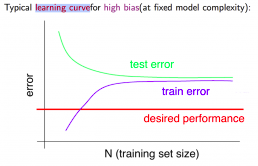
\includegraphics[scale=0.7]{learnbias.png}
      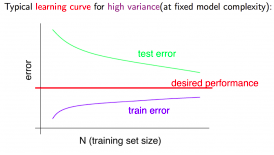
\includegraphics[scale=0.75]{learnvariance.png}
    \end{figure}    
  


\chapter{Support Vector Machines}
  The objective of the support vector machine algorithm is to find a hyperplane in N-dimensional space(N — the number of features) that distinctly classify the data points.

  To separate the two classes of data points, there are many possible hyperplanes that could be chosen. Our objective is to find a plane that has the maximum margin, i.e the maximum distance between data points of both classes. Maximizing the margin distance provides some reinforcement so that future data points can be classified with more confidence.

  \section{Hyperplanes and Support Vectors}

      Hyperplanes are decision boundaries that help classify the data points. Data points falling on either side of the hyperplane can be attributed to different classes. Also, the dimension of the hyperplane depends upon the number of features. If the number of input features is 2, then the hyperplane is just a line. If the number of input features is 3, then the hyperplane becomes a two-dimensional plane. It becomes difficult to imagine when the number of features exceeds 3.

      \begin{figure}[h]
          \centering
        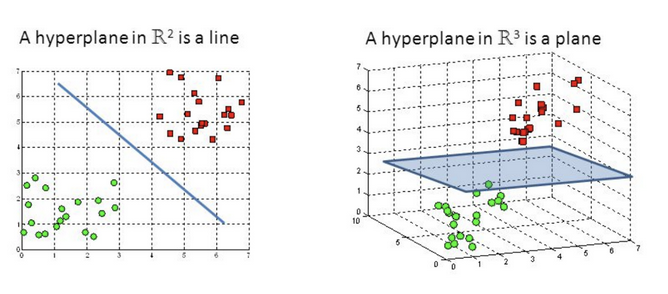
\includegraphics[scale = 0.4]{svm1.png}
    \end{figure}

      Support vectors are data points that are closer to the hyperplane and influence the position and orientation of the hyperplane. Using these support vectors, we maximize the margin of the classifier. Deleting the support vectors will change the position of the hyperplane. These are the points that help us build our SVM.

  \section{Large Margin Intuition}
      In logistic regression, we take the output of the linear function and squash the value within the range of [0,1] using the sigmoid function. If the squashed value is greater than a threshold value(0.5) we assign it a label 1, else we assign it a label 0. In SVM, we take the output of the linear function and if that output is greater than 1, we identify it with one class and if the output is -1, we identify is with another class. Since the threshold values are changed to 1 and -1 in SVM, we obtain this reinforcement range of values([-1,1]) which acts as margin.


      \begin{figure}[h]
          \centering
        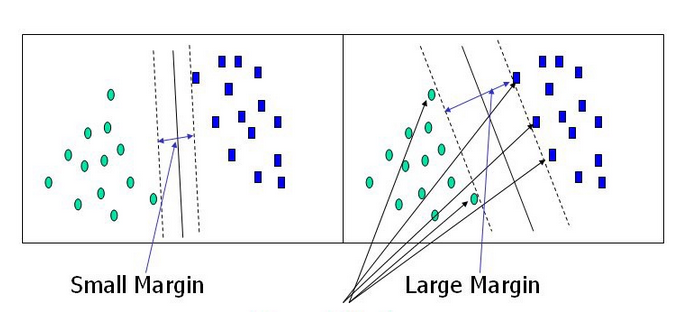
\includegraphics[scale = 0.4]{svm2.png}
        \caption{Support Vectors}
    \end{figure}
      

  % \lstinputlisting[language=octave, caption=Octave implementation for Support Vector Machines]{6 svm.m}


\chapter{Unsupervised Learning}
Unsupervised learning is a type of machine learning that looks for previously undetected patterns in a data set with no pre-existing labels and with a minimum of human supervision. In contrast to supervised learning that usually makes use of human-labeled data, unsupervised learning, also known as self-organization allows for modeling of probability densities over inputs. It forms one of the three main categories of machine learning, along with supervised and reinforcement learning. Semi-supervised learning, a related variant, makes use of supervised and unsupervised techniques.

\section{K-Means Clustering Algorithm}
	Kmeans algorithm is an iterative algorithm that tries to partition the dataset into K pre-defined distinct non-overlapping subgroups (clusters) where each data point belongs to only one group. It tries to make the intra-cluster data points as similar as possible while also keeping the clusters as different (far) as possible. It assigns data points to a cluster such that the sum of the squared distance between the data points and the cluster’s centroid (arithmetic mean of all the data points that belong to that cluster) is at the minimum. The less variation we have within clusters, the more homogeneous (similar) the data points are within the same cluster.\\\\

	The way kmeans algorithm works is as follows:
	\begin{enumerate}
		\item Specify number of clusters K.
		\item Initialize centroids by first shuffling the dataset and then randomly selecting K data points for the centroids without replacement.
		\item Keep iterating until there is no change to the centroids. i.e assignment of data points to clusters isn’t changing: 
		\begin{itemize}
			\item Compute the sum of the squared distance between data points and all centroids.
			\item Assign each data point to the closest cluster (centroid).
			\item Compute the centroids for the clusters by taking the average of the all data points that belong to each cluster.
		\end{itemize}
	\end{enumerate}

	\subsection{\textbf{The Elbow Method}: Choosing the number of clusters}
		For the k-means clustering method, the most common approach for choosing the number of clusters is the so-called \textbf{elbow method}. It involves running the algorithm multiple times over a loop, with an increasing number of cluster choice and then plotting a clustering score as a function of the number of clusters.\\

		What is the score or metric which is being plotted for the elbow method? Why is it called the ‘elbow’ method?\\

		A typical plot looks like following,

		\begin{figure}[h]
			\centering
			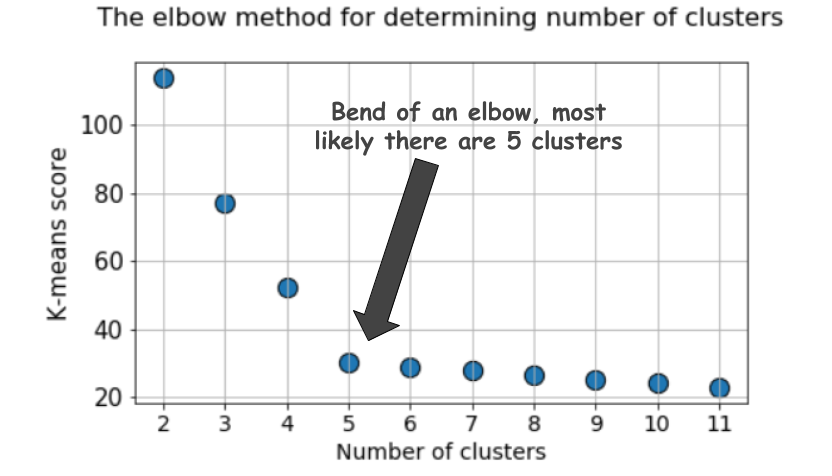
\includegraphics[scale=0.35]{elbow.png}
			\caption{Elbow Method: Score plot}
		\end{figure}

		The score is, in general, a measure of the input data on the k-means objective function i.e. \textbf{some form of intra-cluster distance relative to inner-cluster distance}.
  \section{Anamoly Detection}
  Anomaly detection is the process of identifying unexpected items or events in data sets, which differ from the norm. And anomaly detection is often applied to unlabeled data which is known as unsupervised anomaly detection. Anomaly detection has two basic assumptions:

\begin{itemize}
    \item Anomalies only occur very rarely in the data.
    \item Their features differ from the normal instances significantly.
\end{itemize}
    
% \lstinputlisting[language=Octave, caption=Octave implementation for Anamoly Detection]{8 Anamoly Detection.m}

\chapter{Convolutional neural network}
A Convolutional Neural Network (ConvNet/CNN) is a Deep Learning algorithm that can take in an input image, assign importance (learnable weights and biases) to various aspects/objects in the image, and be able to differentiate one from the other. The pre-processing required in a ConvNet is much lower as compared to other classification algorithms. While in primitive methods filters are hand-engineered, with enough training, ConvNets have the ability to learn these filters/characteristics.
\\ \\
The architecture of a ConvNet is analogous to that of the connectivity pattern of Neurons in the Human Brain and was inspired by the organization of the Visual Cortex. Individual neurons respond to stimuli only in a restricted region of the visual field known as the Receptive Field. A collection of such fields overlap to cover the entire visual area.
\\ \\
The Convolutional Neural Networks enable machines to view the world as humans do, perceive it in a similar manner and even use the knowledge for a multitude of tasks such as Image $\&$ Video recognition, Image Analysis $\&$ Classification, Media Recreation, Recommendation Systems, Natural Language Processing, etc. 

\begin{figure}[h]
    \centering
    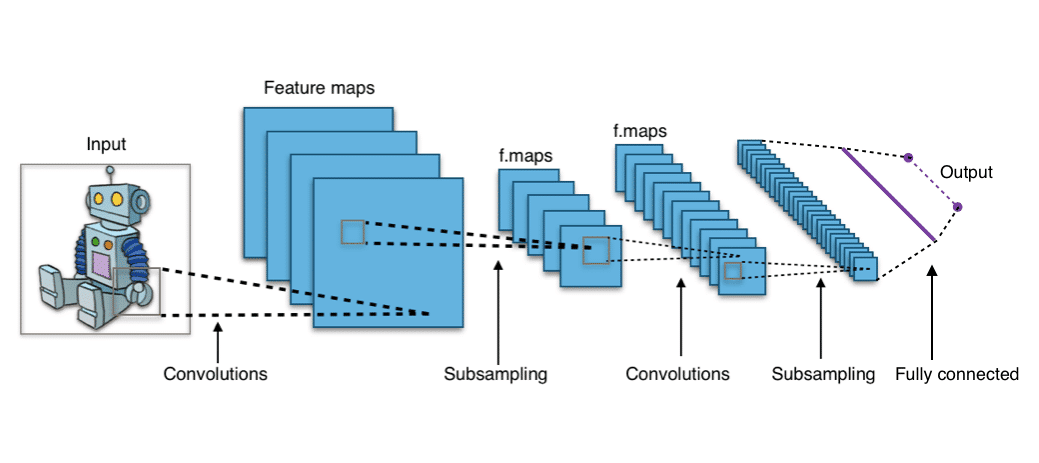
\includegraphics[scale=0.4]{CNN4.png}
    \caption{Convolutional Neural Network}
\end{figure}

\section{CNNs vs Feed-forward Neural Nets!}
    An image is nothing but a matrix of pixel values, right? So why not just flatten the image (e.g. 3x3 image matrix into a 9x1 vector) and feed it to a Multi-Level Perceptron for classification purposes?
\\ \\
    In cases of extremely basic binary images, the method might show an average precision score while performing prediction of classes but would have little to no accuracy when it comes to complex images having pixel dependencies throughout.
\\ \\
    A ConvNet is able to successfully capture the Spatial and Temporal dependencies in an image through the application of relevant filters. The architecture performs a better fitting to the image dataset due to the reduction in the number of parameters involved and the reusability of weights. In other words, the network can be trained to understand the sophistication of the image better.

\section{Convolution Layer — The Kernel}
    Each convolutional layer contains a series of filters known as convolutional kernels. The filter is a matrix of integers that are used on a subset of the input pixel values, the same size as the kernel. Each pixel is multiplied by the corresponding value in the kernel, then the result is summed up for a single value for simplicity representing a grid cell, like a pixel, in the output channel/feature map. These are linear transformations, each convolution is a type of affine function.

    \begin{figure}[h]
        \centering
        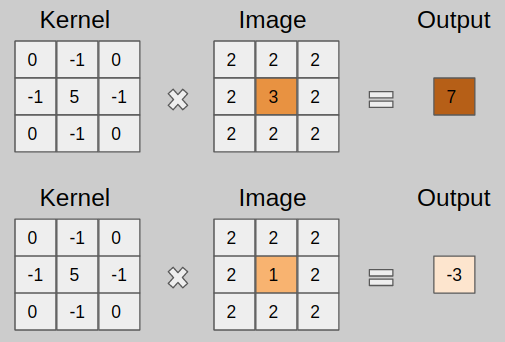
\includegraphics[scale=0.4]{CNN3.png}
        \caption{Average and Max pooling layer}
    \end{figure}

    In computer vision, the input is often a 3 channel RGB image. For simplicity, if we take a greyscale image that has one channel (a two-dimensional matrix) and a 3x3 convolutional kernel (a two-dimensional matrix). The kernel strides over the input matrix of numbers moving horizontally column by column, sliding/scanning over the first rows in the matrix containing the images pixel values. Then the kernel strides down vertically to subsequent rows. Note, the filter may stride over one or several pixels at a time, this is detailed further below. In other non-vision applications, a one-dimensional convolution may slide vertically over an input matrix.

\section{Pooling Layer}
    Similar to the Convolutional Layer, the Pooling layer is responsible for reducing the spatial size of the Convolved Feature. This is to decrease the computational power required to process the data through dimensionality reduction. Furthermore, it is useful for extracting dominant features that are rotational and positional invariant, thus maintaining the process of effectively training of the model.
\\ \\
    There are two types of Pooling: Max Pooling and Average Pooling. Max Pooling returns the maximum value from the portion of the image covered by the Kernel. On the other hand, Average Pooling returns the average of all the values from the portion of the image covered by the Kernel.

    \begin{figure}[h]
        \centering
        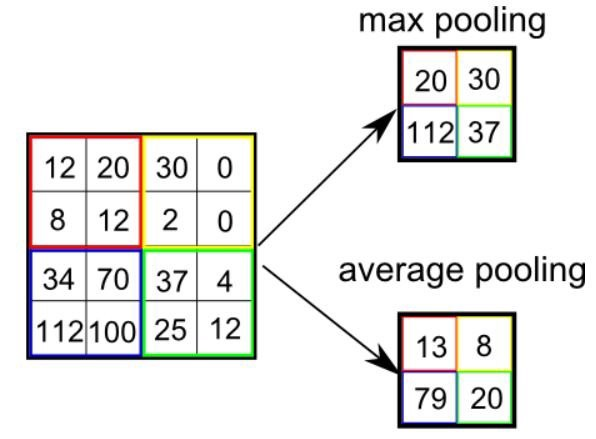
\includegraphics[scale=0.4]{CNN1.jpeg}
        \caption{Average and Max pooling layer}
    \end{figure}

    Max Pooling also performs as a Noise Suppressant. It discards the noisy activations altogether and also performs de-noising along with dimensionality reduction. On the other hand, Average Pooling simply performs dimensionality reduction as a noise suppressing mechanism. Hence, we can say that Max Pooling performs a lot better than Average Pooling.
\\ \\
    The Convolutional Layer and the Pooling Layer, together form the i-th layer of a Convolutional Neural Network. Depending on the complexities in the images, the number of such layers may be increased for capturing low-levels details even further, but at the cost of more computational power.
\\ \\
    After going through the above process, we have successfully enabled the model to understand the features. Moving on, we are going to flatten the final output and feed it to a regular Neural Network for classification purposes.


\chapter{PyTorch Implementations}

  \section{Perceptrons}
  Perceptron is a single layer neural network and a multi-layer perceptron is called Neural Networks. Here, we'll try to implement a basic perceptron based model to classify between dataset with two labels.

     \begin{tcolorbox}[breakable, size=fbox, boxrule=1pt, pad at break*=1mm,colback=cellbackground, colframe=cellborder]
\prompt{In}{incolor}{1}{\boxspacing}
\begin{Verbatim}[commandchars=\\\{\}]
\PY{k+kn}{import} \PY{n+nn}{torch}
\PY{k+kn}{import} \PY{n+nn}{numpy} \PY{k}{as} \PY{n+nn}{np}
\PY{k+kn}{import} \PY{n+nn}{matplotlib}\PY{n+nn}{.}\PY{n+nn}{pyplot} \PY{k}{as} \PY{n+nn}{plt}
\PY{k+kn}{import} \PY{n+nn}{torch}\PY{n+nn}{.}\PY{n+nn}{nn} \PY{k}{as} \PY{n+nn}{nn}
\PY{k+kn}{from} \PY{n+nn}{sklearn} \PY{k+kn}{import} \PY{n}{datasets}
\end{Verbatim}
\end{tcolorbox}

    \begin{tcolorbox}[breakable, size=fbox, boxrule=1pt, pad at break*=1mm,colback=cellbackground, colframe=cellborder]
\prompt{In}{incolor}{2}{\boxspacing}
\begin{Verbatim}[commandchars=\\\{\}]
  \PY{n}{n\PYZus{}pts} \PY{o}{=} \PY{l+m+mi}{100}
  \PY{n}{centers} \PY{o}{=} \PY{p}{[}\PY{p}{[}\PY{o}{\PYZhy{}}\PY{l+m+mf}{0.5}\PY{p}{,} \PY{l+m+mf}{0.5}\PY{p}{]}\PY{p}{,} \PY{p}{[}\PY{l+m+mf}{0.5}\PY{p}{,} \PY{o}{\PYZhy{}}\PY{l+m+mf}{0.5}\PY{p}{]}\PY{p}{]}
  \PY{n}{X}\PY{p}{,} \PY{n}{y} \PY{o}{=} \PY{n}{datasets}\PY{o}{.}\PY{n}{make\PYZus{}blobs}\PY{p}{(}\PY{n}{n\PYZus{}samples}\PY{o}{=}\PY{n}{n\PYZus{}pts}\PY{p}{,} \PY{n}{random\PYZus{}state}\PY{o}{=}\PY{l+m+mi}{123}\PY{p}{,} \PY{n}{centers}\PY{o}{=}\PY{n}{centers}\PY{p}{,} \PY{n}{cluster\PYZus{}std}\PY{o}{=}\PY{l+m+mf}{0.4}\PY{p}{)}
  
  \PY{n}{x\PYZus{}data} \PY{o}{=} \PY{n}{torch}\PY{o}{.}\PY{n}{Tensor}\PY{p}{(}\PY{n}{X}\PY{p}{)}
  \PY{n}{y\PYZus{}data} \PY{o}{=} \PY{n}{torch}\PY{o}{.}\PY{n}{Tensor}\PY{p}{(}\PY{n}{y}\PY{o}{.}\PY{n}{reshape}\PY{p}{(}\PY{l+m+mi}{100}\PY{p}{,} \PY{l+m+mi}{1}\PY{p}{)}\PY{p}{)}
  \PY{n+nb}{print}\PY{p}{(}\PY{n}{y}\PY{o}{.}\PY{n}{shape}\PY{p}{)}
\end{Verbatim}
\end{tcolorbox}

    \begin{Verbatim}[commandchars=\\\{\}]
(100,)
    \end{Verbatim}

    \begin{tcolorbox}[breakable, size=fbox, boxrule=1pt, pad at break*=1mm,colback=cellbackground, colframe=cellborder]
\prompt{In}{incolor}{3}{\boxspacing}
\begin{Verbatim}[commandchars=\\\{\}]
\PY{k}{def} \PY{n+nf}{scatter\PYZus{}plot}\PY{p}{(}\PY{p}{)}\PY{p}{:}
    \PY{n}{plt}\PY{o}{.}\PY{n}{scatter}\PY{p}{(}\PY{n}{X}\PY{p}{[}\PY{n}{y}\PY{o}{==}\PY{l+m+mi}{0}\PY{p}{,} \PY{l+m+mi}{0}\PY{p}{]}\PY{p}{,} \PY{n}{X}\PY{p}{[}\PY{n}{y}\PY{o}{==}\PY{l+m+mi}{0}\PY{p}{,} \PY{l+m+mi}{1}\PY{p}{]}\PY{p}{)} \PY{c+c1}{\PYZsh{} Blue}
    \PY{n}{plt}\PY{o}{.}\PY{n}{scatter}\PY{p}{(}\PY{n}{X}\PY{p}{[}\PY{n}{y}\PY{o}{==}\PY{l+m+mi}{1}\PY{p}{,} \PY{l+m+mi}{0}\PY{p}{]}\PY{p}{,} \PY{n}{X}\PY{p}{[}\PY{n}{y}\PY{o}{==}\PY{l+m+mi}{1}\PY{p}{,} \PY{l+m+mi}{1}\PY{p}{]}\PY{p}{)} \PY{c+c1}{\PYZsh{} Orange}
\end{Verbatim}
\end{tcolorbox}

    \begin{tcolorbox}[breakable, size=fbox, boxrule=1pt, pad at break*=1mm,colback=cellbackground, colframe=cellborder]
\prompt{In}{incolor}{4}{\boxspacing}
\begin{Verbatim}[commandchars=\\\{\}]
\PY{n}{scatter\PYZus{}plot}\PY{p}{(}\PY{p}{)}
\end{Verbatim}
\end{tcolorbox}

    \begin{center}
    \adjustimage{max size={0.9\linewidth}{0.9\paperheight}}{Perceptron_files/Perceptron_3_0.png}
    \end{center}
    { \hspace*{\fill} \\}
    
    \begin{tcolorbox}[breakable, size=fbox, boxrule=1pt, pad at break*=1mm,colback=cellbackground, colframe=cellborder]
\prompt{In}{incolor}{5}{\boxspacing}
\begin{Verbatim}[commandchars=\\\{\}]
\PY{k}{class} \PY{n+nc}{Model}\PY{p}{(}\PY{n}{nn}\PY{o}{.}\PY{n}{Module}\PY{p}{)}\PY{p}{:}
    \PY{k}{def} \PY{n+nf+fm}{\PYZus{}\PYZus{}init\PYZus{}\PYZus{}}\PY{p}{(}\PY{n+nb+bp}{self}\PY{p}{,} \PY{n}{input\PYZus{}size}\PY{p}{,} \PY{n}{output\PYZus{}size}\PY{p}{)}\PY{p}{:}
      \PY{n+nb}{super}\PY{p}{(}\PY{p}{)}\PY{o}{.}\PY{n+nf+fm}{\PYZus{}\PYZus{}init\PYZus{}\PYZus{}}\PY{p}{(}\PY{p}{)} 
      \PY{n+nb+bp}{self}\PY{o}{.}\PY{n}{linear} \PY{o}{=} \PY{n}{nn}\PY{o}{.}\PY{n}{Linear}\PY{p}{(}\PY{n}{input\PYZus{}size}\PY{p}{,} \PY{n}{output\PYZus{}size}\PY{p}{)}
    \PY{k}{def} \PY{n+nf}{forward}\PY{p}{(}\PY{n+nb+bp}{self}\PY{p}{,} \PY{n}{x}\PY{p}{)}\PY{p}{:}
      \PY{n}{pred} \PY{o}{=} \PY{n}{torch}\PY{o}{.}\PY{n}{sigmoid}\PY{p}{(}\PY{n+nb+bp}{self}\PY{o}{.}\PY{n}{linear}\PY{p}{(}\PY{n}{x}\PY{p}{)}\PY{p}{)}
      \PY{k}{return} \PY{n}{pred}
    \PY{k}{def} \PY{n+nf}{predict}\PY{p}{(}\PY{n+nb+bp}{self}\PY{p}{,} \PY{n}{x}\PY{p}{)}\PY{p}{:}
      \PY{n}{pred} \PY{o}{=} \PY{n+nb+bp}{self}\PY{o}{.}\PY{n}{forward}\PY{p}{(}\PY{n}{x}\PY{p}{)}
      \PY{k}{if} \PY{n}{pred} \PY{o}{\PYZgt{}}\PY{o}{=} \PY{l+m+mf}{0.5}\PY{p}{:}
        \PY{k}{return} \PY{l+m+mi}{1}
      \PY{k}{else}\PY{p}{:}
        \PY{k}{return} \PY{l+m+mi}{0}
\end{Verbatim}
\end{tcolorbox}

    \begin{tcolorbox}[breakable, size=fbox, boxrule=1pt, pad at break*=1mm,colback=cellbackground, colframe=cellborder]
\prompt{In}{incolor}{6}{\boxspacing}
\begin{Verbatim}[commandchars=\\\{\}]
\PY{n}{torch}\PY{o}{.}\PY{n}{manual\PYZus{}seed}\PY{p}{(}\PY{l+m+mi}{2}\PY{p}{)}
\PY{n}{model} \PY{o}{=} \PY{n}{Model}\PY{p}{(}\PY{l+m+mi}{2}\PY{p}{,} \PY{l+m+mi}{1}\PY{p}{)}
\PY{n+nb}{print}\PY{p}{(}\PY{n+nb}{list}\PY{p}{(}\PY{n}{model}\PY{o}{.}\PY{n}{parameters}\PY{p}{(}\PY{p}{)}\PY{p}{)}\PY{p}{)}
\end{Verbatim}
\end{tcolorbox}

    \begin{Verbatim}[commandchars=\\\{\}]
[Parameter containing:
tensor([[ 0.1622, -0.1683]], requires\_grad=True), Parameter containing:
tensor([0.1939], requires\_grad=True)]
    \end{Verbatim}

    \begin{tcolorbox}[breakable, size=fbox, boxrule=1pt, pad at break*=1mm,colback=cellbackground, colframe=cellborder]
\prompt{In}{incolor}{7}{\boxspacing}
\begin{Verbatim}[commandchars=\\\{\}]
\PY{p}{[}\PY{n}{w}\PY{p}{,} \PY{n}{b}\PY{p}{]} \PY{o}{=} \PY{n}{model}\PY{o}{.}\PY{n}{parameters}\PY{p}{(}\PY{p}{)}
\PY{n}{w1}\PY{p}{,} \PY{n}{w2} \PY{o}{=} \PY{n}{w}\PY{o}{.}\PY{n}{view}\PY{p}{(}\PY{l+m+mi}{2}\PY{p}{)}
\PY{k}{def} \PY{n+nf}{get\PYZus{}params}\PY{p}{(}\PY{p}{)}\PY{p}{:}
  \PY{k}{return} \PY{p}{(}\PY{n}{w1}\PY{o}{.}\PY{n}{item}\PY{p}{(}\PY{p}{)}\PY{p}{,} \PY{n}{w2}\PY{o}{.}\PY{n}{item}\PY{p}{(}\PY{p}{)}\PY{p}{,} \PY{n}{b}\PY{p}{[}\PY{l+m+mi}{0}\PY{p}{]}\PY{o}{.}\PY{n}{item}\PY{p}{(}\PY{p}{)}\PY{p}{)}
\end{Verbatim}
\end{tcolorbox}

    \begin{tcolorbox}[breakable, size=fbox, boxrule=1pt, pad at break*=1mm,colback=cellbackground, colframe=cellborder]
\prompt{In}{incolor}{8}{\boxspacing}
\begin{Verbatim}[commandchars=\\\{\}]
\PY{k}{def} \PY{n+nf}{plot\PYZus{}fit}\PY{p}{(}\PY{n}{title}\PY{p}{)}\PY{p}{:}
    \PY{n}{plt}\PY{o}{.}\PY{n}{title} \PY{o}{=} \PY{n}{title}
    \PY{n}{w1}\PY{p}{,} \PY{n}{w2}\PY{p}{,} \PY{n}{b1} \PY{o}{=} \PY{n}{get\PYZus{}params}\PY{p}{(}\PY{p}{)}
    \PY{n}{x1} \PY{o}{=} \PY{n}{np}\PY{o}{.}\PY{n}{array}\PY{p}{(}\PY{p}{[}\PY{o}{\PYZhy{}}\PY{l+m+mf}{2.0}\PY{p}{,} \PY{l+m+mf}{2.0}\PY{p}{]}\PY{p}{)}
    \PY{n}{x2} \PY{o}{=} \PY{o}{\PYZhy{}}\PY{l+m+mi}{1}\PY{o}{*}\PY{p}{(}\PY{n}{w1}\PY{o}{*}\PY{n}{x1} \PY{o}{+} \PY{n}{b1}\PY{p}{)}\PY{o}{/}\PY{n}{w2}
    \PY{n}{scatter\PYZus{}plot}\PY{p}{(}\PY{p}{)}
    \PY{n}{plt}\PY{o}{.}\PY{n}{plot}\PY{p}{(}\PY{n}{x1}\PY{p}{,} \PY{n}{x2}\PY{p}{,} \PY{l+s+s1}{\PYZsq{}}\PY{l+s+s1}{r}\PY{l+s+s1}{\PYZsq{}}\PY{p}{)}
    \PY{n}{plt}\PY{o}{.}\PY{n}{show}\PY{p}{(}\PY{p}{)}
\end{Verbatim}
\end{tcolorbox}

    \begin{tcolorbox}[breakable, size=fbox, boxrule=1pt, pad at break*=1mm,colback=cellbackground, colframe=cellborder]
\prompt{In}{incolor}{9}{\boxspacing}
\begin{Verbatim}[commandchars=\\\{\}]
\PY{n}{plot\PYZus{}fit}\PY{p}{(}\PY{l+s+s1}{\PYZsq{}}\PY{l+s+s1}{Initial Model}\PY{l+s+s1}{\PYZsq{}}\PY{p}{)}
\end{Verbatim}
\end{tcolorbox}

    \begin{center}
    \adjustimage{max size={0.9\linewidth}{0.9\paperheight}}{Perceptron_files/Perceptron_8_0.png}
    \end{center}
    { \hspace*{\fill} \\}
    
    \begin{tcolorbox}[breakable, size=fbox, boxrule=1pt, pad at break*=1mm,colback=cellbackground, colframe=cellborder]
\prompt{In}{incolor}{10}{\boxspacing}
\begin{Verbatim}[commandchars=\\\{\}]
\PY{n}{criterion} \PY{o}{=} \PY{n}{nn}\PY{o}{.}\PY{n}{BCELoss}\PY{p}{(}\PY{p}{)}
\PY{n}{optimizer} \PY{o}{=} \PY{n}{torch}\PY{o}{.}\PY{n}{optim}\PY{o}{.}\PY{n}{SGD}\PY{p}{(}\PY{n}{model}\PY{o}{.}\PY{n}{parameters}\PY{p}{(}\PY{p}{)}\PY{p}{,} \PY{n}{lr}\PY{o}{=}\PY{l+m+mf}{0.01}\PY{p}{)}
\end{Verbatim}
\end{tcolorbox}

    \begin{tcolorbox}[breakable, size=fbox, boxrule=1pt, pad at break*=1mm,colback=cellbackground, colframe=cellborder]
\prompt{In}{incolor}{11}{\boxspacing}
\begin{Verbatim}[commandchars=\\\{\}]
\PY{n}{epochs} \PY{o}{=} \PY{l+m+mi}{1000}
\PY{n}{losses} \PY{o}{=} \PY{p}{[}\PY{p}{]}

\PY{k}{for} \PY{n}{i} \PY{o+ow}{in} \PY{n+nb}{range}\PY{p}{(}\PY{n}{epochs}\PY{p}{)}\PY{p}{:}
  \PY{n}{y\PYZus{}pred} \PY{o}{=} \PY{n}{model}\PY{o}{.}\PY{n}{forward}\PY{p}{(}\PY{n}{x\PYZus{}data}\PY{p}{)}
  \PY{n}{loss} \PY{o}{=} \PY{n}{criterion}\PY{p}{(}\PY{n}{y\PYZus{}pred}\PY{p}{,} \PY{n}{y\PYZus{}data}\PY{p}{)}
  \PY{n+nb}{print}\PY{p}{(}\PY{l+s+s2}{\PYZdq{}}\PY{l+s+s2}{epoch:}\PY{l+s+s2}{\PYZdq{}}\PY{p}{,} \PY{n}{i}\PY{p}{,} \PY{l+s+s2}{\PYZdq{}}\PY{l+s+s2}{loss:}\PY{l+s+s2}{\PYZdq{}}\PY{p}{,} \PY{n}{loss}\PY{o}{.}\PY{n}{item}\PY{p}{(}\PY{p}{)}\PY{p}{)}
  \PY{n}{losses}\PY{o}{.}\PY{n}{append}\PY{p}{(}\PY{n}{loss}\PY{o}{.}\PY{n}{item}\PY{p}{(}\PY{p}{)}\PY{p}{)}
  \PY{n}{optimizer}\PY{o}{.}\PY{n}{zero\PYZus{}grad}\PY{p}{(}\PY{p}{)}
  \PY{n}{loss}\PY{o}{.}\PY{n}{backward}\PY{p}{(}\PY{p}{)}
  \PY{n}{optimizer}\PY{o}{.}\PY{n}{step}\PY{p}{(}\PY{p}{)}
\end{Verbatim}
\end{tcolorbox}

    \begin{Verbatim}[commandchars=\\\{\}]
epoch: 0 loss: 0.6185115575790405
epoch: 1 loss: 0.617464005947113
epoch: 2 loss: 0.6164200305938721
.
.
.
epoch: 999 loss: 0.2561521828174591
    \end{Verbatim}

    \begin{tcolorbox}[breakable, size=fbox, boxrule=1pt, pad at break*=1mm,colback=cellbackground, colframe=cellborder]
\prompt{In}{incolor}{12}{\boxspacing}
\begin{Verbatim}[commandchars=\\\{\}]
\PY{n}{plt}\PY{o}{.}\PY{n}{plot}\PY{p}{(}\PY{n+nb}{range}\PY{p}{(}\PY{n}{epochs}\PY{p}{)}\PY{p}{,} \PY{n}{losses}\PY{p}{)}
\PY{n}{plt}\PY{o}{.}\PY{n}{ylabel}\PY{p}{(}\PY{l+s+s1}{\PYZsq{}}\PY{l+s+s1}{Loss}\PY{l+s+s1}{\PYZsq{}}\PY{p}{)}
\PY{n}{plt}\PY{o}{.}\PY{n}{xlabel}\PY{p}{(}\PY{l+s+s1}{\PYZsq{}}\PY{l+s+s1}{epochs}\PY{l+s+s1}{\PYZsq{}}\PY{p}{)}
\PY{n}{plt}\PY{o}{.}\PY{n}{grid}\PY{p}{(}\PY{p}{)}
\end{Verbatim}
\end{tcolorbox}

    \begin{center}
    \adjustimage{max size={0.9\linewidth}{0.9\paperheight}}{Perceptron_files/Perceptron_11_0.png}
    \end{center}
    { \hspace*{\fill} \\}
    
    \begin{tcolorbox}[breakable, size=fbox, boxrule=1pt, pad at break*=1mm,colback=cellbackground, colframe=cellborder]
\prompt{In}{incolor}{13}{\boxspacing}
\begin{Verbatim}[commandchars=\\\{\}]
\PY{n}{plot\PYZus{}fit}\PY{p}{(}\PY{l+s+s2}{\PYZdq{}}\PY{l+s+s2}{Trained Model}\PY{l+s+s2}{\PYZdq{}}\PY{p}{)}
\end{Verbatim}
\end{tcolorbox}

    \begin{center}
    \adjustimage{max size={0.9\linewidth}{0.9\paperheight}}{Perceptron_files/Perceptron_12_0.png}
    \end{center}
    { \hspace*{\fill} \\}
    
    \begin{tcolorbox}[breakable, size=fbox, boxrule=1pt, pad at break*=1mm,colback=cellbackground, colframe=cellborder]
\prompt{In}{incolor}{17}{\boxspacing}
\begin{Verbatim}[commandchars=\\\{\}]
\PY{n}{point1} \PY{o}{=} \PY{n}{torch}\PY{o}{.}\PY{n}{tensor}\PY{p}{(}\PY{p}{[}\PY{l+m+mf}{1.0}\PY{p}{,} \PY{o}{\PYZhy{}}\PY{l+m+mf}{1.0}\PY{p}{]}\PY{p}{)}
\PY{n}{point2} \PY{o}{=} \PY{n}{torch}\PY{o}{.}\PY{n}{tensor}\PY{p}{(}\PY{p}{[}\PY{o}{\PYZhy{}}\PY{l+m+mf}{1.0}\PY{p}{,} \PY{l+m+mf}{1.0}\PY{p}{]}\PY{p}{)}
\PY{n}{plt}\PY{o}{.}\PY{n}{plot}\PY{p}{(}\PY{n}{point1}\PY{o}{.}\PY{n}{numpy}\PY{p}{(}\PY{p}{)}\PY{p}{[}\PY{l+m+mi}{0}\PY{p}{]}\PY{p}{,} \PY{n}{point1}\PY{o}{.}\PY{n}{numpy}\PY{p}{(}\PY{p}{)}\PY{p}{[}\PY{l+m+mi}{1}\PY{p}{]}\PY{p}{,} \PY{l+s+s1}{\PYZsq{}}\PY{l+s+s1}{go}\PY{l+s+s1}{\PYZsq{}}\PY{p}{)}
\PY{n}{plt}\PY{o}{.}\PY{n}{plot}\PY{p}{(}\PY{n}{point2}\PY{o}{.}\PY{n}{numpy}\PY{p}{(}\PY{p}{)}\PY{p}{[}\PY{l+m+mi}{0}\PY{p}{]}\PY{p}{,} \PY{n}{point2}\PY{o}{.}\PY{n}{numpy}\PY{p}{(}\PY{p}{)}\PY{p}{[}\PY{l+m+mi}{1}\PY{p}{]}\PY{p}{,} \PY{l+s+s1}{\PYZsq{}}\PY{l+s+s1}{ko}\PY{l+s+s1}{\PYZsq{}}\PY{p}{)}
\PY{n}{plot\PYZus{}fit}\PY{p}{(}\PY{l+s+s2}{\PYZdq{}}\PY{l+s+s2}{Trained Model}\PY{l+s+s2}{\PYZdq{}}\PY{p}{)}

\PY{n+nb}{print}\PY{p}{(}\PY{l+s+s2}{\PYZdq{}}\PY{l+s+s2}{Red point positive probability = }\PY{l+s+si}{\PYZob{}\PYZcb{}}\PY{l+s+s2}{\PYZdq{}}\PY{o}{.}\PY{n}{format}\PY{p}{(}\PY{n}{model}\PY{o}{.}\PY{n}{forward}\PY{p}{(}\PY{n}{point1}\PY{p}{)}\PY{o}{.}\PY{n}{item}\PY{p}{(}\PY{p}{)}\PY{p}{)}\PY{p}{)} 
\PY{n+nb}{print}\PY{p}{(}\PY{l+s+s2}{\PYZdq{}}\PY{l+s+s2}{Black point positive probability = }\PY{l+s+si}{\PYZob{}\PYZcb{}}\PY{l+s+s2}{\PYZdq{}}\PY{o}{.}\PY{n}{format}\PY{p}{(}\PY{n}{model}\PY{o}{.}\PY{n}{forward}\PY{p}{(}\PY{n}{point2}\PY{p}{)}\PY{o}{.}\PY{n}{item}\PY{p}{(}\PY{p}{)}\PY{p}{)}\PY{p}{)} 
\PY{n+nb}{print}\PY{p}{(}\PY{l+s+s2}{\PYZdq{}}\PY{l+s+s2}{Red point belongs in class }\PY{l+s+si}{\PYZob{}\PYZcb{}}\PY{l+s+s2}{\PYZdq{}}\PY{o}{.}\PY{n}{format}\PY{p}{(}\PY{n}{model}\PY{o}{.}\PY{n}{predict}\PY{p}{(}\PY{n}{point1}\PY{p}{)}\PY{p}{)}\PY{p}{)} 
\PY{n+nb}{print}\PY{p}{(}\PY{l+s+s2}{\PYZdq{}}\PY{l+s+s2}{Black point belongs in class = }\PY{l+s+si}{\PYZob{}\PYZcb{}}\PY{l+s+s2}{\PYZdq{}}\PY{o}{.}\PY{n}{format}\PY{p}{(}\PY{n}{model}\PY{o}{.}\PY{n}{predict}\PY{p}{(}\PY{n}{point2}\PY{p}{)}\PY{p}{)}\PY{p}{)} 
\end{Verbatim}
\end{tcolorbox}

    \begin{center}
    \adjustimage{max size={0.9\linewidth}{0.9\paperheight}}{Perceptron_files/Perceptron_13_0.png}
    \end{center}
    { \hspace*{\fill} \\}
    
    \begin{Verbatim}[commandchars=\\\{\}]
Red point positive probability = 0.9424158334732056
Black point positive probability = 0.05055497586727142
Red point belongs in class 1
Black point belongs in class = 0
    \end{Verbatim}

  \newpage

  \section{Linear Regression}
  Linear Regression is already discussed in the report, here, we'll try to develop a model for the same. Cell $[5]$ is our model for linear regression and input size and output size are 2 and 1 respectively.
      
    \begin{tcolorbox}[breakable, size=fbox, boxrule=1pt, pad at break*=1mm,colback=cellbackground, colframe=cellborder]
\prompt{In}{incolor}{1}{\boxspacing}
\begin{Verbatim}[commandchars=\\\{\}]
\PY{k+kn}{import} \PY{n+nn}{torch}
\PY{k+kn}{import} \PY{n+nn}{torch}\PY{n+nn}{.}\PY{n+nn}{nn} \PY{k}{as} \PY{n+nn}{nn}
\PY{k+kn}{import} \PY{n+nn}{matplotlib}\PY{n+nn}{.}\PY{n+nn}{pyplot} \PY{k}{as} \PY{n+nn}{plt}
\PY{k+kn}{import} \PY{n+nn}{numpy} \PY{k}{as} \PY{n+nn}{np}
\end{Verbatim}
\end{tcolorbox}

    \begin{tcolorbox}[breakable, size=fbox, boxrule=1pt, pad at break*=1mm,colback=cellbackground, colframe=cellborder]
\prompt{In}{incolor}{2}{\boxspacing}
\begin{Verbatim}[commandchars=\\\{\}]
\PY{n}{X} \PY{o}{=} \PY{n}{torch}\PY{o}{.}\PY{n}{randn}\PY{p}{(}\PY{l+m+mi}{100}\PY{p}{,} \PY{l+m+mi}{1}\PY{p}{)}\PY{o}{*}\PY{l+m+mi}{10}
\PY{n}{y} \PY{o}{=} \PY{n}{X} \PY{o}{+} \PY{l+m+mi}{3}\PY{o}{*}\PY{n}{torch}\PY{o}{.}\PY{n}{randn}\PY{p}{(}\PY{l+m+mi}{100}\PY{p}{,} \PY{l+m+mi}{1}\PY{p}{)}
\PY{n}{plt}\PY{o}{.}\PY{n}{plot}\PY{p}{(}\PY{n}{X}\PY{o}{.}\PY{n}{numpy}\PY{p}{(}\PY{p}{)}\PY{p}{,} \PY{n}{y}\PY{o}{.}\PY{n}{numpy}\PY{p}{(}\PY{p}{)}\PY{p}{,} \PY{l+s+s1}{\PYZsq{}}\PY{l+s+s1}{o}\PY{l+s+s1}{\PYZsq{}}\PY{p}{)}
\PY{n}{plt}\PY{o}{.}\PY{n}{ylabel}\PY{p}{(}\PY{l+s+s1}{\PYZsq{}}\PY{l+s+s1}{y}\PY{l+s+s1}{\PYZsq{}}\PY{p}{)}
\PY{n}{plt}\PY{o}{.}\PY{n}{xlabel}\PY{p}{(}\PY{l+s+s1}{\PYZsq{}}\PY{l+s+s1}{x}\PY{l+s+s1}{\PYZsq{}}\PY{p}{)}
\end{Verbatim}
\end{tcolorbox}

            \begin{tcolorbox}[breakable, size=fbox, boxrule=.5pt, pad at break*=1mm, opacityfill=0]
\prompt{Out}{outcolor}{2}{\boxspacing}
\begin{Verbatim}[commandchars=\\\{\}]
Text(0.5, 0, 'x')
\end{Verbatim}
\end{tcolorbox}
        
    \begin{center}
    \adjustimage{max size={0.9\linewidth}{0.9\paperheight}}{Linear Regression_files/Linear Regression_1_1.png}
    \end{center}
    { \hspace*{\fill} \\}
    
    \begin{tcolorbox}[breakable, size=fbox, boxrule=1pt, pad at break*=1mm,colback=cellbackground, colframe=cellborder]
\prompt{In}{incolor}{3}{\boxspacing}
\begin{Verbatim}[commandchars=\\\{\}]
\PY{k}{class} \PY{n+nc}{LR}\PY{p}{(}\PY{n}{nn}\PY{o}{.}\PY{n}{Module}\PY{p}{)}\PY{p}{:}
  \PY{k}{def} \PY{n+nf+fm}{\PYZus{}\PYZus{}init\PYZus{}\PYZus{}}\PY{p}{(}\PY{n+nb+bp}{self}\PY{p}{,} \PY{n}{input\PYZus{}size}\PY{p}{,} \PY{n}{output\PYZus{}size}\PY{p}{)}\PY{p}{:}
    \PY{n+nb}{super}\PY{p}{(}\PY{p}{)}\PY{o}{.}\PY{n+nf+fm}{\PYZus{}\PYZus{}init\PYZus{}\PYZus{}}\PY{p}{(}\PY{p}{)}
    \PY{n+nb+bp}{self}\PY{o}{.}\PY{n}{linear} \PY{o}{=} \PY{n}{nn}\PY{o}{.}\PY{n}{Linear}\PY{p}{(}\PY{n}{input\PYZus{}size}\PY{p}{,} \PY{n}{output\PYZus{}size}\PY{p}{)}
  \PY{k}{def} \PY{n+nf}{forward}\PY{p}{(}\PY{n+nb+bp}{self}\PY{p}{,} \PY{n}{x}\PY{p}{)}\PY{p}{:}
    \PY{n}{pred} \PY{o}{=} \PY{n+nb+bp}{self}\PY{o}{.}\PY{n}{linear}\PY{p}{(}\PY{n}{x}\PY{p}{)}
    \PY{k}{return} \PY{n}{pred}
\end{Verbatim}
\end{tcolorbox}

    \begin{tcolorbox}[breakable, size=fbox, boxrule=1pt, pad at break*=1mm,colback=cellbackground, colframe=cellborder]
\prompt{In}{incolor}{4}{\boxspacing}
\begin{Verbatim}[commandchars=\\\{\}]
\PY{n}{torch}\PY{o}{.}\PY{n}{manual\PYZus{}seed}\PY{p}{(}\PY{l+m+mi}{1}\PY{p}{)}
\PY{n}{model} \PY{o}{=} \PY{n}{LR}\PY{p}{(}\PY{l+m+mi}{1}\PY{p}{,} \PY{l+m+mi}{1}\PY{p}{)}
\PY{n+nb}{print}\PY{p}{(}\PY{n}{model}\PY{p}{)}
\end{Verbatim}
\end{tcolorbox}

    \begin{Verbatim}[commandchars=\\\{\}]
LR(
  (linear): Linear(in\_features=1, out\_features=1, bias=True)
)
    \end{Verbatim}

    \begin{tcolorbox}[breakable, size=fbox, boxrule=1pt, pad at break*=1mm,colback=cellbackground, colframe=cellborder]
\prompt{In}{incolor}{5}{\boxspacing}
\begin{Verbatim}[commandchars=\\\{\}]
\PY{p}{[}\PY{n}{w}\PY{p}{,}\PY{n}{b}\PY{p}{]} \PY{o}{=} \PY{n}{model}\PY{o}{.}\PY{n}{parameters}\PY{p}{(}\PY{p}{)}

\PY{k}{def} \PY{n+nf}{get\PYZus{}params}\PY{p}{(}\PY{p}{)}\PY{p}{:}
    \PY{k}{return} \PY{p}{(}\PY{n}{w}\PY{p}{[}\PY{l+m+mi}{0}\PY{p}{]}\PY{p}{[}\PY{l+m+mi}{0}\PY{p}{]}\PY{o}{.}\PY{n}{item}\PY{p}{(}\PY{p}{)}\PY{p}{,} \PY{n}{b}\PY{p}{[}\PY{l+m+mi}{0}\PY{p}{]}\PY{o}{.}\PY{n}{item}\PY{p}{(}\PY{p}{)}\PY{p}{)}
\end{Verbatim}
\end{tcolorbox}

    \begin{tcolorbox}[breakable, size=fbox, boxrule=1pt, pad at break*=1mm,colback=cellbackground, colframe=cellborder]
\prompt{In}{incolor}{6}{\boxspacing}
\begin{Verbatim}[commandchars=\\\{\}]
\PY{k}{def} \PY{n+nf}{plot\PYZus{}fit}\PY{p}{(}\PY{n}{title}\PY{p}{)}\PY{p}{:}
  \PY{n}{plt}\PY{o}{.}\PY{n}{title} \PY{o}{=} \PY{n}{title}
  \PY{n}{w1}\PY{p}{,} \PY{n}{b1} \PY{o}{=} \PY{n}{get\PYZus{}params}\PY{p}{(}\PY{p}{)}
  \PY{n}{x1} \PY{o}{=} \PY{n}{np}\PY{o}{.}\PY{n}{array}\PY{p}{(}\PY{p}{[}\PY{o}{\PYZhy{}}\PY{l+m+mi}{30}\PY{p}{,} \PY{l+m+mi}{30}\PY{p}{]}\PY{p}{)}
  \PY{n}{y1} \PY{o}{=} \PY{n}{w1}\PY{o}{*}\PY{n}{x1} \PY{o}{+} \PY{n}{b1}
  \PY{n}{plt}\PY{o}{.}\PY{n}{plot}\PY{p}{(}\PY{n}{x1}\PY{p}{,} \PY{n}{y1}\PY{p}{,} \PY{l+s+s1}{\PYZsq{}}\PY{l+s+s1}{r}\PY{l+s+s1}{\PYZsq{}}\PY{p}{)}
  \PY{n}{plt}\PY{o}{.}\PY{n}{scatter}\PY{p}{(}\PY{n}{X}\PY{p}{,} \PY{n}{y}\PY{p}{)}
  \PY{n}{plt}\PY{o}{.}\PY{n}{show}\PY{p}{(}\PY{p}{)}
\end{Verbatim}
\end{tcolorbox}

    \begin{tcolorbox}[breakable, size=fbox, boxrule=1pt, pad at break*=1mm,colback=cellbackground, colframe=cellborder]
\prompt{In}{incolor}{7}{\boxspacing}
\begin{Verbatim}[commandchars=\\\{\}]
\PY{n}{plot\PYZus{}fit}\PY{p}{(}\PY{l+s+s1}{\PYZsq{}}\PY{l+s+s1}{Initial Model}\PY{l+s+s1}{\PYZsq{}}\PY{p}{)}
\end{Verbatim}
\end{tcolorbox}

    \begin{center}
    \adjustimage{max size={0.9\linewidth}{0.9\paperheight}}{Linear Regression_files/Linear Regression_6_0.png}
    \end{center}
    { \hspace*{\fill} \\}
    
    \begin{tcolorbox}[breakable, size=fbox, boxrule=1pt, pad at break*=1mm,colback=cellbackground, colframe=cellborder]
\prompt{In}{incolor}{8}{\boxspacing}
\begin{Verbatim}[commandchars=\\\{\}]
\PY{n}{criterion} \PY{o}{=} \PY{n}{nn}\PY{o}{.}\PY{n}{MSELoss}\PY{p}{(}\PY{p}{)}
\PY{n}{optimizer} \PY{o}{=} \PY{n}{torch}\PY{o}{.}\PY{n}{optim}\PY{o}{.}\PY{n}{SGD}\PY{p}{(}\PY{n}{model}\PY{o}{.}\PY{n}{parameters}\PY{p}{(}\PY{p}{)}\PY{p}{,} \PY{n}{lr} \PY{o}{=} \PY{l+m+mf}{0.01}\PY{p}{)}
\end{Verbatim}
\end{tcolorbox}

    \begin{tcolorbox}[breakable, size=fbox, boxrule=1pt, pad at break*=1mm,colback=cellbackground, colframe=cellborder]
\prompt{In}{incolor}{9}{\boxspacing}
\begin{Verbatim}[commandchars=\\\{\}]
\PY{n}{epochs} \PY{o}{=} \PY{l+m+mi}{100}
\PY{n}{losses} \PY{o}{=} \PY{p}{[}\PY{p}{]}
\PY{k}{for} \PY{n}{i} \PY{o+ow}{in} \PY{n+nb}{range}\PY{p}{(}\PY{n}{epochs}\PY{p}{)}\PY{p}{:}
  \PY{n}{y\PYZus{}pred} \PY{o}{=} \PY{n}{model}\PY{o}{.}\PY{n}{forward}\PY{p}{(}\PY{n}{X}\PY{p}{)}
  \PY{n}{loss} \PY{o}{=} \PY{n}{criterion}\PY{p}{(}\PY{n}{y\PYZus{}pred}\PY{p}{,} \PY{n}{y}\PY{p}{)}
  \PY{n+nb}{print}\PY{p}{(}\PY{l+s+s2}{\PYZdq{}}\PY{l+s+s2}{epoch:}\PY{l+s+s2}{\PYZdq{}}\PY{p}{,} \PY{n}{i}\PY{p}{,} \PY{l+s+s2}{\PYZdq{}}\PY{l+s+s2}{loss:}\PY{l+s+s2}{\PYZdq{}}\PY{p}{,} \PY{n}{loss}\PY{o}{.}\PY{n}{item}\PY{p}{(}\PY{p}{)}\PY{p}{)}
  
  \PY{n}{losses}\PY{o}{.}\PY{n}{append}\PY{p}{(}\PY{n}{loss}\PY{p}{)}
  \PY{n}{optimizer}\PY{o}{.}\PY{n}{zero\PYZus{}grad}\PY{p}{(}\PY{p}{)}
  \PY{n}{loss}\PY{o}{.}\PY{n}{backward}\PY{p}{(}\PY{p}{)}
  \PY{n}{optimizer}\PY{o}{.}\PY{n}{step}\PY{p}{(}\PY{p}{)}
\end{Verbatim}
\end{tcolorbox}

    \begin{Verbatim}[commandchars=\\\{\}]
epoch: 0 loss: 28.098552703857422
epoch: 1 loss: 23.643329620361328
epoch: 2 loss: 20.250816345214844
.
.
.
epoch: 99 loss: 9.178099632263184
    \end{Verbatim}

    \begin{tcolorbox}[breakable, size=fbox, boxrule=1pt, pad at break*=1mm,colback=cellbackground, colframe=cellborder]
\prompt{In}{incolor}{10}{\boxspacing}
\begin{Verbatim}[commandchars=\\\{\}]
\PY{n}{plt}\PY{o}{.}\PY{n}{plot}\PY{p}{(}\PY{n+nb}{range}\PY{p}{(}\PY{n}{epochs}\PY{p}{)}\PY{p}{,} \PY{n}{losses}\PY{p}{)}
\PY{n}{plt}\PY{o}{.}\PY{n}{ylabel}\PY{p}{(}\PY{l+s+s1}{\PYZsq{}}\PY{l+s+s1}{Loss}\PY{l+s+s1}{\PYZsq{}}\PY{p}{)}
\PY{n}{plt}\PY{o}{.}\PY{n}{xlabel}\PY{p}{(}\PY{l+s+s1}{\PYZsq{}}\PY{l+s+s1}{Epochs}\PY{l+s+s1}{\PYZsq{}}\PY{p}{)}
\end{Verbatim}
\end{tcolorbox}

            \begin{tcolorbox}[breakable, size=fbox, boxrule=.5pt, pad at break*=1mm, opacityfill=0]
\prompt{Out}{outcolor}{10}{\boxspacing}
\begin{Verbatim}[commandchars=\\\{\}]
Text(0.5, 0, 'Epochs')
\end{Verbatim}
\end{tcolorbox}
        
    \begin{center}
    \adjustimage{max size={0.9\linewidth}{0.9\paperheight}}{Linear Regression_files/Linear Regression_9_1.png}
    \end{center}
    { \hspace*{\fill} \\}
    
    \begin{tcolorbox}[breakable, size=fbox, boxrule=1pt, pad at break*=1mm,colback=cellbackground, colframe=cellborder]
\prompt{In}{incolor}{11}{\boxspacing}
\begin{Verbatim}[commandchars=\\\{\}]
\PY{n}{plot\PYZus{}fit}\PY{p}{(}\PY{l+s+s2}{\PYZdq{}}\PY{l+s+s2}{Trained Model}\PY{l+s+s2}{\PYZdq{}}\PY{p}{)}
\end{Verbatim}
\end{tcolorbox}

    \begin{center}
    \adjustimage{max size={0.9\linewidth}{0.9\paperheight}}{Linear Regression_files/Linear Regression_10_0.png}
    \end{center}
    { \hspace*{\fill} \\}
    

  \newpage

  \section{Titanic Survival}
      \textbf{Problem:}\\

    The sinking of the Titanic is one of the most infamous shipwrecks in history.

    On April 15, 1912, during her maiden voyage, the widely considered “unsinkable” RMS Titanic sank after colliding with an iceberg. Unfortunately, there weren’t enough lifeboats for everyone on board, resulting in the death of 1502 out of 2224 passengers and crew.

    While there was some element of luck involved in surviving, it seems some groups of people were more likely to survive than others.

    In this challenge, we ask you to build a predictive model that answers the question: “what sorts of people were more likely to survive?” using passenger data (ie name, age, gender, socio-economic class, etc).


    \begin{tcolorbox}[breakable, size=fbox, boxrule=1pt, pad at break*=1mm,colback=cellbackground, colframe=cellborder]
  \prompt{In}{incolor}{1}{\boxspacing}
  \begin{Verbatim}[commandchars=\\\{\}]
  \PY{k+kn}{import} \PY{n+nn}{numpy} \PY{k}{as} \PY{n+nn}{np}
  \PY{k+kn}{import} \PY{n+nn}{torch}
  \PY{k+kn}{import} \PY{n+nn}{torch}\PY{n+nn}{.}\PY{n+nn}{nn} \PY{k}{as} \PY{n+nn}{nn}
  \PY{k+kn}{import} \PY{n+nn}{pandas} \PY{k}{as} \PY{n+nn}{dd}
  \PY{k+kn}{import} \PY{n+nn}{matplotlib}\PY{n+nn}{.}\PY{n+nn}{pyplot} \PY{k}{as} \PY{n+nn}{plt}
  \end{Verbatim}
  \end{tcolorbox}

      \begin{tcolorbox}[breakable, size=fbox, boxrule=1pt, pad at break*=1mm,colback=cellbackground, colframe=cellborder]
  \prompt{In}{incolor}{2}{\boxspacing}
  \begin{Verbatim}[commandchars=\\\{\}]
  \PY{n}{device} \PY{o}{=} \PY{n}{torch}\PY{o}{.}\PY{n}{device}\PY{p}{(}\PY{l+s+s2}{\PYZdq{}}\PY{l+s+s2}{cuda:0}\PY{l+s+s2}{\PYZdq{}}\PY{p}{)}
  \end{Verbatim}
  \end{tcolorbox}

      \begin{tcolorbox}[breakable, size=fbox, boxrule=1pt, pad at break*=1mm,colback=cellbackground, colframe=cellborder]
  \prompt{In}{incolor}{3}{\boxspacing}
  \begin{Verbatim}[commandchars=\\\{\}]
  \PY{n}{X} \PY{o}{=} \PY{n}{dd}\PY{o}{.}\PY{n}{read\PYZus{}csv}\PY{p}{(}\PY{l+s+s1}{\PYZsq{}}\PY{l+s+s1}{train.csv}\PY{l+s+s1}{\PYZsq{}}\PY{p}{,} \PY{n}{encoding}\PY{o}{=}\PY{l+s+s2}{\PYZdq{}}\PY{l+s+s2}{UTF\PYZhy{}8}\PY{l+s+s2}{\PYZdq{}}\PY{p}{)}
  \PY{n}{X} \PY{o}{=} \PY{n}{X}\PY{o}{.}\PY{n}{drop}\PY{p}{(}\PY{p}{[}\PY{l+s+s1}{\PYZsq{}}\PY{l+s+s1}{PassengerId}\PY{l+s+s1}{\PYZsq{}}\PY{p}{,} \PY{l+s+s1}{\PYZsq{}}\PY{l+s+s1}{Survived}\PY{l+s+s1}{\PYZsq{}}\PY{p}{,} \PY{l+s+s1}{\PYZsq{}}\PY{l+s+s1}{Ticket}\PY{l+s+s1}{\PYZsq{}}\PY{p}{,} \PY{l+s+s1}{\PYZsq{}}\PY{l+s+s1}{Name}\PY{l+s+s1}{\PYZsq{}}\PY{p}{,} \PY{l+s+s1}{\PYZsq{}}\PY{l+s+s1}{Cabin}\PY{l+s+s1}{\PYZsq{}}\PY{p}{]}\PY{p}{,} \PY{n}{axis}\PY{o}{=}\PY{l+m+mi}{1}\PY{p}{)}

  \PY{n}{y} \PY{o}{=} \PY{n}{dd}\PY{o}{.}\PY{n}{read\PYZus{}csv}\PY{p}{(}\PY{l+s+s1}{\PYZsq{}}\PY{l+s+s1}{train.csv}\PY{l+s+s1}{\PYZsq{}}\PY{p}{,} \PY{n}{usecols}\PY{o}{=}\PY{p}{[}\PY{l+s+s1}{\PYZsq{}}\PY{l+s+s1}{Survived}\PY{l+s+s1}{\PYZsq{}}\PY{p}{]}\PY{p}{)}
  \end{Verbatim}
  \end{tcolorbox}

      \begin{tcolorbox}[breakable, size=fbox, boxrule=1pt, pad at break*=1mm,colback=cellbackground, colframe=cellborder]
  \prompt{In}{incolor}{4}{\boxspacing}
  \begin{Verbatim}[commandchars=\\\{\}]
  \PY{n}{X}\PY{p}{[}\PY{l+s+s1}{\PYZsq{}}\PY{l+s+s1}{Sex}\PY{l+s+s1}{\PYZsq{}}\PY{p}{]} \PY{o}{=} \PY{n}{X}\PY{p}{[}\PY{l+s+s1}{\PYZsq{}}\PY{l+s+s1}{Sex}\PY{l+s+s1}{\PYZsq{}}\PY{p}{]}\PY{o}{.}\PY{n}{replace}\PY{p}{(}\PY{p}{[}\PY{l+s+s1}{\PYZsq{}}\PY{l+s+s1}{male}\PY{l+s+s1}{\PYZsq{}}\PY{p}{,} \PY{l+s+s1}{\PYZsq{}}\PY{l+s+s1}{female}\PY{l+s+s1}{\PYZsq{}}\PY{p}{]}\PY{p}{,}\PY{p}{[}\PY{l+m+mi}{1}\PY{p}{,}\PY{l+m+mi}{2}\PY{p}{]}\PY{p}{)}
  \PY{n}{X}\PY{p}{[}\PY{l+s+s1}{\PYZsq{}}\PY{l+s+s1}{Embarked}\PY{l+s+s1}{\PYZsq{}}\PY{p}{]} \PY{o}{=} \PY{n}{X}\PY{p}{[}\PY{l+s+s1}{\PYZsq{}}\PY{l+s+s1}{Embarked}\PY{l+s+s1}{\PYZsq{}}\PY{p}{]}\PY{o}{.}\PY{n}{replace}\PY{p}{(}\PY{p}{[}\PY{l+s+s1}{\PYZsq{}}\PY{l+s+s1}{S}\PY{l+s+s1}{\PYZsq{}}\PY{p}{,} \PY{l+s+s1}{\PYZsq{}}\PY{l+s+s1}{C}\PY{l+s+s1}{\PYZsq{}}\PY{p}{,} \PY{l+s+s1}{\PYZsq{}}\PY{l+s+s1}{Q}\PY{l+s+s1}{\PYZsq{}}\PY{p}{]}\PY{p}{,}\PY{p}{[}\PY{l+m+mi}{1}\PY{p}{,}\PY{l+m+mi}{2}\PY{p}{,}\PY{l+m+mi}{3}\PY{p}{]}\PY{p}{)}
  \PY{c+c1}{\PYZsh{} X[\PYZsq{}Pclass\PYZsq{}] = X[\PYZsq{}Pclass\PYZsq{}].replace([2,3],[\PYZhy{}1,0])}
  \end{Verbatim}
  \end{tcolorbox}

      \begin{tcolorbox}[breakable, size=fbox, boxrule=1pt, pad at break*=1mm,colback=cellbackground, colframe=cellborder]
  \prompt{In}{incolor}{5}{\boxspacing}
  \begin{Verbatim}[commandchars=\\\{\}]
  \PY{n}{X}\PY{o}{.}\PY{n}{isnull}\PY{p}{(}\PY{p}{)}\PY{o}{.}\PY{n}{any}\PY{p}{(}\PY{p}{)} \PY{c+c1}{\PYZsh{} Tell whether any row contains NaNs or not}
  \end{Verbatim}
  \end{tcolorbox}

              \begin{tcolorbox}[breakable, size=fbox, boxrule=.5pt, pad at break*=1mm, opacityfill=0]
  \prompt{Out}{outcolor}{5}{\boxspacing}
  \begin{Verbatim}[commandchars=\\\{\}]
  Pclass      False
  Sex         False
  Age          True
  SibSp       False
  Parch       False
  Fare        False
  Embarked     True
  dtype: bool
  \end{Verbatim}
  \end{tcolorbox}
          
      \begin{tcolorbox}[breakable, size=fbox, boxrule=1pt, pad at break*=1mm,colback=cellbackground, colframe=cellborder]
  \prompt{In}{incolor}{6}{\boxspacing}
  \begin{Verbatim}[commandchars=\\\{\}]
  \PY{n}{X}\PY{p}{[}\PY{l+s+s1}{\PYZsq{}}\PY{l+s+s1}{Age}\PY{l+s+s1}{\PYZsq{}}\PY{p}{]}\PY{o}{.}\PY{n}{fillna}\PY{p}{(}\PY{n}{X}\PY{p}{[}\PY{l+s+s1}{\PYZsq{}}\PY{l+s+s1}{Age}\PY{l+s+s1}{\PYZsq{}}\PY{p}{]}\PY{o}{.}\PY{n}{mode}\PY{p}{(}\PY{p}{)}\PY{p}{[}\PY{l+m+mi}{0}\PY{p}{]}\PY{p}{,} \PY{n}{inplace}\PY{o}{=}\PY{k+kc}{True}\PY{p}{)}  \PY{c+c1}{\PYZsh{} replace NaN with average age}
  \PY{n}{X}\PY{p}{[}\PY{l+s+s1}{\PYZsq{}}\PY{l+s+s1}{Embarked}\PY{l+s+s1}{\PYZsq{}}\PY{p}{]}\PY{o}{.}\PY{n}{fillna}\PY{p}{(}\PY{n}{X}\PY{p}{[}\PY{l+s+s1}{\PYZsq{}}\PY{l+s+s1}{Embarked}\PY{l+s+s1}{\PYZsq{}}\PY{p}{]}\PY{o}{.}\PY{n}{mode}\PY{p}{(}\PY{p}{)}\PY{p}{[}\PY{l+m+mi}{0}\PY{p}{]}\PY{p}{,} \PY{n}{inplace}\PY{o}{=}\PY{k+kc}{True}\PY{p}{)}
  \PY{n}{X}\PY{o}{.}\PY{n}{isnull}\PY{p}{(}\PY{p}{)}\PY{o}{.}\PY{n}{any}\PY{p}{(}\PY{p}{)}
  \end{Verbatim}
  \end{tcolorbox}

              \begin{tcolorbox}[breakable, size=fbox, boxrule=.5pt, pad at break*=1mm, opacityfill=0]
  \prompt{Out}{outcolor}{6}{\boxspacing}
  \begin{Verbatim}[commandchars=\\\{\}]
  Pclass      False
  Sex         False
  Age         False
  SibSp       False
  Parch       False
  Fare        False
  Embarked    False
  dtype: bool
  \end{Verbatim}
  \end{tcolorbox}
          
      \begin{tcolorbox}[breakable, size=fbox, boxrule=1pt, pad at break*=1mm,colback=cellbackground, colframe=cellborder]
  \prompt{In}{incolor}{7}{\boxspacing}
  \begin{Verbatim}[commandchars=\\\{\}]
  \PY{n}{X}
  \end{Verbatim}
  \end{tcolorbox}

              \begin{tcolorbox}[breakable, size=fbox, boxrule=.5pt, pad at break*=1mm, opacityfill=0]
  \prompt{Out}{outcolor}{7}{\boxspacing}
  \begin{Verbatim}[commandchars=\\\{\}]
       Pclass  Sex   Age  SibSp  Parch     Fare  Embarked
  0         3    1  22.0      1      0   7.2500       1.0
  1         1    2  38.0      1      0  71.2833       2.0
  2         3    2  26.0      0      0   7.9250       1.0
  3         1    2  35.0      1      0  53.1000       1.0
  4         3    1  35.0      0      0   8.0500       1.0
  ..      {\ldots}  {\ldots}   {\ldots}    {\ldots}    {\ldots}      {\ldots}       {\ldots}
  886       2    1  27.0      0      0  13.0000       1.0
  887       1    2  19.0      0      0  30.0000       1.0
  888       3    2  24.0      1      2  23.4500       1.0
  889       1    1  26.0      0      0  30.0000       2.0
  890       3    1  32.0      0      0   7.7500       3.0

  [891 rows x 7 columns]
  \end{Verbatim}
  \end{tcolorbox}
          
      \begin{tcolorbox}[breakable, size=fbox, boxrule=1pt, pad at break*=1mm,colback=cellbackground, colframe=cellborder]
  \prompt{In}{incolor}{8}{\boxspacing}
  \begin{Verbatim}[commandchars=\\\{\}]
  \PY{c+c1}{\PYZsh{} X[\PYZsq{}Age\PYZsq{}] = (X[\PYZsq{}Age\PYZsq{}]\PYZhy{}40)/40}
  \PY{c+c1}{\PYZsh{} X[\PYZsq{}Fare\PYZsq{}] = X[\PYZsq{}Fare\PYZsq{}]/512}
  \PY{c+c1}{\PYZsh{} X}
  \end{Verbatim}
  \end{tcolorbox}

      \begin{tcolorbox}[breakable, size=fbox, boxrule=1pt, pad at break*=1mm,colback=cellbackground, colframe=cellborder]
  \prompt{In}{incolor}{9}{\boxspacing}
  \begin{Verbatim}[commandchars=\\\{\}]
  \PY{n}{y} \PY{o}{=} \PY{n}{torch}\PY{o}{.}\PY{n}{Tensor}\PY{p}{(}\PY{n}{y}\PY{o}{.}\PY{n}{values}\PY{p}{)}
  \PY{n}{X} \PY{o}{=} \PY{n}{torch}\PY{o}{.}\PY{n}{Tensor}\PY{p}{(}\PY{n}{X}\PY{o}{.}\PY{n}{values}\PY{p}{)}
  \end{Verbatim}
  \end{tcolorbox}

      \begin{tcolorbox}[breakable, size=fbox, boxrule=1pt, pad at break*=1mm,colback=cellbackground, colframe=cellborder]
  \prompt{In}{incolor}{10}{\boxspacing}
  \begin{Verbatim}[commandchars=\\\{\}]
  \PY{k}{class} \PY{n+nc}{Model}\PY{p}{(}\PY{n}{nn}\PY{o}{.}\PY{n}{Module}\PY{p}{)}\PY{p}{:}
      \PY{k}{def} \PY{n+nf+fm}{\PYZus{}\PYZus{}init\PYZus{}\PYZus{}}\PY{p}{(}\PY{n+nb+bp}{self}\PY{p}{,} \PY{n}{input\PYZus{}size}\PY{p}{,} \PY{n}{output\PYZus{}size}\PY{p}{)}\PY{p}{:}
        \PY{n+nb}{super}\PY{p}{(}\PY{p}{)}\PY{o}{.}\PY{n+nf+fm}{\PYZus{}\PYZus{}init\PYZus{}\PYZus{}}\PY{p}{(}\PY{p}{)} 
        \PY{n+nb+bp}{self}\PY{o}{.}\PY{n}{linear} \PY{o}{=} \PY{n}{nn}\PY{o}{.}\PY{n}{Linear}\PY{p}{(}\PY{n}{input\PYZus{}size}\PY{p}{,} \PY{n}{output\PYZus{}size}\PY{p}{)}
      \PY{k}{def} \PY{n+nf}{forward}\PY{p}{(}\PY{n+nb+bp}{self}\PY{p}{,} \PY{n}{x}\PY{p}{)}\PY{p}{:}
        \PY{n}{pred} \PY{o}{=} \PY{n}{torch}\PY{o}{.}\PY{n}{sigmoid}\PY{p}{(}\PY{n+nb+bp}{self}\PY{o}{.}\PY{n}{linear}\PY{p}{(}\PY{n}{x}\PY{p}{)}\PY{p}{)}
        \PY{k}{return} \PY{n}{pred}
      \PY{k}{def} \PY{n+nf}{predict}\PY{p}{(}\PY{n+nb+bp}{self}\PY{p}{,} \PY{n}{x}\PY{p}{)}\PY{p}{:}
        \PY{n}{pred} \PY{o}{=} \PY{n+nb+bp}{self}\PY{o}{.}\PY{n}{forward}\PY{p}{(}\PY{n}{x}\PY{p}{)}
        \PY{k}{if} \PY{n}{pred} \PY{o}{\PYZgt{}}\PY{o}{=} \PY{l+m+mf}{0.5}\PY{p}{:}
          \PY{k}{return} \PY{l+m+mi}{1}
        \PY{k}{else}\PY{p}{:}
          \PY{k}{return} \PY{l+m+mi}{0}
  \end{Verbatim}
  \end{tcolorbox}

      \begin{tcolorbox}[breakable, size=fbox, boxrule=1pt, pad at break*=1mm,colback=cellbackground, colframe=cellborder]
  \prompt{In}{incolor}{11}{\boxspacing}
  \begin{Verbatim}[commandchars=\\\{\}]
  \PY{n}{model} \PY{o}{=} \PY{n}{Model}\PY{p}{(}\PY{l+m+mi}{7}\PY{p}{,} \PY{l+m+mi}{1}\PY{p}{)}

  \PY{n}{criterion} \PY{o}{=} \PY{n}{nn}\PY{o}{.}\PY{n}{MSELoss}\PY{p}{(}\PY{p}{)}
  \PY{n}{optimizer} \PY{o}{=} \PY{n}{torch}\PY{o}{.}\PY{n}{optim}\PY{o}{.}\PY{n}{Adam}\PY{p}{(}\PY{n}{model}\PY{o}{.}\PY{n}{parameters}\PY{p}{(}\PY{p}{)}\PY{p}{,} \PY{n}{lr}\PY{o}{=}\PY{l+m+mf}{0.001}\PY{p}{)}
  \end{Verbatim}
  \end{tcolorbox}

      \begin{tcolorbox}[breakable, size=fbox, boxrule=1pt, pad at break*=1mm,colback=cellbackground, colframe=cellborder]
  \prompt{In}{incolor}{12}{\boxspacing}
  \begin{Verbatim}[commandchars=\\\{\}]
  \PY{n}{torch}\PY{o}{.}\PY{n}{manual\PYZus{}seed}\PY{p}{(}\PY{l+m+mi}{2}\PY{p}{)}
  \PY{n+nb}{print}\PY{p}{(}\PY{n+nb}{list}\PY{p}{(}\PY{n}{model}\PY{o}{.}\PY{n}{parameters}\PY{p}{(}\PY{p}{)}\PY{p}{)}\PY{p}{)}
  \end{Verbatim}
  \end{tcolorbox}

      \begin{Verbatim}[commandchars=\\\{\}]
  [Parameter containing:
  tensor([[ 0.1296, -0.1197,  0.3220,  0.2237,  0.0826,  0.0652,  0.0791]],
         requires\_grad=True), Parameter containing:
  tensor([-0.0733], requires\_grad=True)]
      \end{Verbatim}

      \begin{tcolorbox}[breakable, size=fbox, boxrule=1pt, pad at break*=1mm,colback=cellbackground, colframe=cellborder]
  \prompt{In}{incolor}{13}{\boxspacing}
  \begin{Verbatim}[commandchars=\\\{\}]
  \PY{n}{epochs} \PY{o}{=} \PY{l+m+mi}{5000}
  \PY{n}{losses} \PY{o}{=} \PY{p}{[}\PY{p}{]}
  \PY{n}{loss} \PY{o}{=} \PY{l+m+mi}{0}

  \PY{k}{for} \PY{n}{i} \PY{o+ow}{in} \PY{n+nb}{range}\PY{p}{(}\PY{n}{epochs}\PY{p}{)}\PY{p}{:}
    \PY{n}{y\PYZus{}pred} \PY{o}{=} \PY{n}{model}\PY{o}{.}\PY{n}{forward}\PY{p}{(}\PY{n}{X}\PY{p}{)}
    \PY{n}{loss} \PY{o}{=} \PY{n}{criterion}\PY{p}{(}\PY{n}{y\PYZus{}pred}\PY{p}{,} \PY{n}{y}\PY{p}{)}
    \PY{n+nb}{print}\PY{p}{(}\PY{l+s+s2}{\PYZdq{}}\PY{l+s+s2}{epoch:}\PY{l+s+s2}{\PYZdq{}}\PY{p}{,} \PY{n}{i}\PY{p}{,} \PY{l+s+s2}{\PYZdq{}}\PY{l+s+s2}{loss:}\PY{l+s+s2}{\PYZdq{}}\PY{p}{,} \PY{n}{loss}\PY{o}{.}\PY{n}{item}\PY{p}{(}\PY{p}{)}\PY{p}{)}
    
    \PY{n}{losses}\PY{o}{.}\PY{n}{append}\PY{p}{(}\PY{n}{loss}\PY{p}{)}
    \PY{n}{optimizer}\PY{o}{.}\PY{n}{zero\PYZus{}grad}\PY{p}{(}\PY{p}{)}
    \PY{n}{loss}\PY{o}{.}\PY{n}{backward}\PY{p}{(}\PY{p}{)}
    \PY{n}{optimizer}\PY{o}{.}\PY{n}{step}\PY{p}{(}\PY{p}{)}
  \end{Verbatim}
  \end{tcolorbox}

      \begin{Verbatim}[commandchars=\\\{\}]
  epoch: 0 loss: 0.6152137517929077
  epoch: 1 loss: 0.6151852607727051
  epoch: 2 loss: 0.615155816078186
  epoch: 3 loss: 0.6151252388954163
  epoch: 4 loss: 0.6150935292243958
  epoch: 5 loss: 0.6150606274604797
  .
  .
  .
  epoch: 4998 loss: 0.13981899619102478
  epoch: 4999 loss: 0.13981841504573822
      \end{Verbatim}

      \begin{tcolorbox}[breakable, size=fbox, boxrule=1pt, pad at break*=1mm,colback=cellbackground, colframe=cellborder]
  \prompt{In}{incolor}{14}{\boxspacing}
  \begin{Verbatim}[commandchars=\\\{\}]
  \PY{n}{plt}\PY{o}{.}\PY{n}{plot}\PY{p}{(}\PY{n+nb}{range}\PY{p}{(}\PY{n}{epochs}\PY{p}{)}\PY{p}{,} \PY{n}{losses}\PY{p}{)}
  \PY{n}{plt}\PY{o}{.}\PY{n}{ylabel}\PY{p}{(}\PY{l+s+s1}{\PYZsq{}}\PY{l+s+s1}{Loss}\PY{l+s+s1}{\PYZsq{}}\PY{p}{)}
  \PY{n}{plt}\PY{o}{.}\PY{n}{xlabel}\PY{p}{(}\PY{l+s+s1}{\PYZsq{}}\PY{l+s+s1}{Epochs}\PY{l+s+s1}{\PYZsq{}}\PY{p}{)}

  \PY{c+c1}{\PYZsh{} print(\PYZdq{}Loss: \PYZob{}\PYZcb{}\PYZdq{}.format(int(loss)))}
  \end{Verbatim}
  \end{tcolorbox}

              \begin{tcolorbox}[breakable, size=fbox, boxrule=.5pt, pad at break*=1mm, opacityfill=0]
  \prompt{Out}{outcolor}{14}{\boxspacing}
  \begin{Verbatim}[commandchars=\\\{\}]
  Text(0.5, 0, 'Epochs')
  \end{Verbatim}
  \end{tcolorbox}
          
      \begin{center}
      \adjustimage{max size={0.9\linewidth}{0.9\paperheight}}{Titanic Survival_files/Titanic Survival_13_1.png}
      \end{center}
      { \hspace*{\fill} \\}
      
      \hypertarget{testing}{%
  \subsection{Testing}\label{testing}}

      \begin{tcolorbox}[breakable, size=fbox, boxrule=1pt, pad at break*=1mm,colback=cellbackground, colframe=cellborder]
  \prompt{In}{incolor}{15}{\boxspacing}
  \begin{Verbatim}[commandchars=\\\{\}]
  \PY{n}{X\PYZus{}test} \PY{o}{=} \PY{n}{dd}\PY{o}{.}\PY{n}{read\PYZus{}csv}\PY{p}{(}\PY{l+s+s1}{\PYZsq{}}\PY{l+s+s1}{test.csv}\PY{l+s+s1}{\PYZsq{}}\PY{p}{,} \PY{n}{encoding}\PY{o}{=}\PY{l+s+s2}{\PYZdq{}}\PY{l+s+s2}{UTF\PYZhy{}8}\PY{l+s+s2}{\PYZdq{}}\PY{p}{)}
  \PY{n}{X\PYZus{}test} \PY{o}{=} \PY{n}{X\PYZus{}test}\PY{o}{.}\PY{n}{drop}\PY{p}{(}\PY{p}{[}\PY{l+s+s1}{\PYZsq{}}\PY{l+s+s1}{PassengerId}\PY{l+s+s1}{\PYZsq{}}\PY{p}{,} \PY{l+s+s1}{\PYZsq{}}\PY{l+s+s1}{Ticket}\PY{l+s+s1}{\PYZsq{}}\PY{p}{,} \PY{l+s+s1}{\PYZsq{}}\PY{l+s+s1}{Name}\PY{l+s+s1}{\PYZsq{}}\PY{p}{,} \PY{l+s+s1}{\PYZsq{}}\PY{l+s+s1}{Cabin}\PY{l+s+s1}{\PYZsq{}}\PY{p}{]}\PY{p}{,} \PY{n}{axis}\PY{o}{=}\PY{l+m+mi}{1}\PY{p}{)}

  \PY{n}{pId} \PY{o}{=} \PY{n}{dd}\PY{o}{.}\PY{n}{read\PYZus{}csv}\PY{p}{(}\PY{l+s+s1}{\PYZsq{}}\PY{l+s+s1}{test.csv}\PY{l+s+s1}{\PYZsq{}}\PY{p}{,} \PY{n}{encoding}\PY{o}{=}\PY{l+s+s2}{\PYZdq{}}\PY{l+s+s2}{UTF\PYZhy{}8}\PY{l+s+s2}{\PYZdq{}}\PY{p}{,} \PY{n}{usecols}\PY{o}{=}\PY{p}{[}\PY{l+s+s1}{\PYZsq{}}\PY{l+s+s1}{PassengerId}\PY{l+s+s1}{\PYZsq{}}\PY{p}{]}\PY{p}{)}

  \PY{n}{X\PYZus{}test}\PY{p}{[}\PY{l+s+s1}{\PYZsq{}}\PY{l+s+s1}{Sex}\PY{l+s+s1}{\PYZsq{}}\PY{p}{]} \PY{o}{=} \PY{n}{X\PYZus{}test}\PY{p}{[}\PY{l+s+s1}{\PYZsq{}}\PY{l+s+s1}{Sex}\PY{l+s+s1}{\PYZsq{}}\PY{p}{]}\PY{o}{.}\PY{n}{replace}\PY{p}{(}\PY{p}{[}\PY{l+s+s1}{\PYZsq{}}\PY{l+s+s1}{male}\PY{l+s+s1}{\PYZsq{}}\PY{p}{,} \PY{l+s+s1}{\PYZsq{}}\PY{l+s+s1}{female}\PY{l+s+s1}{\PYZsq{}}\PY{p}{]}\PY{p}{,}\PY{p}{[}\PY{l+m+mi}{1}\PY{p}{,}\PY{l+m+mi}{2}\PY{p}{]}\PY{p}{)}
  \PY{n}{X\PYZus{}test}\PY{p}{[}\PY{l+s+s1}{\PYZsq{}}\PY{l+s+s1}{Embarked}\PY{l+s+s1}{\PYZsq{}}\PY{p}{]} \PY{o}{=} \PY{n}{X\PYZus{}test}\PY{p}{[}\PY{l+s+s1}{\PYZsq{}}\PY{l+s+s1}{Embarked}\PY{l+s+s1}{\PYZsq{}}\PY{p}{]}\PY{o}{.}\PY{n}{replace}\PY{p}{(}\PY{p}{[}\PY{l+s+s1}{\PYZsq{}}\PY{l+s+s1}{S}\PY{l+s+s1}{\PYZsq{}}\PY{p}{,} \PY{l+s+s1}{\PYZsq{}}\PY{l+s+s1}{C}\PY{l+s+s1}{\PYZsq{}}\PY{p}{,} \PY{l+s+s1}{\PYZsq{}}\PY{l+s+s1}{Q}\PY{l+s+s1}{\PYZsq{}}\PY{p}{]}\PY{p}{,}\PY{p}{[}\PY{l+m+mi}{1}\PY{p}{,}\PY{l+m+mi}{2}\PY{p}{,}\PY{l+m+mi}{3}\PY{p}{]}\PY{p}{)}
  \end{Verbatim}
  \end{tcolorbox}

      \begin{tcolorbox}[breakable, size=fbox, boxrule=1pt, pad at break*=1mm,colback=cellbackground, colframe=cellborder]
  \prompt{In}{incolor}{16}{\boxspacing}
  \begin{Verbatim}[commandchars=\\\{\}]
  \PY{n}{X\PYZus{}test}\PY{p}{[}\PY{l+s+s1}{\PYZsq{}}\PY{l+s+s1}{Age}\PY{l+s+s1}{\PYZsq{}}\PY{p}{]}\PY{o}{.}\PY{n}{fillna}\PY{p}{(}\PY{n}{X\PYZus{}test}\PY{p}{[}\PY{l+s+s1}{\PYZsq{}}\PY{l+s+s1}{Age}\PY{l+s+s1}{\PYZsq{}}\PY{p}{]}\PY{o}{.}\PY{n}{mode}\PY{p}{(}\PY{p}{)}\PY{p}{[}\PY{l+m+mi}{0}\PY{p}{]}\PY{p}{,} \PY{n}{inplace}\PY{o}{=}\PY{k+kc}{True}\PY{p}{)}  \PY{c+c1}{\PYZsh{} replace NaN with average age}
  \PY{n}{X\PYZus{}test}\PY{p}{[}\PY{l+s+s1}{\PYZsq{}}\PY{l+s+s1}{Embarked}\PY{l+s+s1}{\PYZsq{}}\PY{p}{]}\PY{o}{.}\PY{n}{fillna}\PY{p}{(}\PY{n}{X\PYZus{}test}\PY{p}{[}\PY{l+s+s1}{\PYZsq{}}\PY{l+s+s1}{Embarked}\PY{l+s+s1}{\PYZsq{}}\PY{p}{]}\PY{o}{.}\PY{n}{mode}\PY{p}{(}\PY{p}{)}\PY{p}{[}\PY{l+m+mi}{0}\PY{p}{]}\PY{p}{,} \PY{n}{inplace}\PY{o}{=}\PY{k+kc}{True}\PY{p}{)}
  \PY{n}{X\PYZus{}test}\PY{p}{[}\PY{l+s+s1}{\PYZsq{}}\PY{l+s+s1}{Fare}\PY{l+s+s1}{\PYZsq{}}\PY{p}{]}\PY{o}{.}\PY{n}{fillna}\PY{p}{(}\PY{n}{X\PYZus{}test}\PY{p}{[}\PY{l+s+s1}{\PYZsq{}}\PY{l+s+s1}{Fare}\PY{l+s+s1}{\PYZsq{}}\PY{p}{]}\PY{o}{.}\PY{n}{mode}\PY{p}{(}\PY{p}{)}\PY{p}{[}\PY{l+m+mi}{0}\PY{p}{]}\PY{p}{,} \PY{n}{inplace}\PY{o}{=}\PY{k+kc}{True}\PY{p}{)}

  \PY{n}{X\PYZus{}test}\PY{o}{.}\PY{n}{isnull}\PY{p}{(}\PY{p}{)}\PY{o}{.}\PY{n}{any}\PY{p}{(}\PY{p}{)}
  \end{Verbatim}
  \end{tcolorbox}

              \begin{tcolorbox}[breakable, size=fbox, boxrule=.5pt, pad at break*=1mm, opacityfill=0]
  \prompt{Out}{outcolor}{16}{\boxspacing}
  \begin{Verbatim}[commandchars=\\\{\}]
  Pclass      False
  Sex         False
  Age         False
  SibSp       False
  Parch       False
  Fare        False
  Embarked    False
  dtype: bool
  \end{Verbatim}
  \end{tcolorbox}
          
      \begin{tcolorbox}[breakable, size=fbox, boxrule=1pt, pad at break*=1mm,colback=cellbackground, colframe=cellborder]
  \prompt{In}{incolor}{17}{\boxspacing}
  \begin{Verbatim}[commandchars=\\\{\}]
  \PY{n}{X\PYZus{}test}\PY{o}{.}\PY{n}{head}\PY{p}{(}\PY{p}{)}
  \PY{c+c1}{\PYZsh{} len(X\PYZus{}test)}
  \end{Verbatim}
  \end{tcolorbox}

              \begin{tcolorbox}[breakable, size=fbox, boxrule=.5pt, pad at break*=1mm, opacityfill=0]
  \prompt{Out}{outcolor}{17}{\boxspacing}
  \begin{Verbatim}[commandchars=\\\{\}]
     Pclass  Sex   Age  SibSp  Parch     Fare  Embarked
  0       3    1  34.5      0      0   7.8292         3
  1       3    2  47.0      1      0   7.0000         1
  2       2    1  62.0      0      0   9.6875         3
  3       3    1  27.0      0      0   8.6625         1
  4       3    2  22.0      1      1  12.2875         1
  \end{Verbatim}
  \end{tcolorbox}
          
      \begin{tcolorbox}[breakable, size=fbox, boxrule=1pt, pad at break*=1mm,colback=cellbackground, colframe=cellborder]
  \prompt{In}{incolor}{18}{\boxspacing}
  \begin{Verbatim}[commandchars=\\\{\}]
  \PY{n}{X\PYZus{}test} \PY{o}{=} \PY{n}{torch}\PY{o}{.}\PY{n}{Tensor}\PY{p}{(}\PY{n}{X\PYZus{}test}\PY{o}{.}\PY{n}{values}\PY{p}{)}
  \PY{n}{pId} \PY{o}{=} \PY{n}{torch}\PY{o}{.}\PY{n}{Tensor}\PY{p}{(}\PY{n}{pId}\PY{o}{.}\PY{n}{values}\PY{p}{)}
  \end{Verbatim}
  \end{tcolorbox}

      \begin{tcolorbox}[breakable, size=fbox, boxrule=1pt, pad at break*=1mm,colback=cellbackground, colframe=cellborder]
  \prompt{In}{incolor}{19}{\boxspacing}
  \begin{Verbatim}[commandchars=\\\{\}]
  \PY{n}{predictions} \PY{o}{=} \PY{p}{[}\PY{p}{[}\PY{l+s+s1}{\PYZsq{}}\PY{l+s+s1}{PassengerId}\PY{l+s+s1}{\PYZsq{}}\PY{p}{,} \PY{l+s+s1}{\PYZsq{}}\PY{l+s+s1}{Survived}\PY{l+s+s1}{\PYZsq{}}\PY{p}{]}\PY{p}{]}

  \PY{n}{i} \PY{o}{=} \PY{l+m+mi}{0}
  \PY{k}{for} \PY{n}{x} \PY{o+ow}{in} \PY{n}{X\PYZus{}test}\PY{p}{:}
  \PY{c+c1}{\PYZsh{}     print(x)}
      \PY{n}{pred} \PY{o}{=} \PY{n}{model}\PY{o}{.}\PY{n}{predict}\PY{p}{(}\PY{n}{x}\PY{p}{)}
      \PY{n}{predictions}\PY{o}{.}\PY{n}{append}\PY{p}{(}\PY{p}{[}\PY{n+nb}{int}\PY{p}{(}\PY{n}{pId}\PY{p}{[}\PY{n}{i}\PY{p}{]}\PY{p}{)}\PY{p}{,} \PY{n}{pred}\PY{p}{]}\PY{p}{)}
      \PY{n}{i} \PY{o}{+}\PY{o}{=} \PY{l+m+mi}{1}

  \PY{n}{predictions}
  \end{Verbatim}
  \end{tcolorbox}

              \begin{tcolorbox}[breakable, size=fbox, boxrule=.5pt, pad at break*=1mm, opacityfill=0]
  \prompt{Out}{outcolor}{19}{\boxspacing}
  \begin{Verbatim}[commandchars=\\\{\}]
  [['PassengerId', 'Survived'],
   [892, 0],
   [893, 0],
   [894, 0],
   .
   .
   .
   [1309, 0]]
  \end{Verbatim}
  \end{tcolorbox}
          
      \begin{tcolorbox}[breakable, size=fbox, boxrule=1pt, pad at break*=1mm,colback=cellbackground, colframe=cellborder]
  \prompt{In}{incolor}{20}{\boxspacing}
  \begin{Verbatim}[commandchars=\\\{\}]
  \PY{k+kn}{import} \PY{n+nn}{csv}

  \PY{k}{with} \PY{n+nb}{open}\PY{p}{(}\PY{l+s+s1}{\PYZsq{}}\PY{l+s+s1}{submission.csv}\PY{l+s+s1}{\PYZsq{}}\PY{p}{,} \PY{l+s+s1}{\PYZsq{}}\PY{l+s+s1}{w}\PY{l+s+s1}{\PYZsq{}}\PY{p}{)} \PY{k}{as} \PY{n}{submissionFile}\PY{p}{:}
      \PY{n}{writer} \PY{o}{=} \PY{n}{csv}\PY{o}{.}\PY{n}{writer}\PY{p}{(}\PY{n}{submissionFile}\PY{p}{)}
      \PY{n}{writer}\PY{o}{.}\PY{n}{writerows}\PY{p}{(}\PY{n}{predictions}\PY{p}{)}
  \end{Verbatim}
  \end{tcolorbox}

  \newpage

  \section{Deep Neural Network}
  Deep Neural Network is similar to a simple perceptron based model but have more than one layers. Adding more hidden layers enables to get much better accuracy.\\ \\
  Our model will have input size = 2, three hidden layes of size 4, 4, 3 and output size = 1. 
      \begin{tcolorbox}[breakable, size=fbox, boxrule=1pt, pad at break*=1mm,colback=cellbackground, colframe=cellborder]
\prompt{In}{incolor}{1}{\boxspacing}
\begin{Verbatim}[commandchars=\\\{\}]
\PY{k+kn}{import} \PY{n+nn}{torch}
\PY{k+kn}{import} \PY{n+nn}{numpy} \PY{k}{as} \PY{n+nn}{np}
\PY{k+kn}{import} \PY{n+nn}{matplotlib}\PY{n+nn}{.}\PY{n+nn}{pyplot} \PY{k}{as} \PY{n+nn}{plt}
\PY{k+kn}{import} \PY{n+nn}{torch}\PY{n+nn}{.}\PY{n+nn}{nn} \PY{k}{as} \PY{n+nn}{nn}
\PY{k+kn}{from} \PY{n+nn}{sklearn} \PY{k+kn}{import} \PY{n}{datasets}
\end{Verbatim}
\end{tcolorbox}

    \begin{tcolorbox}[breakable, size=fbox, boxrule=1pt, pad at break*=1mm,colback=cellbackground, colframe=cellborder]
\prompt{In}{incolor}{35}{\boxspacing}
\begin{Verbatim}[commandchars=\\\{\}]
\PY{n}{n\PYZus{}pts} \PY{o}{=} \PY{l+m+mi}{500}
\PY{n}{X}\PY{p}{,} \PY{n}{y} \PY{o}{=} \PY{n}{datasets}\PY{o}{.}\PY{n}{make\PYZus{}circles}\PY{p}{(}\PY{n}{n\PYZus{}samples}\PY{o}{=}\PY{n}{n\PYZus{}pts}\PY{p}{,} \PY{n}{random\PYZus{}state}\PY{o}{=}\PY{l+m+mi}{20}\PY{p}{,} \PY{n}{noise}\PY{o}{=}\PY{l+m+mf}{0.13}\PY{p}{,} \PY{n}{factor}\PY{o}{=}\PY{l+m+mf}{0.2}\PY{p}{)}
\PY{n+nb}{print}\PY{p}{(}\PY{n}{X}\PY{o}{.}\PY{n}{size}\PY{p}{,} \PY{n}{y}\PY{o}{.}\PY{n}{size}\PY{p}{)}
\PY{n}{x\PYZus{}data} \PY{o}{=} \PY{n}{torch}\PY{o}{.}\PY{n}{Tensor}\PY{p}{(}\PY{n}{X}\PY{p}{)}
\PY{n}{y\PYZus{}data} \PY{o}{=} \PY{n}{torch}\PY{o}{.}\PY{n}{Tensor}\PY{p}{(}\PY{n}{y}\PY{o}{.}\PY{n}{reshape}\PY{p}{(}\PY{l+m+mi}{500}\PY{p}{,} \PY{l+m+mi}{1}\PY{p}{)}\PY{p}{)}
\end{Verbatim}
\end{tcolorbox}

    \begin{Verbatim}[commandchars=\\\{\}]
1000 500
    \end{Verbatim}

    \begin{tcolorbox}[breakable, size=fbox, boxrule=1pt, pad at break*=1mm,colback=cellbackground, colframe=cellborder]
\prompt{In}{incolor}{36}{\boxspacing}
\begin{Verbatim}[commandchars=\\\{\}]
\PY{k}{def} \PY{n+nf}{scatter\PYZus{}plot}\PY{p}{(}\PY{p}{)}\PY{p}{:}
    \PY{n}{plt}\PY{o}{.}\PY{n}{scatter}\PY{p}{(}\PY{n}{X}\PY{p}{[}\PY{n}{y}\PY{o}{==}\PY{l+m+mi}{0}\PY{p}{,} \PY{l+m+mi}{0}\PY{p}{]}\PY{p}{,} \PY{n}{X}\PY{p}{[}\PY{n}{y}\PY{o}{==}\PY{l+m+mi}{0}\PY{p}{,} \PY{l+m+mi}{1}\PY{p}{]}\PY{p}{)} \PY{c+c1}{\PYZsh{} Blue}
    \PY{n}{plt}\PY{o}{.}\PY{n}{scatter}\PY{p}{(}\PY{n}{X}\PY{p}{[}\PY{n}{y}\PY{o}{==}\PY{l+m+mi}{1}\PY{p}{,} \PY{l+m+mi}{0}\PY{p}{]}\PY{p}{,} \PY{n}{X}\PY{p}{[}\PY{n}{y}\PY{o}{==}\PY{l+m+mi}{1}\PY{p}{,} \PY{l+m+mi}{1}\PY{p}{]}\PY{p}{)} \PY{c+c1}{\PYZsh{} Orange}
    \PY{n}{plt}\PY{o}{.}\PY{n}{axis}\PY{p}{(}\PY{l+s+s1}{\PYZsq{}}\PY{l+s+s1}{scaled}\PY{l+s+s1}{\PYZsq{}}\PY{p}{)}
\end{Verbatim}
\end{tcolorbox}

    \begin{tcolorbox}[breakable, size=fbox, boxrule=1pt, pad at break*=1mm,colback=cellbackground, colframe=cellborder]
\prompt{In}{incolor}{37}{\boxspacing}
\begin{Verbatim}[commandchars=\\\{\}]
\PY{n}{scatter\PYZus{}plot}\PY{p}{(}\PY{p}{)}
\end{Verbatim}
\end{tcolorbox}

    \begin{center}
    \adjustimage{max size={0.9\linewidth}{0.9\paperheight}}{Deep_NN_files/Deep_NN_3_0.png}
    \end{center}
    { \hspace*{\fill} \\}
    
    \begin{tcolorbox}[breakable, size=fbox, boxrule=1pt, pad at break*=1mm,colback=cellbackground, colframe=cellborder]
\prompt{In}{incolor}{23}{\boxspacing}
\begin{Verbatim}[commandchars=\\\{\}]
\PY{k}{class} \PY{n+nc}{Model}\PY{p}{(}\PY{n}{nn}\PY{o}{.}\PY{n}{Module}\PY{p}{)}\PY{p}{:}
  \PY{k}{def} \PY{n+nf+fm}{\PYZus{}\PYZus{}init\PYZus{}\PYZus{}}\PY{p}{(}\PY{n+nb+bp}{self}\PY{p}{,} \PY{n}{input\PYZus{}size}\PY{p}{,} \PY{n}{H1}\PY{p}{,} \PY{n}{H2}\PY{p}{,} \PY{n}{H3}\PY{p}{,} \PY{n}{output\PYZus{}size}\PY{p}{)}\PY{p}{:}
    \PY{n+nb}{super}\PY{p}{(}\PY{p}{)}\PY{o}{.}\PY{n+nf+fm}{\PYZus{}\PYZus{}init\PYZus{}\PYZus{}}\PY{p}{(}\PY{p}{)}
    \PY{n+nb+bp}{self}\PY{o}{.}\PY{n}{linear} \PY{o}{=} \PY{n}{nn}\PY{o}{.}\PY{n}{Linear}\PY{p}{(}\PY{n}{input\PYZus{}size}\PY{p}{,} \PY{n}{H1}\PY{p}{)}
    \PY{n+nb+bp}{self}\PY{o}{.}\PY{n}{linear2} \PY{o}{=} \PY{n}{nn}\PY{o}{.}\PY{n}{Linear}\PY{p}{(}\PY{n}{H1}\PY{p}{,} \PY{n}{H2}\PY{p}{)}
    \PY{n+nb+bp}{self}\PY{o}{.}\PY{n}{linear3} \PY{o}{=} \PY{n}{nn}\PY{o}{.}\PY{n}{Linear}\PY{p}{(}\PY{n}{H2}\PY{p}{,} \PY{n}{H3}\PY{p}{)}
    \PY{n+nb+bp}{self}\PY{o}{.}\PY{n}{linear4} \PY{o}{=} \PY{n}{nn}\PY{o}{.}\PY{n}{Linear}\PY{p}{(}\PY{n}{H3}\PY{p}{,} \PY{n}{output\PYZus{}size}\PY{p}{)}
  \PY{k}{def} \PY{n+nf}{forward}\PY{p}{(}\PY{n+nb+bp}{self}\PY{p}{,} \PY{n}{x}\PY{p}{)}\PY{p}{:}
    \PY{n}{x} \PY{o}{=} \PY{n}{torch}\PY{o}{.}\PY{n}{sigmoid}\PY{p}{(}\PY{n+nb+bp}{self}\PY{o}{.}\PY{n}{linear}\PY{p}{(}\PY{n}{x}\PY{p}{)}\PY{p}{)}
    \PY{n}{x} \PY{o}{=} \PY{n}{torch}\PY{o}{.}\PY{n}{sigmoid}\PY{p}{(}\PY{n+nb+bp}{self}\PY{o}{.}\PY{n}{linear2}\PY{p}{(}\PY{n}{x}\PY{p}{)}\PY{p}{)}
    \PY{n}{x} \PY{o}{=} \PY{n}{torch}\PY{o}{.}\PY{n}{sigmoid}\PY{p}{(}\PY{n+nb+bp}{self}\PY{o}{.}\PY{n}{linear3}\PY{p}{(}\PY{n}{x}\PY{p}{)}\PY{p}{)}
    \PY{n}{x} \PY{o}{=} \PY{n}{torch}\PY{o}{.}\PY{n}{sigmoid}\PY{p}{(}\PY{n+nb+bp}{self}\PY{o}{.}\PY{n}{linear4}\PY{p}{(}\PY{n}{x}\PY{p}{)}\PY{p}{)}
    \PY{k}{return} \PY{n}{x}
  \PY{k}{def} \PY{n+nf}{predict}\PY{p}{(}\PY{n+nb+bp}{self}\PY{p}{,} \PY{n}{x}\PY{p}{)}\PY{p}{:}
    \PY{n}{pred} \PY{o}{=} \PY{n+nb+bp}{self}\PY{o}{.}\PY{n}{forward}\PY{p}{(}\PY{n}{x}\PY{p}{)}
    \PY{k}{if} \PY{n}{pred} \PY{o}{\PYZgt{}}\PY{o}{=} \PY{l+m+mf}{0.5}\PY{p}{:}
      \PY{k}{return} \PY{l+m+mi}{1}
    \PY{k}{else}\PY{p}{:} 
      \PY{k}{return} \PY{l+m+mi}{0}
\end{Verbatim}
\end{tcolorbox}

    \begin{tcolorbox}[breakable, size=fbox, boxrule=1pt, pad at break*=1mm,colback=cellbackground, colframe=cellborder]
\prompt{In}{incolor}{24}{\boxspacing}
\begin{Verbatim}[commandchars=\\\{\}]
\PY{n}{torch}\PY{o}{.}\PY{n}{manual\PYZus{}seed}\PY{p}{(}\PY{l+m+mi}{2}\PY{p}{)}
\PY{n}{model} \PY{o}{=} \PY{n}{Model}\PY{p}{(}\PY{l+m+mi}{2}\PY{p}{,} \PY{l+m+mi}{4}\PY{p}{,} \PY{l+m+mi}{4}\PY{p}{,} \PY{l+m+mi}{3}\PY{p}{,} \PY{l+m+mi}{1}\PY{p}{)}
\PY{n+nb}{print}\PY{p}{(}\PY{n+nb}{list}\PY{p}{(}\PY{n}{model}\PY{o}{.}\PY{n}{parameters}\PY{p}{(}\PY{p}{)}\PY{p}{)}\PY{p}{)}
\end{Verbatim}
\end{tcolorbox}

    \begin{Verbatim}[commandchars=\\\{\}]
[Parameter containing:
tensor([[ 0.1622, -0.1683],
        [ 0.1939, -0.0361],
        [ 0.3021,  0.1683],
        [-0.0813, -0.5717]], requires\_grad=True), Parameter containing:
tensor([ 0.1614, -0.6260,  0.0929,  0.0470], requires\_grad=True), Parameter
containing:
tensor([[-0.1099,  0.4088,  0.0334,  0.2073],
        [ 0.2116, -0.2950, -0.1922,  0.4809],
        [-0.4897, -0.0340, -0.0396,  0.3547],
        [-0.0475,  0.1317, -0.0240, -0.2800]], requires\_grad=True), Parameter
containing:
tensor([-0.2834, -0.2429, -0.4542, -0.3245], requires\_grad=True), Parameter
containing:
tensor([[ 0.1177,  0.3291,  0.0246, -0.2292],
        [ 0.2197, -0.1919, -0.1108, -0.2741],
        [-0.1570, -0.4633,  0.2133,  0.1944]], requires\_grad=True), Parameter
containing:
tensor([0.0993, 0.2455, 0.2119], requires\_grad=True), Parameter containing:
tensor([[0.0255, 0.0611, 0.0441]], requires\_grad=True), Parameter containing:
tensor([0.3081], requires\_grad=True)]
    \end{Verbatim}

    \begin{tcolorbox}[breakable, size=fbox, boxrule=1pt, pad at break*=1mm,colback=cellbackground, colframe=cellborder]
\prompt{In}{incolor}{25}{\boxspacing}
\begin{Verbatim}[commandchars=\\\{\}]
\PY{n}{criterion} \PY{o}{=} \PY{n}{nn}\PY{o}{.}\PY{n}{BCELoss}\PY{p}{(}\PY{p}{)}
\PY{n}{optimizer} \PY{o}{=} \PY{n}{torch}\PY{o}{.}\PY{n}{optim}\PY{o}{.}\PY{n}{Adam}\PY{p}{(}\PY{n}{model}\PY{o}{.}\PY{n}{parameters}\PY{p}{(}\PY{p}{)}\PY{p}{,} \PY{n}{lr}\PY{o}{=}\PY{l+m+mf}{0.1}\PY{p}{)}
\end{Verbatim}
\end{tcolorbox}

    \begin{tcolorbox}[breakable, size=fbox, boxrule=1pt, pad at break*=1mm,colback=cellbackground, colframe=cellborder]
\prompt{In}{incolor}{26}{\boxspacing}
\begin{Verbatim}[commandchars=\\\{\}]
\PY{n}{epochs} \PY{o}{=} \PY{l+m+mi}{1000}
\PY{n}{losses} \PY{o}{=} \PY{p}{[}\PY{p}{]}
\PY{k}{for} \PY{n}{i} \PY{o+ow}{in} \PY{n+nb}{range}\PY{p}{(}\PY{n}{epochs}\PY{p}{)}\PY{p}{:}
  \PY{n}{y\PYZus{}pred} \PY{o}{=} \PY{n}{model}\PY{o}{.}\PY{n}{forward}\PY{p}{(}\PY{n}{x\PYZus{}data}\PY{p}{)}
  \PY{n+nb}{print}\PY{p}{(}\PY{n}{y\PYZus{}pred}\PY{o}{.}\PY{n}{size}\PY{p}{(}\PY{p}{)}\PY{p}{,} \PY{n}{y\PYZus{}data}\PY{o}{.}\PY{n}{size}\PY{p}{(}\PY{p}{)}\PY{p}{)}
  \PY{n}{loss} \PY{o}{=} \PY{n}{criterion}\PY{p}{(}\PY{n}{y\PYZus{}pred}\PY{p}{,} \PY{n}{y\PYZus{}data}\PY{p}{)}
  \PY{n+nb}{print}\PY{p}{(}\PY{l+s+s2}{\PYZdq{}}\PY{l+s+s2}{epoch:}\PY{l+s+s2}{\PYZdq{}}\PY{p}{,} \PY{n}{i}\PY{p}{,} \PY{l+s+s2}{\PYZdq{}}\PY{l+s+s2}{loss}\PY{l+s+s2}{\PYZdq{}}\PY{p}{,} \PY{n}{loss}\PY{o}{.}\PY{n}{item}\PY{p}{(}\PY{p}{)}\PY{p}{)}
  \PY{n}{losses}\PY{o}{.}\PY{n}{append}\PY{p}{(}\PY{n}{loss}\PY{o}{.}\PY{n}{item}\PY{p}{(}\PY{p}{)}\PY{p}{)}
  \PY{n}{optimizer}\PY{o}{.}\PY{n}{zero\PYZus{}grad}\PY{p}{(}\PY{p}{)}
  \PY{n}{loss}\PY{o}{.}\PY{n}{backward}\PY{p}{(}\PY{p}{)}
  \PY{n}{optimizer}\PY{o}{.}\PY{n}{step}\PY{p}{(}\PY{p}{)}
\end{Verbatim}
\end{tcolorbox}

    \begin{Verbatim}[commandchars=\\\{\}]
torch.Size([500, 1]) torch.Size([500, 1])
epoch: 0 loss 0.7108473777770996
torch.Size([500, 1]) torch.Size([500, 1])
epoch: 1 loss 0.6952362060546875
torch.Size([500, 1]) torch.Size([500, 1])
.
.
.
torch.Size([500, 1]) torch.Size([500, 1])
epoch: 999 loss 0.00017163113807328045
    \end{Verbatim}

    \begin{tcolorbox}[breakable, size=fbox, boxrule=1pt, pad at break*=1mm,colback=cellbackground, colframe=cellborder]
\prompt{In}{incolor}{27}{\boxspacing}
\begin{Verbatim}[commandchars=\\\{\}]
\PY{n}{plt}\PY{o}{.}\PY{n}{plot}\PY{p}{(}\PY{n+nb}{range}\PY{p}{(}\PY{n}{epochs}\PY{p}{)}\PY{p}{,} \PY{n}{losses}\PY{p}{)}
\PY{n}{plt}\PY{o}{.}\PY{n}{ylabel}\PY{p}{(}\PY{l+s+s1}{\PYZsq{}}\PY{l+s+s1}{Loss}\PY{l+s+s1}{\PYZsq{}}\PY{p}{)}
\PY{n}{plt}\PY{o}{.}\PY{n}{xlabel}\PY{p}{(}\PY{l+s+s1}{\PYZsq{}}\PY{l+s+s1}{epoch}\PY{l+s+s1}{\PYZsq{}}\PY{p}{)}
\end{Verbatim}
\end{tcolorbox}

            \begin{tcolorbox}[breakable, size=fbox, boxrule=.5pt, pad at break*=1mm, opacityfill=0]
\prompt{Out}{outcolor}{27}{\boxspacing}
\begin{Verbatim}[commandchars=\\\{\}]
Text(0.5, 0, 'epoch')
\end{Verbatim}
\end{tcolorbox}
        
    \begin{center}
    \adjustimage{max size={0.9\linewidth}{0.9\paperheight}}{Deep_NN_files/Deep_NN_8_1.png}
    \end{center}
    { \hspace*{\fill} \\}
    
    \begin{tcolorbox}[breakable, size=fbox, boxrule=1pt, pad at break*=1mm,colback=cellbackground, colframe=cellborder]
\prompt{In}{incolor}{28}{\boxspacing}
\begin{Verbatim}[commandchars=\\\{\}]
\PY{k}{def} \PY{n+nf}{plot\PYZus{}decision\PYZus{}boundary}\PY{p}{(}\PY{n}{X}\PY{p}{,} \PY{n}{y}\PY{p}{)}\PY{p}{:}
    \PY{n}{x\PYZus{}span} \PY{o}{=} \PY{n}{np}\PY{o}{.}\PY{n}{linspace}\PY{p}{(}\PY{n+nb}{min}\PY{p}{(}\PY{n}{X}\PY{p}{[}\PY{p}{:}\PY{p}{,}\PY{l+m+mi}{0}\PY{p}{]}\PY{p}{)}\PY{o}{\PYZhy{}}\PY{l+m+mf}{0.25}\PY{p}{,} \PY{n+nb}{max}\PY{p}{(}\PY{n}{X}\PY{p}{[}\PY{p}{:}\PY{p}{,}\PY{l+m+mi}{0}\PY{p}{]}\PY{p}{)}\PY{o}{+}\PY{l+m+mf}{0.25}\PY{p}{)} \PY{c+c1}{\PYZsh{} Created equally spaced elements in x\PYZus{}span (will use for plotting)}
    \PY{n}{y\PYZus{}span} \PY{o}{=} \PY{n}{np}\PY{o}{.}\PY{n}{linspace}\PY{p}{(}\PY{n+nb}{min}\PY{p}{(}\PY{n}{X}\PY{p}{[}\PY{p}{:}\PY{p}{,}\PY{l+m+mi}{1}\PY{p}{]}\PY{p}{)}\PY{o}{\PYZhy{}}\PY{l+m+mf}{0.25}\PY{p}{,} \PY{n+nb}{max}\PY{p}{(}\PY{n}{X}\PY{p}{[}\PY{p}{:}\PY{p}{,}\PY{l+m+mi}{1}\PY{p}{]}\PY{p}{)}\PY{o}{+}\PY{l+m+mf}{0.25}\PY{p}{)} 
    \PY{c+c1}{\PYZsh{} Created grid (returns two grid): https://www.geeksforgeeks.org/numpy\PYZhy{}meshgrid\PYZhy{}function/}
    \PY{n}{xx}\PY{p}{,} \PY{n}{yy} \PY{o}{=} \PY{n}{np}\PY{o}{.}\PY{n}{meshgrid}\PY{p}{(}\PY{n}{x\PYZus{}span}\PY{p}{,} \PY{n}{y\PYZus{}span}\PY{p}{)}
    \PY{n}{grid} \PY{o}{=} \PY{n}{torch}\PY{o}{.}\PY{n}{Tensor}\PY{p}{(}\PY{n}{np}\PY{o}{.}\PY{n}{c\PYZus{}}\PY{p}{[}\PY{n}{xx}\PY{o}{.}\PY{n}{ravel}\PY{p}{(}\PY{p}{)}\PY{p}{,} \PY{n}{yy}\PY{o}{.}\PY{n}{ravel}\PY{p}{(}\PY{p}{)}\PY{p}{]}\PY{p}{)}
    \PY{n}{pred\PYZus{}func} \PY{o}{=} \PY{n}{model}\PY{o}{.}\PY{n}{forward}\PY{p}{(}\PY{n}{grid}\PY{p}{)}
    \PY{n}{z} \PY{o}{=} \PY{n}{pred\PYZus{}func}\PY{o}{.}\PY{n}{view}\PY{p}{(}\PY{n}{xx}\PY{o}{.}\PY{n}{shape}\PY{p}{)}\PY{o}{.}\PY{n}{detach}\PY{p}{(}\PY{p}{)}\PY{o}{.}\PY{n}{numpy}\PY{p}{(}\PY{p}{)}
    \PY{n}{plt}\PY{o}{.}\PY{n}{contourf}\PY{p}{(}\PY{n}{xx}\PY{p}{,} \PY{n}{yy}\PY{p}{,} \PY{n}{z}\PY{p}{)}
    \PY{n}{plt}\PY{o}{.}\PY{n}{axis}\PY{p}{(}\PY{l+s+s1}{\PYZsq{}}\PY{l+s+s1}{scaled}\PY{l+s+s1}{\PYZsq{}}\PY{p}{)}
\end{Verbatim}
\end{tcolorbox}

    \begin{tcolorbox}[breakable, size=fbox, boxrule=1pt, pad at break*=1mm,colback=cellbackground, colframe=cellborder]
\prompt{In}{incolor}{29}{\boxspacing}
\begin{Verbatim}[commandchars=\\\{\}]
\PY{n}{plot\PYZus{}decision\PYZus{}boundary}\PY{p}{(}\PY{n}{X}\PY{p}{,} \PY{n}{y}\PY{p}{)}
\PY{n}{scatter\PYZus{}plot}\PY{p}{(}\PY{p}{)}
\end{Verbatim}
\end{tcolorbox}

    \begin{center}
    \adjustimage{max size={0.9\linewidth}{0.9\paperheight}}{Deep_NN_files/Deep_NN_10_0.png}
    \end{center}
    { \hspace*{\fill} \\}
    
    \begin{tcolorbox}[breakable, size=fbox, boxrule=1pt, pad at break*=1mm,colback=cellbackground, colframe=cellborder]
\prompt{In}{incolor}{30}{\boxspacing}
\begin{Verbatim}[commandchars=\\\{\}]
\PY{n}{x} \PY{o}{=} \PY{l+m+mf}{0.025}
\PY{n}{y} \PY{o}{=} \PY{l+m+mf}{0.025}
\PY{n}{point} \PY{o}{=} \PY{n}{torch}\PY{o}{.}\PY{n}{Tensor}\PY{p}{(}\PY{p}{[}\PY{n}{x}\PY{p}{,} \PY{n}{y}\PY{p}{]}\PY{p}{)}
\PY{n}{prediction} \PY{o}{=} \PY{n}{model}\PY{o}{.}\PY{n}{predict}\PY{p}{(}\PY{n}{point}\PY{p}{)}
\PY{n}{plt}\PY{o}{.}\PY{n}{plot}\PY{p}{(}\PY{p}{[}\PY{n}{x}\PY{p}{]}\PY{p}{,} \PY{p}{[}\PY{n}{y}\PY{p}{]}\PY{p}{,} \PY{n}{marker}\PY{o}{=}\PY{l+s+s1}{\PYZsq{}}\PY{l+s+s1}{o}\PY{l+s+s1}{\PYZsq{}}\PY{p}{,} \PY{n}{markersize}\PY{o}{=}\PY{l+m+mi}{10}\PY{p}{,} \PY{n}{color}\PY{o}{=}\PY{l+s+s2}{\PYZdq{}}\PY{l+s+s2}{red}\PY{l+s+s2}{\PYZdq{}}\PY{p}{)}
\PY{n+nb}{print}\PY{p}{(}\PY{l+s+s2}{\PYZdq{}}\PY{l+s+s2}{Prediction is}\PY{l+s+s2}{\PYZdq{}}\PY{p}{,} \PY{n}{prediction}\PY{p}{)}
\PY{n}{plot\PYZus{}decision\PYZus{}boundary}\PY{p}{(}\PY{n}{X}\PY{p}{,} \PY{n}{y}\PY{p}{)}
\end{Verbatim}
\end{tcolorbox}

    \begin{Verbatim}[commandchars=\\\{\}]
Prediction is 1
    \end{Verbatim}

    \begin{center}
    \adjustimage{max size={0.9\linewidth}{0.9\paperheight}}{Deep_NN_files/Deep_NN_11_1.png}
    \end{center}
    { \hspace*{\fill} \\}
  \newpage

  \section{Convolutional Neural Network}
  A Convolutional Neural Network (ConvNet/CNN) is a Deep Learning algorithm that can take in an input image, assign importance (learnable weights and biases) to various aspects/objects in the image, and be able to differentiate one from the other. The pre-processing required in a ConvNet is much lower as compared to other classification algorithms. While in primitive methods filters are hand-engineered, with enough training, ConvNets have the ability to learn these filters/characteristics.
\\ \\
The architecture of a ConvNet is analogous to that of the connectivity pattern of Neurons in the Human Brain and was inspired by the organization of the Visual Cortex. Individual neurons respond to stimuli only in a restricted region of the visual field known as the Receptive Field. A collection of such fields overlap to cover the entire visual area.
\\ \\
The Convolutional Neural Networks enable machines to view the world as humans do, perceive it in a similar manner and even use the knowledge for a multitude of tasks such as Image $\&$ Video recognition, Image Analysis $\&$ Classification, Media Recreation, Recommendation Systems, Natural Language Processing, etc. 

\begin{figure}[h]
    \centering
    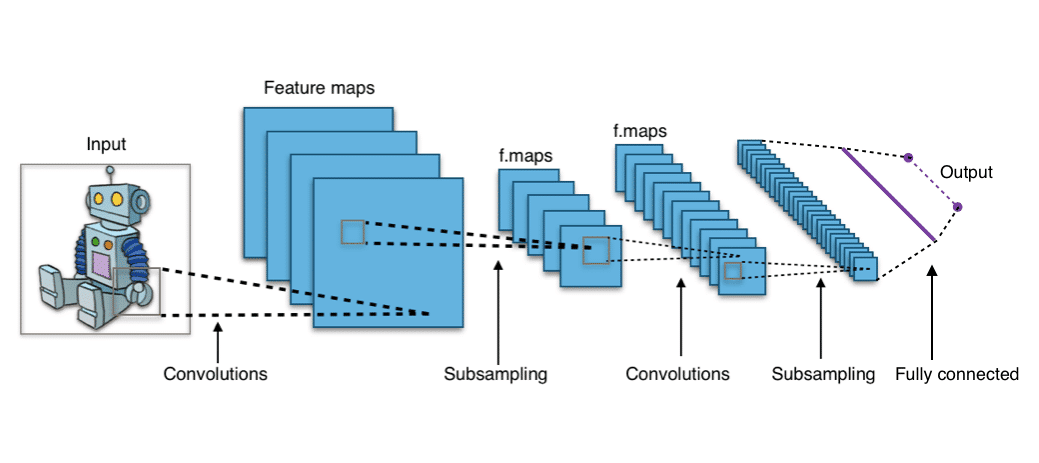
\includegraphics[scale=0.4]{CNN4.png}
    \caption{Convolutional Neural Network}
\end{figure}

\section{CNNs vs Feed-forward Neural Nets!}
    An image is nothing but a matrix of pixel values, right? So why not just flatten the image (e.g. 3x3 image matrix into a 9x1 vector) and feed it to a Multi-Level Perceptron for classification purposes?
\\ \\
    In cases of extremely basic binary images, the method might show an average precision score while performing prediction of classes but would have little to no accuracy when it comes to complex images having pixel dependencies throughout.
\\ \\
    A ConvNet is able to successfully capture the Spatial and Temporal dependencies in an image through the application of relevant filters. The architecture performs a better fitting to the image dataset due to the reduction in the number of parameters involved and the reusability of weights. In other words, the network can be trained to understand the sophistication of the image better.

\section{Convolution Layer — The Kernel}
    Each convolutional layer contains a series of filters known as convolutional kernels. The filter is a matrix of integers that are used on a subset of the input pixel values, the same size as the kernel. Each pixel is multiplied by the corresponding value in the kernel, then the result is summed up for a single value for simplicity representing a grid cell, like a pixel, in the output channel/feature map. These are linear transformations, each convolution is a type of affine function.

    \begin{figure}[h]
        \centering
        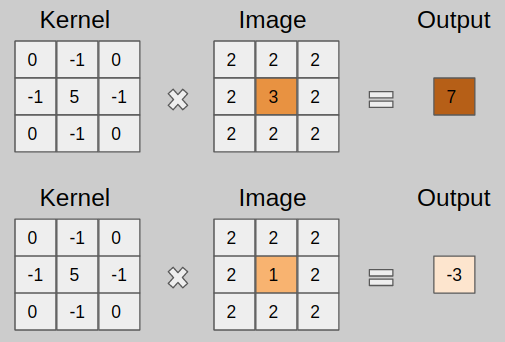
\includegraphics[scale=0.4]{CNN3.png}
        \caption{Average and Max pooling layer}
    \end{figure}

    In computer vision, the input is often a 3 channel RGB image. For simplicity, if we take a greyscale image that has one channel (a two-dimensional matrix) and a 3x3 convolutional kernel (a two-dimensional matrix). The kernel strides over the input matrix of numbers moving horizontally column by column, sliding/scanning over the first rows in the matrix containing the images pixel values. Then the kernel strides down vertically to subsequent rows. Note, the filter may stride over one or several pixels at a time, this is detailed further below. In other non-vision applications, a one-dimensional convolution may slide vertically over an input matrix.

\section{Pooling Layer}
    Similar to the Convolutional Layer, the Pooling layer is responsible for reducing the spatial size of the Convolved Feature. This is to decrease the computational power required to process the data through dimensionality reduction. Furthermore, it is useful for extracting dominant features that are rotational and positional invariant, thus maintaining the process of effectively training of the model.
\\ \\
    There are two types of Pooling: Max Pooling and Average Pooling. Max Pooling returns the maximum value from the portion of the image covered by the Kernel. On the other hand, Average Pooling returns the average of all the values from the portion of the image covered by the Kernel.

    \begin{figure}[h]
        \centering
        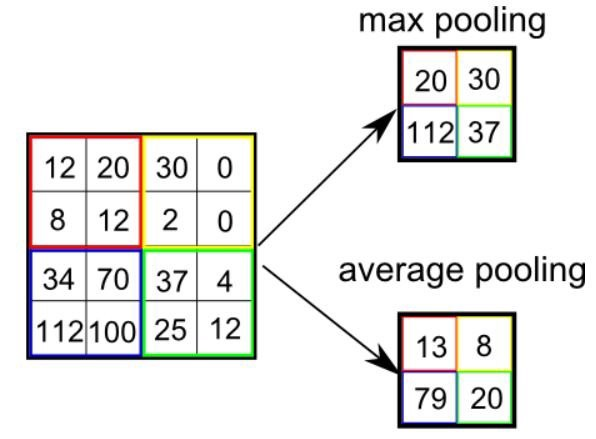
\includegraphics[scale=0.4]{CNN1.jpeg}
        \caption{Average and Max pooling layer}
    \end{figure}

    Max Pooling also performs as a Noise Suppressant. It discards the noisy activations altogether and also performs de-noising along with dimensionality reduction. On the other hand, Average Pooling simply performs dimensionality reduction as a noise suppressing mechanism. Hence, we can say that Max Pooling performs a lot better than Average Pooling.
\\ \\
    The Convolutional Layer and the Pooling Layer, together form the i-th layer of a Convolutional Neural Network. Depending on the complexities in the images, the number of such layers may be increased for capturing low-levels details even further, but at the cost of more computational power.
\\ \\
    After going through the above process, we have successfully enabled the model to understand the features. Moving on, we are going to flatten the final output and feed it to a regular Neural Network for classification purposes.

  \newpage

  \section{Style Transfer}
  Neural style transfer is an optimization technique used to take two images—a content image and a style reference image (such as an artwork by a famous painter) and blend them together so the output image looks like the content image, but “painted” in the style of the style reference image.
      \begin{tcolorbox}[breakable, size=fbox, boxrule=1pt, pad at break*=1mm,colback=cellbackground, colframe=cellborder]
\prompt{In}{incolor}{0}{\boxspacing}
\begin{Verbatim}[commandchars=\\\{\}]
\PY{o}{!}pip install torch torchvision
\PY{o}{!}pip install \PY{n+nv}{Pillow}\PY{o}{=}\PY{o}{=}\PY{l+m}{4}.0.0
\end{Verbatim}
\end{tcolorbox}  
    
    \begin{tcolorbox}[breakable, size=fbox, boxrule=1pt, pad at break*=1mm,colback=cellbackground, colframe=cellborder]
\prompt{In}{incolor}{1}{\boxspacing}
\begin{Verbatim}[commandchars=\\\{\}]
\PY{o}{\PYZpc{}}\PY{k}{matplotlib} inline
\PY{k+kn}{import} \PY{n+nn}{torch}
\PY{k+kn}{import} \PY{n+nn}{torch}\PY{n+nn}{.}\PY{n+nn}{optim} \PY{k}{as} \PY{n+nn}{optim}
\PY{k+kn}{from} \PY{n+nn}{torchvision} \PY{k+kn}{import} \PY{n}{transforms}\PY{p}{,} \PY{n}{models}
\PY{k+kn}{from} \PY{n+nn}{PIL} \PY{k+kn}{import} \PY{n}{Image}
\PY{k+kn}{import} \PY{n+nn}{matplotlib}\PY{n+nn}{.}\PY{n+nn}{pyplot} \PY{k}{as} \PY{n+nn}{plt}
\PY{k+kn}{import} \PY{n+nn}{numpy} \PY{k}{as} \PY{n+nn}{np}
\end{Verbatim}
\end{tcolorbox}

    \begin{tcolorbox}[breakable, size=fbox, boxrule=1pt, pad at break*=1mm,colback=cellbackground, colframe=cellborder]
\prompt{In}{incolor}{2}{\boxspacing}
\begin{Verbatim}[commandchars=\\\{\}]
\PY{n}{vgg} \PY{o}{=} \PY{n}{models}\PY{o}{.}\PY{n}{vgg19}\PY{p}{(}\PY{n}{pretrained}\PY{o}{=}\PY{k+kc}{True}\PY{p}{)}\PY{o}{.}\PY{n}{features}

\PY{k}{for} \PY{n}{params} \PY{o+ow}{in} \PY{n}{vgg}\PY{o}{.}\PY{n}{parameters}\PY{p}{(}\PY{p}{)}\PY{p}{:}
    \PY{n}{params}\PY{o}{.}\PY{n}{requires\PYZus{}grad\PYZus{}}\PY{p}{(}\PY{k+kc}{False}\PY{p}{)}
\end{Verbatim}
\end{tcolorbox}

    \begin{Verbatim}[commandchars=\\\{\}]
Downloading: "https://download.pytorch.org/models/vgg19-dcbb9e9d.pth" to
/home/sahasra/.cache/torch/checkpoints/vgg19-dcbb9e9d.pth
    \end{Verbatim}

    
    \begin{verbatim}
HBox(children=(FloatProgress(value=0.0, max=574673361.0), HTML(value='')))
    \end{verbatim}

    
    \begin{Verbatim}[commandchars=\\\{\}]

    \end{Verbatim}

    \begin{tcolorbox}[breakable, size=fbox, boxrule=1pt, pad at break*=1mm,colback=cellbackground, colframe=cellborder]
\prompt{In}{incolor}{3}{\boxspacing}
\begin{Verbatim}[commandchars=\\\{\}]
\PY{n}{device} \PY{o}{=} \PY{n}{torch}\PY{o}{.}\PY{n}{device}\PY{p}{(}\PY{l+s+s1}{\PYZsq{}}\PY{l+s+s1}{CUDA}\PY{l+s+s1}{\PYZsq{}} \PY{k}{if} \PY{n}{torch}\PY{o}{.}\PY{n}{cuda}\PY{o}{.}\PY{n}{is\PYZus{}available}\PY{p}{(}\PY{p}{)} \PY{k}{else} \PY{l+s+s1}{\PYZsq{}}\PY{l+s+s1}{cpu}\PY{l+s+s1}{\PYZsq{}}\PY{p}{)}
\PY{n}{vgg}\PY{o}{.}\PY{n}{to}\PY{p}{(}\PY{n}{device}\PY{p}{)}
\end{Verbatim}
\end{tcolorbox}

            \begin{tcolorbox}[breakable, size=fbox, boxrule=.5pt, pad at break*=1mm, opacityfill=0]
\prompt{Out}{outcolor}{3}{\boxspacing}
\begin{Verbatim}[commandchars=\\\{\}]
Sequential(
  (0): Conv2d(3, 64, kernel\_size=(3, 3), stride=(1, 1), padding=(1, 1))
  (1): ReLU(inplace=True)
  (2): Conv2d(64, 64, kernel\_size=(3, 3), stride=(1, 1), padding=(1, 1))
  (3): ReLU(inplace=True)
  (4): MaxPool2d(kernel\_size=2, stride=2, padding=0, dilation=1,
ceil\_mode=False)
  (5): Conv2d(64, 128, kernel\_size=(3, 3), stride=(1, 1), padding=(1, 1))
  (6): ReLU(inplace=True)
  (7): Conv2d(128, 128, kernel\_size=(3, 3), stride=(1, 1), padding=(1, 1))
  (8): ReLU(inplace=True)
  (9): MaxPool2d(kernel\_size=2, stride=2, padding=0, dilation=1,
ceil\_mode=False)
  (10): Conv2d(128, 256, kernel\_size=(3, 3), stride=(1, 1), padding=(1, 1))
  (11): ReLU(inplace=True)
  (12): Conv2d(256, 256, kernel\_size=(3, 3), stride=(1, 1), padding=(1, 1))
  (13): ReLU(inplace=True)
  (14): Conv2d(256, 256, kernel\_size=(3, 3), stride=(1, 1), padding=(1, 1))
  (15): ReLU(inplace=True)
  (16): Conv2d(256, 256, kernel\_size=(3, 3), stride=(1, 1), padding=(1, 1))
  (17): ReLU(inplace=True)
  (18): MaxPool2d(kernel\_size=2, stride=2, padding=0, dilation=1,
ceil\_mode=False)
  (19): Conv2d(256, 512, kernel\_size=(3, 3), stride=(1, 1), padding=(1, 1))
  (20): ReLU(inplace=True)
  (21): Conv2d(512, 512, kernel\_size=(3, 3), stride=(1, 1), padding=(1, 1))
  (22): ReLU(inplace=True)
  (23): Conv2d(512, 512, kernel\_size=(3, 3), stride=(1, 1), padding=(1, 1))
  (24): ReLU(inplace=True)
  (25): Conv2d(512, 512, kernel\_size=(3, 3), stride=(1, 1), padding=(1, 1))
  (26): ReLU(inplace=True)
  (27): MaxPool2d(kernel\_size=2, stride=2, padding=0, dilation=1,
ceil\_mode=False)
  (28): Conv2d(512, 512, kernel\_size=(3, 3), stride=(1, 1), padding=(1, 1))
  (29): ReLU(inplace=True)
  (30): Conv2d(512, 512, kernel\_size=(3, 3), stride=(1, 1), padding=(1, 1))
  (31): ReLU(inplace=True)
  (32): Conv2d(512, 512, kernel\_size=(3, 3), stride=(1, 1), padding=(1, 1))
  (33): ReLU(inplace=True)
  (34): Conv2d(512, 512, kernel\_size=(3, 3), stride=(1, 1), padding=(1, 1))
  (35): ReLU(inplace=True)
  (36): MaxPool2d(kernel\_size=2, stride=2, padding=0, dilation=1,
ceil\_mode=False)
)
\end{Verbatim}
\end{tcolorbox}
        
    \begin{tcolorbox}[breakable, size=fbox, boxrule=1pt, pad at break*=1mm,colback=cellbackground, colframe=cellborder]
\prompt{In}{incolor}{4}{\boxspacing}
\begin{Verbatim}[commandchars=\\\{\}]
\PY{k}{def} \PY{n+nf}{load\PYZus{}image}\PY{p}{(}\PY{n}{img\PYZus{}path}\PY{p}{,} \PY{n}{max\PYZus{}size}\PY{o}{=}\PY{l+m+mi}{400}\PY{p}{,} \PY{n}{shape}\PY{o}{=}\PY{k+kc}{None}\PY{p}{)}\PY{p}{:}
    
    \PY{n}{image} \PY{o}{=} \PY{n}{Image}\PY{o}{.}\PY{n}{open}\PY{p}{(}\PY{n}{img\PYZus{}path}\PY{p}{)}\PY{o}{.}\PY{n}{convert}\PY{p}{(}\PY{l+s+s1}{\PYZsq{}}\PY{l+s+s1}{RGB}\PY{l+s+s1}{\PYZsq{}}\PY{p}{)}
    \PY{k}{if} \PY{n+nb}{max}\PY{p}{(}\PY{n}{image}\PY{o}{.}\PY{n}{size}\PY{p}{)} \PY{o}{\PYZgt{}} \PY{n}{max\PYZus{}size}\PY{p}{:}
        \PY{n}{size} \PY{o}{=} \PY{n}{max\PYZus{}size}
    \PY{k}{else}\PY{p}{:}
        \PY{n}{size} \PY{o}{=} \PY{n+nb}{max}\PY{p}{(}\PY{n}{image}\PY{o}{.}\PY{n}{size}\PY{p}{)}
    
    \PY{k}{if} \PY{n}{shape} \PY{o+ow}{is} \PY{o+ow}{not} \PY{k+kc}{None}\PY{p}{:}
        \PY{n}{size} \PY{o}{=} \PY{n}{shape}
 
    \PY{n}{in\PYZus{}transform} \PY{o}{=} \PY{n}{transforms}\PY{o}{.}\PY{n}{Compose}\PY{p}{(}\PY{p}{[}
                        \PY{n}{transforms}\PY{o}{.}\PY{n}{Resize}\PY{p}{(}\PY{n}{size}\PY{p}{)}\PY{p}{,}
                        \PY{n}{transforms}\PY{o}{.}\PY{n}{ToTensor}\PY{p}{(}\PY{p}{)}\PY{p}{,}
                        \PY{n}{transforms}\PY{o}{.}\PY{n}{Normalize}\PY{p}{(}\PY{p}{(}\PY{l+m+mf}{0.5}\PY{p}{,} \PY{l+m+mf}{0.5}\PY{p}{,} \PY{l+m+mf}{0.5}\PY{p}{)}\PY{p}{,} 
                                             \PY{p}{(}\PY{l+m+mf}{0.5}\PY{p}{,} \PY{l+m+mf}{0.5}\PY{p}{,} \PY{l+m+mf}{0.5}\PY{p}{)}\PY{p}{)}\PY{p}{]}\PY{p}{)}

    \PY{n}{image} \PY{o}{=} \PY{n}{in\PYZus{}transform}\PY{p}{(}\PY{n}{image}\PY{p}{)}\PY{o}{.}\PY{n}{unsqueeze}\PY{p}{(}\PY{l+m+mi}{0}\PY{p}{)}
    
    \PY{k}{return} \PY{n}{image}
\end{Verbatim}
\end{tcolorbox}

    \begin{tcolorbox}[breakable, size=fbox, boxrule=1pt, pad at break*=1mm,colback=cellbackground, colframe=cellborder]
\prompt{In}{incolor}{6}{\boxspacing}
\begin{Verbatim}[commandchars=\\\{\}]
\PY{n}{content} \PY{o}{=} \PY{n}{load\PYZus{}image}\PY{p}{(}\PY{l+s+s1}{\PYZsq{}}\PY{l+s+s1}{./data/styleTransfer\PYZhy{}1/Images/City.jpg}\PY{l+s+s1}{\PYZsq{}}\PY{p}{)}\PY{o}{.}\PY{n}{to}\PY{p}{(}\PY{n}{device}\PY{p}{)}
\PY{n}{style} \PY{o}{=} \PY{n}{load\PYZus{}image}\PY{p}{(}\PY{l+s+s1}{\PYZsq{}}\PY{l+s+s1}{./data/styleTransfer\PYZhy{}1/Images/StarryNight.jpg}\PY{l+s+s1}{\PYZsq{}}\PY{p}{,} \PY{n}{shape}\PY{o}{=}\PY{n}{content}\PY{o}{.}\PY{n}{shape}\PY{p}{[}\PY{o}{\PYZhy{}}\PY{l+m+mi}{2}\PY{p}{:}\PY{p}{]}\PY{p}{)}\PY{o}{.}\PY{n}{to}\PY{p}{(}\PY{n}{device}\PY{p}{)}
\end{Verbatim}
\end{tcolorbox}

    \begin{tcolorbox}[breakable, size=fbox, boxrule=1pt, pad at break*=1mm,colback=cellbackground, colframe=cellborder]
\prompt{In}{incolor}{7}{\boxspacing}
\begin{Verbatim}[commandchars=\\\{\}]
\PY{k}{def} \PY{n+nf}{im\PYZus{}convert}\PY{p}{(}\PY{n}{tensor}\PY{p}{)}\PY{p}{:}
    \PY{n}{image} \PY{o}{=} \PY{n}{tensor}\PY{o}{.}\PY{n}{to}\PY{p}{(}\PY{l+s+s2}{\PYZdq{}}\PY{l+s+s2}{cpu}\PY{l+s+s2}{\PYZdq{}}\PY{p}{)}\PY{o}{.}\PY{n}{clone}\PY{p}{(}\PY{p}{)}\PY{o}{.}\PY{n}{detach}\PY{p}{(}\PY{p}{)}
    \PY{n}{image} \PY{o}{=} \PY{n}{image}\PY{o}{.}\PY{n}{numpy}\PY{p}{(}\PY{p}{)}\PY{o}{.}\PY{n}{squeeze}\PY{p}{(}\PY{p}{)}
    \PY{n}{image} \PY{o}{=} \PY{n}{image}\PY{o}{.}\PY{n}{transpose}\PY{p}{(}\PY{l+m+mi}{1}\PY{p}{,}\PY{l+m+mi}{2}\PY{p}{,}\PY{l+m+mi}{0}\PY{p}{)}
    \PY{n}{image} \PY{o}{=} \PY{n}{image} \PY{o}{*} \PY{n}{np}\PY{o}{.}\PY{n}{array}\PY{p}{(}\PY{p}{(}\PY{l+m+mf}{0.5}\PY{p}{,} \PY{l+m+mf}{0.5}\PY{p}{,} \PY{l+m+mf}{0.5}\PY{p}{)}\PY{p}{)} \PY{o}{+} \PY{n}{np}\PY{o}{.}\PY{n}{array}\PY{p}{(}\PY{p}{(}\PY{l+m+mf}{0.5}\PY{p}{,} \PY{l+m+mf}{0.5}\PY{p}{,} \PY{l+m+mf}{0.5}\PY{p}{)}\PY{p}{)}
    \PY{n}{image} \PY{o}{=} \PY{n}{image}\PY{o}{.}\PY{n}{clip}\PY{p}{(}\PY{l+m+mi}{0}\PY{p}{,} \PY{l+m+mi}{1}\PY{p}{)}

    \PY{k}{return} \PY{n}{image}
\end{Verbatim}
\end{tcolorbox}

    \begin{tcolorbox}[breakable, size=fbox, boxrule=1pt, pad at break*=1mm,colback=cellbackground, colframe=cellborder]
\prompt{In}{incolor}{8}{\boxspacing}
\begin{Verbatim}[commandchars=\\\{\}]
\PY{n}{fig}\PY{p}{,} \PY{p}{(}\PY{n}{ax1}\PY{p}{,} \PY{n}{ax2}\PY{p}{)} \PY{o}{=} \PY{n}{plt}\PY{o}{.}\PY{n}{subplots}\PY{p}{(}\PY{l+m+mi}{1}\PY{p}{,} \PY{l+m+mi}{2}\PY{p}{,} \PY{n}{figsize}\PY{o}{=}\PY{p}{(}\PY{l+m+mi}{20}\PY{p}{,}\PY{l+m+mi}{10}\PY{p}{)}\PY{p}{)}
\PY{n}{ax1}\PY{o}{.}\PY{n}{imshow}\PY{p}{(}\PY{n}{im\PYZus{}convert}\PY{p}{(}\PY{n}{content}\PY{p}{)}\PY{p}{)}
\PY{n}{ax1}\PY{o}{.}\PY{n}{axis}\PY{p}{(}\PY{l+s+s1}{\PYZsq{}}\PY{l+s+s1}{off}\PY{l+s+s1}{\PYZsq{}}\PY{p}{)}
\PY{n}{ax2}\PY{o}{.}\PY{n}{imshow}\PY{p}{(}\PY{n}{im\PYZus{}convert}\PY{p}{(}\PY{n}{style}\PY{p}{)}\PY{p}{)}
\PY{n}{ax2}\PY{o}{.}\PY{n}{axis}\PY{p}{(}\PY{l+s+s1}{\PYZsq{}}\PY{l+s+s1}{off}\PY{l+s+s1}{\PYZsq{}}\PY{p}{)}
\end{Verbatim}
\end{tcolorbox}

            \begin{tcolorbox}[breakable, size=fbox, boxrule=.5pt, pad at break*=1mm, opacityfill=0]
\prompt{Out}{outcolor}{8}{\boxspacing}
\begin{Verbatim}[commandchars=\\\{\}]
(-0.5, 599.5, 399.5, -0.5)
\end{Verbatim}
\end{tcolorbox}
        
    \begin{center}
    \adjustimage{max size={0.9\linewidth}{0.9\paperheight}}{Style Transfer_files/Style Transfer_7_1.png}
    \end{center}
    { \hspace*{\fill} \\}
    
    \begin{tcolorbox}[breakable, size=fbox, boxrule=1pt, pad at break*=1mm,colback=cellbackground, colframe=cellborder]
\prompt{In}{incolor}{9}{\boxspacing}
\begin{Verbatim}[commandchars=\\\{\}]
\PY{k}{def} \PY{n+nf}{get\PYZus{}features}\PY{p}{(}\PY{n}{image}\PY{p}{,} \PY{n}{model}\PY{p}{)}\PY{p}{:}
   
    \PY{n}{layers} \PY{o}{=} \PY{p}{\PYZob{}}\PY{l+s+s1}{\PYZsq{}}\PY{l+s+s1}{0}\PY{l+s+s1}{\PYZsq{}}\PY{p}{:} \PY{l+s+s1}{\PYZsq{}}\PY{l+s+s1}{conv1\PYZus{}1}\PY{l+s+s1}{\PYZsq{}}\PY{p}{,}
              \PY{l+s+s1}{\PYZsq{}}\PY{l+s+s1}{5}\PY{l+s+s1}{\PYZsq{}}\PY{p}{:} \PY{l+s+s1}{\PYZsq{}}\PY{l+s+s1}{conv2\PYZus{}1}\PY{l+s+s1}{\PYZsq{}}\PY{p}{,} 
              \PY{l+s+s1}{\PYZsq{}}\PY{l+s+s1}{10}\PY{l+s+s1}{\PYZsq{}}\PY{p}{:} \PY{l+s+s1}{\PYZsq{}}\PY{l+s+s1}{conv3\PYZus{}1}\PY{l+s+s1}{\PYZsq{}}\PY{p}{,} 
              \PY{l+s+s1}{\PYZsq{}}\PY{l+s+s1}{19}\PY{l+s+s1}{\PYZsq{}}\PY{p}{:} \PY{l+s+s1}{\PYZsq{}}\PY{l+s+s1}{conv4\PYZus{}1}\PY{l+s+s1}{\PYZsq{}}\PY{p}{,}
              \PY{l+s+s1}{\PYZsq{}}\PY{l+s+s1}{21}\PY{l+s+s1}{\PYZsq{}}\PY{p}{:} \PY{l+s+s1}{\PYZsq{}}\PY{l+s+s1}{conv4\PYZus{}2}\PY{l+s+s1}{\PYZsq{}}\PY{p}{,}  \PY{c+c1}{\PYZsh{} Content Extraction}
              \PY{l+s+s1}{\PYZsq{}}\PY{l+s+s1}{28}\PY{l+s+s1}{\PYZsq{}}\PY{p}{:} \PY{l+s+s1}{\PYZsq{}}\PY{l+s+s1}{conv5\PYZus{}1}\PY{l+s+s1}{\PYZsq{}}\PY{p}{\PYZcb{}}
        
    \PY{n}{features} \PY{o}{=} \PY{p}{\PYZob{}}\PY{p}{\PYZcb{}}

    \PY{k}{for} \PY{n}{name}\PY{p}{,} \PY{n}{layer} \PY{o+ow}{in} \PY{n}{model}\PY{o}{.}\PY{n}{\PYZus{}modules}\PY{o}{.}\PY{n}{items}\PY{p}{(}\PY{p}{)}\PY{p}{:}
        \PY{n}{image} \PY{o}{=} \PY{n}{layer}\PY{p}{(}\PY{n}{image}\PY{p}{)}
        \PY{k}{if} \PY{n}{name} \PY{o+ow}{in} \PY{n}{layers}\PY{p}{:}
            \PY{n}{features}\PY{p}{[}\PY{n}{layers}\PY{p}{[}\PY{n}{name}\PY{p}{]}\PY{p}{]} \PY{o}{=} \PY{n}{image}
            
    \PY{k}{return} \PY{n}{features}
\end{Verbatim}
\end{tcolorbox}

    \begin{tcolorbox}[breakable, size=fbox, boxrule=1pt, pad at break*=1mm,colback=cellbackground, colframe=cellborder]
\prompt{In}{incolor}{10}{\boxspacing}
\begin{Verbatim}[commandchars=\\\{\}]
\PY{n}{content\PYZus{}features} \PY{o}{=} \PY{n}{get\PYZus{}features}\PY{p}{(}\PY{n}{content}\PY{p}{,} \PY{n}{vgg}\PY{p}{)}
\PY{n}{style\PYZus{}features} \PY{o}{=} \PY{n}{get\PYZus{}features}\PY{p}{(}\PY{n}{style}\PY{p}{,} \PY{n}{vgg}\PY{p}{)}
\end{Verbatim}
\end{tcolorbox}

    \begin{tcolorbox}[breakable, size=fbox, boxrule=1pt, pad at break*=1mm,colback=cellbackground, colframe=cellborder]
\prompt{In}{incolor}{11}{\boxspacing}
\begin{Verbatim}[commandchars=\\\{\}]
\PY{k}{def} \PY{n+nf}{gram\PYZus{}matrix}\PY{p}{(}\PY{n}{tensor}\PY{p}{)}\PY{p}{:}
  \PY{n}{\PYZus{}}\PY{p}{,} \PY{n}{d}\PY{p}{,} \PY{n}{h}\PY{p}{,} \PY{n}{w} \PY{o}{=} \PY{n}{tensor}\PY{o}{.}\PY{n}{size}\PY{p}{(}\PY{p}{)}
  \PY{n}{tensor} \PY{o}{=} \PY{n}{tensor}\PY{o}{.}\PY{n}{view}\PY{p}{(}\PY{n}{d}\PY{p}{,} \PY{n}{h} \PY{o}{*} \PY{n}{w}\PY{p}{)}
  \PY{n}{gram} \PY{o}{=} \PY{n}{torch}\PY{o}{.}\PY{n}{mm}\PY{p}{(}\PY{n}{tensor}\PY{p}{,} \PY{n}{tensor}\PY{o}{.}\PY{n}{t}\PY{p}{(}\PY{p}{)}\PY{p}{)}
  \PY{k}{return} \PY{n}{gram}
\end{Verbatim}
\end{tcolorbox}

    \begin{tcolorbox}[breakable, size=fbox, boxrule=1pt, pad at break*=1mm,colback=cellbackground, colframe=cellborder]
\prompt{In}{incolor}{12}{\boxspacing}
\begin{Verbatim}[commandchars=\\\{\}]
\PY{n}{style\PYZus{}grams} \PY{o}{=} \PY{p}{\PYZob{}}\PY{n}{layer}\PY{p}{:} \PY{n}{gram\PYZus{}matrix}\PY{p}{(}\PY{n}{style\PYZus{}features}\PY{p}{[}\PY{n}{layer}\PY{p}{]}\PY{p}{)} \PY{k}{for} \PY{n}{layer} \PY{o+ow}{in} \PY{n}{style\PYZus{}features}\PY{p}{\PYZcb{}}
\end{Verbatim}
\end{tcolorbox}

    \begin{tcolorbox}[breakable, size=fbox, boxrule=1pt, pad at break*=1mm,colback=cellbackground, colframe=cellborder]
\prompt{In}{incolor}{13}{\boxspacing}
\begin{Verbatim}[commandchars=\\\{\}]
\PY{n}{style\PYZus{}weights} \PY{o}{=} \PY{p}{\PYZob{}}\PY{l+s+s1}{\PYZsq{}}\PY{l+s+s1}{conv1\PYZus{}1}\PY{l+s+s1}{\PYZsq{}}\PY{p}{:} \PY{l+m+mf}{1.}\PY{p}{,}
                 \PY{l+s+s1}{\PYZsq{}}\PY{l+s+s1}{conv2\PYZus{}1}\PY{l+s+s1}{\PYZsq{}}\PY{p}{:} \PY{l+m+mf}{0.75}\PY{p}{,}
                 \PY{l+s+s1}{\PYZsq{}}\PY{l+s+s1}{conv3\PYZus{}1}\PY{l+s+s1}{\PYZsq{}}\PY{p}{:} \PY{l+m+mf}{0.2}\PY{p}{,}
                 \PY{l+s+s1}{\PYZsq{}}\PY{l+s+s1}{conv4\PYZus{}1}\PY{l+s+s1}{\PYZsq{}}\PY{p}{:} \PY{l+m+mf}{0.2}\PY{p}{,}
                 \PY{l+s+s1}{\PYZsq{}}\PY{l+s+s1}{conv5\PYZus{}1}\PY{l+s+s1}{\PYZsq{}}\PY{p}{:} \PY{l+m+mf}{0.2}\PY{p}{\PYZcb{}}

\PY{n}{content\PYZus{}weight} \PY{o}{=} \PY{l+m+mi}{1}  \PY{c+c1}{\PYZsh{} alpha}
\PY{n}{style\PYZus{}weight} \PY{o}{=} \PY{l+m+mf}{1e6}  \PY{c+c1}{\PYZsh{} beta}
\end{Verbatim}
\end{tcolorbox}

    \begin{tcolorbox}[breakable, size=fbox, boxrule=1pt, pad at break*=1mm,colback=cellbackground, colframe=cellborder]
\prompt{In}{incolor}{14}{\boxspacing}
\begin{Verbatim}[commandchars=\\\{\}]
\PY{n}{target} \PY{o}{=} \PY{n}{content}\PY{o}{.}\PY{n}{clone}\PY{p}{(}\PY{p}{)}\PY{o}{.}\PY{n}{requires\PYZus{}grad\PYZus{}}\PY{p}{(}\PY{k+kc}{True}\PY{p}{)}\PY{o}{.}\PY{n}{to}\PY{p}{(}\PY{n}{device}\PY{p}{)}
\end{Verbatim}
\end{tcolorbox}

    \begin{tcolorbox}[breakable, size=fbox, boxrule=1pt, pad at break*=1mm,colback=cellbackground, colframe=cellborder]
\prompt{In}{incolor}{15}{\boxspacing}
\begin{Verbatim}[commandchars=\\\{\}]
\PY{n}{show\PYZus{}every} \PY{o}{=} \PY{l+m+mi}{300}
\PY{n}{optimizer} \PY{o}{=} \PY{n}{optim}\PY{o}{.}\PY{n}{Adam}\PY{p}{(}\PY{p}{[}\PY{n}{target}\PY{p}{]}\PY{p}{,} \PY{n}{lr}\PY{o}{=}\PY{l+m+mf}{0.003}\PY{p}{)}
\PY{n}{steps} \PY{o}{=} \PY{l+m+mi}{2100}

\PY{n}{height}\PY{p}{,} \PY{n}{width}\PY{p}{,} \PY{n}{channels} \PY{o}{=} \PY{n}{im\PYZus{}convert}\PY{p}{(}\PY{n}{target}\PY{p}{)}\PY{o}{.}\PY{n}{shape}
\PY{n}{image\PYZus{}array} \PY{o}{=} \PY{n}{np}\PY{o}{.}\PY{n}{empty}\PY{p}{(}\PY{n}{shape}\PY{o}{=}\PY{p}{(}\PY{l+m+mi}{300}\PY{p}{,} \PY{n}{height}\PY{p}{,} \PY{n}{width}\PY{p}{,} \PY{n}{channels}\PY{p}{)}\PY{p}{)}
\PY{n}{capture\PYZus{}frame} \PY{o}{=} \PY{n}{steps}\PY{o}{/}\PY{l+m+mi}{300}
\PY{n}{counter} \PY{o}{=} \PY{l+m+mi}{0}
\end{Verbatim}
\end{tcolorbox}

    \begin{tcolorbox}[breakable, size=fbox, boxrule=1pt, pad at break*=1mm,colback=cellbackground, colframe=cellborder]
\prompt{In}{incolor}{17}{\boxspacing}
\begin{Verbatim}[commandchars=\\\{\}]
\PY{k}{for} \PY{n}{ii} \PY{o+ow}{in} \PY{n+nb}{range}\PY{p}{(}\PY{l+m+mi}{1}\PY{p}{,} \PY{n}{steps}\PY{o}{+}\PY{l+m+mi}{1}\PY{p}{)}\PY{p}{:}
  \PY{n}{target\PYZus{}features} \PY{o}{=} \PY{n}{get\PYZus{}features}\PY{p}{(}\PY{n}{target}\PY{p}{,} \PY{n}{vgg}\PY{p}{)}
  \PY{n}{content\PYZus{}loss} \PY{o}{=} \PY{n}{torch}\PY{o}{.}\PY{n}{mean}\PY{p}{(}\PY{p}{(}\PY{n}{target\PYZus{}features}\PY{p}{[}\PY{l+s+s1}{\PYZsq{}}\PY{l+s+s1}{conv4\PYZus{}2}\PY{l+s+s1}{\PYZsq{}}\PY{p}{]} \PY{o}{\PYZhy{}} \PY{n}{content\PYZus{}features}\PY{p}{[}\PY{l+s+s1}{\PYZsq{}}\PY{l+s+s1}{conv4\PYZus{}2}\PY{l+s+s1}{\PYZsq{}}\PY{p}{]}\PY{p}{)}\PY{o}{*}\PY{o}{*}\PY{l+m+mi}{2}\PY{p}{)}
  \PY{n}{style\PYZus{}loss} \PY{o}{=} \PY{l+m+mi}{0}

  \PY{k}{for} \PY{n}{layer} \PY{o+ow}{in} \PY{n}{style\PYZus{}weights}\PY{p}{:}
    \PY{n}{target\PYZus{}feature} \PY{o}{=} \PY{n}{target\PYZus{}features}\PY{p}{[}\PY{n}{layer}\PY{p}{]}
    \PY{n}{target\PYZus{}gram} \PY{o}{=} \PY{n}{gram\PYZus{}matrix}\PY{p}{(}\PY{n}{target\PYZus{}feature}\PY{p}{)}
    \PY{n}{style\PYZus{}gram} \PY{o}{=} \PY{n}{style\PYZus{}grams}\PY{p}{[}\PY{n}{layer}\PY{p}{]}
    \PY{n}{layer\PYZus{}style\PYZus{}loss} \PY{o}{=} \PY{n}{style\PYZus{}weights}\PY{p}{[}\PY{n}{layer}\PY{p}{]} \PY{o}{*} \PY{n}{torch}\PY{o}{.}\PY{n}{mean}\PY{p}{(}\PY{p}{(}\PY{n}{target\PYZus{}gram} \PY{o}{\PYZhy{}} \PY{n}{style\PYZus{}gram}\PY{p}{)}\PY{o}{*}\PY{o}{*}\PY{l+m+mi}{2}\PY{p}{)}
    \PY{n}{\PYZus{}}\PY{p}{,} \PY{n}{d}\PY{p}{,} \PY{n}{h}\PY{p}{,} \PY{n}{w} \PY{o}{=} \PY{n}{target\PYZus{}feature}\PY{o}{.}\PY{n}{shape}
    \PY{n}{style\PYZus{}loss} \PY{o}{+}\PY{o}{=} \PY{n}{layer\PYZus{}style\PYZus{}loss} \PY{o}{/} \PY{p}{(}\PY{n}{d}\PY{o}{*}\PY{n}{h}\PY{o}{*}\PY{n}{w}\PY{p}{)}

  \PY{n}{total\PYZus{}loss} \PY{o}{=} \PY{n}{content\PYZus{}weight}\PY{o}{*}\PY{n}{content\PYZus{}loss} \PY{o}{+} \PY{n}{style\PYZus{}weight}\PY{o}{*}\PY{n}{style\PYZus{}loss}

  \PY{n}{optimizer}\PY{o}{.}\PY{n}{zero\PYZus{}grad}\PY{p}{(}\PY{p}{)}
  \PY{n}{total\PYZus{}loss}\PY{o}{.}\PY{n}{backward}\PY{p}{(}\PY{p}{)}
  \PY{n}{optimizer}\PY{o}{.}\PY{n}{step}\PY{p}{(}\PY{p}{)}

  \PY{k}{if} \PY{n}{ii} \PY{o}{\PYZpc{}} \PY{n}{show\PYZus{}every} \PY{o}{==} \PY{l+m+mi}{0}\PY{p}{:}
    \PY{n+nb}{print}\PY{p}{(}\PY{l+s+s1}{\PYZsq{}}\PY{l+s+s1}{Total loss: }\PY{l+s+s1}{\PYZsq{}}\PY{p}{,} \PY{n}{total\PYZus{}loss}\PY{o}{.}\PY{n}{item}\PY{p}{(}\PY{p}{)}\PY{p}{)}
    \PY{n+nb}{print}\PY{p}{(}\PY{l+s+s1}{\PYZsq{}}\PY{l+s+s1}{Iteration: }\PY{l+s+s1}{\PYZsq{}}\PY{p}{,} \PY{n}{ii}\PY{p}{)}
    \PY{n}{plt}\PY{o}{.}\PY{n}{imshow}\PY{p}{(}\PY{n}{im\PYZus{}convert}\PY{p}{(}\PY{n}{target}\PY{p}{)}\PY{p}{)}
    \PY{n}{plt}\PY{o}{.}\PY{n}{axis}\PY{p}{(}\PY{l+s+s2}{\PYZdq{}}\PY{l+s+s2}{off}\PY{l+s+s2}{\PYZdq{}}\PY{p}{)}
    \PY{n}{plt}\PY{o}{.}\PY{n}{show}\PY{p}{(}\PY{p}{)}
  
  \PY{k}{if} \PY{n}{ii} \PY{o}{\PYZpc{}} \PY{n}{capture\PYZus{}frame} \PY{o}{==} \PY{l+m+mi}{0}\PY{p}{:}
    \PY{n}{image\PYZus{}array}\PY{p}{[}\PY{n}{counter}\PY{p}{]} \PY{o}{=} \PY{n}{im\PYZus{}convert}\PY{p}{(}\PY{n}{target}\PY{p}{)}
    \PY{n}{counter} \PY{o}{=} \PY{n}{counter} \PY{o}{+} \PY{l+m+mi}{1}
\end{Verbatim}
\end{tcolorbox}

    \begin{Verbatim}[commandchars=\\\{\}]
Total loss:  932833.5
Iteration:  300
    \end{Verbatim}

    \begin{center}
    \adjustimage{max size={0.9\linewidth}{0.9\paperheight}}{Style Transfer_files/Style Transfer_15_1.png}
    \end{center}
    { \hspace*{\fill} \\}
    
    \begin{Verbatim}[commandchars=\\\{\}]
Total loss:  651102.25
Iteration:  600
    \end{Verbatim}

    \begin{center}
    \adjustimage{max size={0.9\linewidth}{0.9\paperheight}}{Style Transfer_files/Style Transfer_15_3.png}
    \end{center}
    { \hspace*{\fill} \\}
    
    \begin{Verbatim}[commandchars=\\\{\}]
Total loss:  504280.59375
Iteration:  900
    \end{Verbatim}

    \begin{center}
    \adjustimage{max size={0.9\linewidth}{0.9\paperheight}}{Style Transfer_files/Style Transfer_15_5.png}
    \end{center}
    { \hspace*{\fill} \\}
    
    \begin{Verbatim}[commandchars=\\\{\}]
Total loss:  395064.53125
Iteration:  1200
    \end{Verbatim}

    \begin{center}
    \adjustimage{max size={0.9\linewidth}{0.9\paperheight}}{Style Transfer_files/Style Transfer_15_7.png}
    \end{center}
    { \hspace*{\fill} \\}
    
    \begin{Verbatim}[commandchars=\\\{\}]
Total loss:  309852.34375
Iteration:  1500
    \end{Verbatim}

    \begin{center}
    \adjustimage{max size={0.9\linewidth}{0.9\paperheight}}{Style Transfer_files/Style Transfer_15_9.png}
    \end{center}
    { \hspace*{\fill} \\}
    
    \begin{Verbatim}[commandchars=\\\{\}]
Total loss:  242368.46875
Iteration:  1800
    \end{Verbatim}

    \begin{center}
    \adjustimage{max size={0.9\linewidth}{0.9\paperheight}}{Style Transfer_files/Style Transfer_15_11.png}
    \end{center}
    { \hspace*{\fill} \\}

    \begin{tcolorbox}[breakable, size=fbox, boxrule=1pt, pad at break*=1mm,colback=cellbackground, colframe=cellborder]
\prompt{In}{incolor}{18}{\boxspacing}
\begin{Verbatim}[commandchars=\\\{\}]
\PY{n}{fig}\PY{p}{,} \PY{p}{(}\PY{n}{ax1}\PY{p}{,} \PY{n}{ax2}\PY{p}{,} \PY{n}{ax3}\PY{p}{)} \PY{o}{=} \PY{n}{plt}\PY{o}{.}\PY{n}{subplots}\PY{p}{(}\PY{l+m+mi}{1}\PY{p}{,} \PY{l+m+mi}{3}\PY{p}{,} \PY{n}{figsize}\PY{o}{=}\PY{p}{(}\PY{l+m+mi}{20}\PY{p}{,} \PY{l+m+mi}{10}\PY{p}{)}\PY{p}{)}
\PY{n}{ax1}\PY{o}{.}\PY{n}{imshow}\PY{p}{(}\PY{n}{im\PYZus{}convert}\PY{p}{(}\PY{n}{content}\PY{p}{)}\PY{p}{)}
\PY{n}{ax1}\PY{o}{.}\PY{n}{axis}\PY{p}{(}\PY{l+s+s1}{\PYZsq{}}\PY{l+s+s1}{off}\PY{l+s+s1}{\PYZsq{}}\PY{p}{)}
\PY{n}{ax2}\PY{o}{.}\PY{n}{imshow}\PY{p}{(}\PY{n}{im\PYZus{}convert}\PY{p}{(}\PY{n}{style}\PY{p}{)}\PY{p}{)}
\PY{n}{ax2}\PY{o}{.}\PY{n}{axis}\PY{p}{(}\PY{l+s+s1}{\PYZsq{}}\PY{l+s+s1}{off}\PY{l+s+s1}{\PYZsq{}}\PY{p}{)}
\PY{n}{ax3}\PY{o}{.}\PY{n}{imshow}\PY{p}{(}\PY{n}{im\PYZus{}convert}\PY{p}{(}\PY{n}{target}\PY{p}{)}\PY{p}{)}
\PY{n}{ax3}\PY{o}{.}\PY{n}{axis}\PY{p}{(}\PY{l+s+s1}{\PYZsq{}}\PY{l+s+s1}{off}\PY{l+s+s1}{\PYZsq{}}\PY{p}{)}
\end{Verbatim}
\end{tcolorbox}

            \begin{tcolorbox}[breakable, size=fbox, boxrule=.5pt, pad at break*=1mm, opacityfill=0]
\prompt{Out}{outcolor}{18}{\boxspacing}
\begin{Verbatim}[commandchars=\\\{\}]
(-0.5, 599.5, 399.5, -0.5)
\end{Verbatim}
\end{tcolorbox}
        
    \begin{center}
    \adjustimage{max size={0.9\linewidth}{0.9\paperheight}}{Style Transfer_files/Style Transfer_16_1.png}
    \end{center}
  \newpage

  \section{Transfer Learning: AlexNet}
      AlexNet is the name of a convolutional neural network (CNN), designed by Alex Krizhevsky, and published with Ilya Sutskever and Krizhevsky's doctoral advisor Geoffrey Hinton.

    AlexNet competed in the ImageNet Large Scale Visual Recognition Challenge on September 30, 2012. The network achieved a top-5 error of 15.3\%, more than 10.8 percentage points lower than that of the runner up. The original paper's primary result was that the depth of the model was essential for its high performance, which was computationally expensive, but made feasible due to the utilization of graphics processing units (GPUs) during training.\\

    \begin{figure}[h]
        \centering
        \includegraphics{Transfer Learning - AlexNet_files/net.png}
    \end{figure}

    \begin{tcolorbox}[breakable, size=fbox, boxrule=1pt, pad at break*=1mm,colback=cellbackground, colframe=cellborder]
\prompt{In}{incolor}{1}{\boxspacing}
\begin{Verbatim}[commandchars=\\\{\}]
\PY{k+kn}{import} \PY{n+nn}{torch}
\PY{k+kn}{import} \PY{n+nn}{matplotlib}\PY{n+nn}{.}\PY{n+nn}{pyplot} \PY{k}{as} \PY{n+nn}{plt}
\PY{k+kn}{import} \PY{n+nn}{numpy} \PY{k}{as} \PY{n+nn}{np}
\PY{k+kn}{import} \PY{n+nn}{torch}\PY{n+nn}{.}\PY{n+nn}{nn}\PY{n+nn}{.}\PY{n+nn}{functional} \PY{k}{as} \PY{n+nn}{F}
\PY{k+kn}{from} \PY{n+nn}{torch} \PY{k+kn}{import} \PY{n}{nn}
\PY{k+kn}{from} \PY{n+nn}{torchvision} \PY{k+kn}{import} \PY{n}{datasets}\PY{p}{,} \PY{n}{transforms}\PY{p}{,} \PY{n}{models}
\end{Verbatim}
\end{tcolorbox}

    \begin{tcolorbox}[breakable, size=fbox, boxrule=1pt, pad at break*=1mm,colback=cellbackground, colframe=cellborder]
\prompt{In}{incolor}{2}{\boxspacing}
\begin{Verbatim}[commandchars=\\\{\}]
\PY{n}{device} \PY{o}{=} \PY{n}{torch}\PY{o}{.}\PY{n}{device}\PY{p}{(}\PY{l+s+s2}{\PYZdq{}}\PY{l+s+s2}{cuda:0}\PY{l+s+s2}{\PYZdq{}} \PY{k}{if} \PY{n}{torch}\PY{o}{.}\PY{n}{cuda}\PY{o}{.}\PY{n}{is\PYZus{}available}\PY{p}{(}\PY{p}{)} \PY{k}{else} \PY{l+s+s2}{\PYZdq{}}\PY{l+s+s2}{cpu}\PY{l+s+s2}{\PYZdq{}}\PY{p}{)}
\end{Verbatim}
\end{tcolorbox}

    \begin{tcolorbox}[breakable, size=fbox, boxrule=1pt, pad at break*=1mm,colback=cellbackground, colframe=cellborder]
\prompt{In}{incolor}{3}{\boxspacing}
\begin{Verbatim}[commandchars=\\\{\}]
\PY{n}{transform\PYZus{}train} \PY{o}{=} \PY{n}{transforms}\PY{o}{.}\PY{n}{Compose}\PY{p}{(}\PY{p}{[}\PY{n}{transforms}\PY{o}{.}\PY{n}{Resize}\PY{p}{(}\PY{p}{(}\PY{l+m+mi}{224}\PY{p}{,}\PY{l+m+mi}{224}\PY{p}{)}\PY{p}{)}\PY{p}{,}
                                      \PY{n}{transforms}\PY{o}{.}\PY{n}{RandomHorizontalFlip}\PY{p}{(}\PY{p}{)}\PY{p}{,}
                                      \PY{n}{transforms}\PY{o}{.}\PY{n}{RandomRotation}\PY{p}{(}\PY{l+m+mi}{10}\PY{p}{)}\PY{p}{,}
                                      \PY{n}{transforms}\PY{o}{.}\PY{n}{RandomAffine}\PY{p}{(}\PY{l+m+mi}{0}\PY{p}{,} \PY{n}{shear}\PY{o}{=}\PY{l+m+mi}{10}\PY{p}{,} \PY{n}{scale}\PY{o}{=}\PY{p}{(}\PY{l+m+mf}{0.8}\PY{p}{,}\PY{l+m+mf}{1.2}\PY{p}{)}\PY{p}{)}\PY{p}{,}
                                      \PY{n}{transforms}\PY{o}{.}\PY{n}{ColorJitter}\PY{p}{(}\PY{n}{brightness}\PY{o}{=}\PY{l+m+mi}{1}\PY{p}{,} \PY{n}{contrast}\PY{o}{=}\PY{l+m+mf}{0.2}\PY{p}{,} \PY{n}{saturation}\PY{o}{=}\PY{l+m+mf}{0.2}\PY{p}{)}\PY{p}{,}
                                      \PY{n}{transforms}\PY{o}{.}\PY{n}{ToTensor}\PY{p}{(}\PY{p}{)}\PY{p}{,}
                                      \PY{n}{transforms}\PY{o}{.}\PY{n}{Normalize}\PY{p}{(}\PY{p}{(}\PY{l+m+mf}{0.5}\PY{p}{,} \PY{l+m+mf}{0.5}\PY{p}{,} \PY{l+m+mf}{0.5}\PY{p}{)}\PY{p}{,} \PY{p}{(}\PY{l+m+mf}{0.5}\PY{p}{,} \PY{l+m+mf}{0.5}\PY{p}{,} \PY{l+m+mf}{0.5}\PY{p}{)}\PY{p}{)}
                               \PY{p}{]}\PY{p}{)}


\PY{n}{transform} \PY{o}{=} \PY{n}{transforms}\PY{o}{.}\PY{n}{Compose}\PY{p}{(}\PY{p}{[}\PY{n}{transforms}\PY{o}{.}\PY{n}{Resize}\PY{p}{(}\PY{p}{(}\PY{l+m+mi}{224}\PY{p}{,}\PY{l+m+mi}{224}\PY{p}{)}\PY{p}{)}\PY{p}{,}
                               \PY{n}{transforms}\PY{o}{.}\PY{n}{ToTensor}\PY{p}{(}\PY{p}{)}\PY{p}{,}
                               \PY{n}{transforms}\PY{o}{.}\PY{n}{Normalize}\PY{p}{(}\PY{p}{(}\PY{l+m+mf}{0.5}\PY{p}{,} \PY{l+m+mf}{0.5}\PY{p}{,} \PY{l+m+mf}{0.5}\PY{p}{)}\PY{p}{,} \PY{p}{(}\PY{l+m+mf}{0.5}\PY{p}{,} \PY{l+m+mf}{0.5}\PY{p}{,} \PY{l+m+mf}{0.5}\PY{p}{)}\PY{p}{)}
                               \PY{p}{]}\PY{p}{)}
\PY{n}{training\PYZus{}dataset} \PY{o}{=} \PY{n}{datasets}\PY{o}{.}\PY{n}{ImageFolder}\PY{p}{(}\PY{l+s+s1}{\PYZsq{}}\PY{l+s+s1}{data/ants\PYZus{}and\PYZus{}bees/train}\PY{l+s+s1}{\PYZsq{}}\PY{p}{,} \PY{n}{transform}\PY{o}{=}\PY{n}{transform\PYZus{}train}\PY{p}{)}
\PY{n}{validation\PYZus{}dataset} \PY{o}{=} \PY{n}{datasets}\PY{o}{.}\PY{n}{ImageFolder}\PY{p}{(}\PY{l+s+s1}{\PYZsq{}}\PY{l+s+s1}{data/ants\PYZus{}and\PYZus{}bees/val}\PY{l+s+s1}{\PYZsq{}}\PY{p}{,} \PY{n}{transform}\PY{o}{=}\PY{n}{transform}\PY{p}{)}

\PY{n}{training\PYZus{}loader} \PY{o}{=} \PY{n}{torch}\PY{o}{.}\PY{n}{utils}\PY{o}{.}\PY{n}{data}\PY{o}{.}\PY{n}{DataLoader}\PY{p}{(}\PY{n}{training\PYZus{}dataset}\PY{p}{,} \PY{n}{batch\PYZus{}size}\PY{o}{=}\PY{l+m+mi}{100}\PY{p}{,} \PY{n}{shuffle}\PY{o}{=}\PY{k+kc}{True}\PY{p}{)}
\PY{n}{validation\PYZus{}loader} \PY{o}{=} \PY{n}{torch}\PY{o}{.}\PY{n}{utils}\PY{o}{.}\PY{n}{data}\PY{o}{.}\PY{n}{DataLoader}\PY{p}{(}\PY{n}{validation\PYZus{}dataset}\PY{p}{,} \PY{n}{batch\PYZus{}size} \PY{o}{=} \PY{l+m+mi}{100}\PY{p}{,} \PY{n}{shuffle}\PY{o}{=}\PY{k+kc}{False}\PY{p}{)}
\end{Verbatim}
\end{tcolorbox}

    \begin{tcolorbox}[breakable, size=fbox, boxrule=1pt, pad at break*=1mm,colback=cellbackground, colframe=cellborder]
\prompt{In}{incolor}{4}{\boxspacing}
\begin{Verbatim}[commandchars=\\\{\}]
\PY{k}{def} \PY{n+nf}{im\PYZus{}convert}\PY{p}{(}\PY{n}{tensor}\PY{p}{)}\PY{p}{:}
  \PY{n}{image} \PY{o}{=} \PY{n}{tensor}\PY{o}{.}\PY{n}{clone}\PY{p}{(}\PY{p}{)}\PY{o}{.}\PY{n}{detach}\PY{p}{(}\PY{p}{)}\PY{o}{.}\PY{n}{numpy}\PY{p}{(}\PY{p}{)}
  \PY{n}{image} \PY{o}{=} \PY{n}{image}\PY{o}{.}\PY{n}{transpose}\PY{p}{(}\PY{l+m+mi}{1}\PY{p}{,} \PY{l+m+mi}{2}\PY{p}{,} \PY{l+m+mi}{0}\PY{p}{)}
  \PY{n}{image} \PY{o}{=} \PY{n}{image} \PY{o}{*} \PY{n}{np}\PY{o}{.}\PY{n}{array}\PY{p}{(}\PY{p}{(}\PY{l+m+mf}{0.5}\PY{p}{,} \PY{l+m+mf}{0.5}\PY{p}{,} \PY{l+m+mf}{0.5}\PY{p}{)}\PY{p}{)} \PY{o}{+} \PY{n}{np}\PY{o}{.}\PY{n}{array}\PY{p}{(}\PY{p}{(}\PY{l+m+mf}{0.5}\PY{p}{,} \PY{l+m+mf}{0.5}\PY{p}{,} \PY{l+m+mf}{0.5}\PY{p}{)}\PY{p}{)}
  \PY{n}{image} \PY{o}{=} \PY{n}{image}\PY{o}{.}\PY{n}{clip}\PY{p}{(}\PY{l+m+mi}{0}\PY{p}{,} \PY{l+m+mi}{1}\PY{p}{)}
  \PY{k}{return} \PY{n}{image}
\end{Verbatim}
\end{tcolorbox}

    \begin{tcolorbox}[breakable, size=fbox, boxrule=1pt, pad at break*=1mm,colback=cellbackground, colframe=cellborder]
\prompt{In}{incolor}{5}{\boxspacing}
\begin{Verbatim}[commandchars=\\\{\}]
\PY{n}{classes} \PY{o}{=} \PY{p}{(}\PY{l+s+s1}{\PYZsq{}}\PY{l+s+s1}{ant}\PY{l+s+s1}{\PYZsq{}}\PY{p}{,} \PY{l+s+s1}{\PYZsq{}}\PY{l+s+s1}{bee}\PY{l+s+s1}{\PYZsq{}}\PY{p}{)}
\end{Verbatim}
\end{tcolorbox}

    \begin{tcolorbox}[breakable, size=fbox, boxrule=1pt, pad at break*=1mm,colback=cellbackground, colframe=cellborder]
\prompt{In}{incolor}{6}{\boxspacing}
\begin{Verbatim}[commandchars=\\\{\}]
\PY{n}{dataiter} \PY{o}{=} \PY{n+nb}{iter}\PY{p}{(}\PY{n}{training\PYZus{}loader}\PY{p}{)}
\PY{n}{images}\PY{p}{,} \PY{n}{labels} \PY{o}{=} \PY{n}{dataiter}\PY{o}{.}\PY{n}{next}\PY{p}{(}\PY{p}{)}
\PY{n}{fig} \PY{o}{=} \PY{n}{plt}\PY{o}{.}\PY{n}{figure}\PY{p}{(}\PY{n}{figsize}\PY{o}{=}\PY{p}{(}\PY{l+m+mi}{25}\PY{p}{,} \PY{l+m+mi}{4}\PY{p}{)}\PY{p}{)}

\PY{k}{for} \PY{n}{idx} \PY{o+ow}{in} \PY{n}{np}\PY{o}{.}\PY{n}{arange}\PY{p}{(}\PY{l+m+mi}{20}\PY{p}{)}\PY{p}{:}
  \PY{n}{ax} \PY{o}{=} \PY{n}{fig}\PY{o}{.}\PY{n}{add\PYZus{}subplot}\PY{p}{(}\PY{l+m+mi}{2}\PY{p}{,} \PY{l+m+mi}{10}\PY{p}{,} \PY{n}{idx}\PY{o}{+}\PY{l+m+mi}{1}\PY{p}{,} \PY{n}{xticks}\PY{o}{=}\PY{p}{[}\PY{p}{]}\PY{p}{,} \PY{n}{yticks}\PY{o}{=}\PY{p}{[}\PY{p}{]}\PY{p}{)}
  \PY{n}{plt}\PY{o}{.}\PY{n}{imshow}\PY{p}{(}\PY{n}{im\PYZus{}convert}\PY{p}{(}\PY{n}{images}\PY{p}{[}\PY{n}{idx}\PY{p}{]}\PY{p}{)}\PY{p}{)}
  \PY{n}{ax}\PY{o}{.}\PY{n}{set\PYZus{}title}\PY{p}{(}\PY{n}{classes}\PY{p}{[}\PY{n}{labels}\PY{p}{[}\PY{n}{idx}\PY{p}{]}\PY{o}{.}\PY{n}{item}\PY{p}{(}\PY{p}{)}\PY{p}{]}\PY{p}{)}
  
\end{Verbatim}
\end{tcolorbox}

    \begin{center}
    \adjustimage{max size={0.9\linewidth}{0.9\paperheight}}{Transfer Learning - AlexNet_files/Transfer Learning - AlexNet_5_0.png}
    \end{center}
    { \hspace*{\fill} \\}
    
    \begin{tcolorbox}[breakable, size=fbox, boxrule=1pt, pad at break*=1mm,colback=cellbackground, colframe=cellborder]
\prompt{In}{incolor}{7}{\boxspacing}
\begin{Verbatim}[commandchars=\\\{\}]
\PY{n}{model} \PY{o}{=} \PY{n}{models}\PY{o}{.}\PY{n}{alexnet}\PY{p}{(}\PY{n}{pretrained}\PY{o}{=}\PY{k+kc}{True}\PY{p}{)} \PY{c+c1}{\PYZsh{} try vgg16 and reduce no. of epoch to 5}
\end{Verbatim}
\end{tcolorbox}

    \begin{tcolorbox}[breakable, size=fbox, boxrule=1pt, pad at break*=1mm,colback=cellbackground, colframe=cellborder]
\prompt{In}{incolor}{8}{\boxspacing}
\begin{Verbatim}[commandchars=\\\{\}]
\PY{n+nb}{print}\PY{p}{(}\PY{n}{model}\PY{p}{)}
\end{Verbatim}
\end{tcolorbox}

    \begin{Verbatim}[commandchars=\\\{\}]
AlexNet(
  (features): Sequential(
    (0): Conv2d(3, 64, kernel\_size=(11, 11), stride=(4, 4), padding=(2, 2))
    (1): ReLU(inplace=True)
    (2): MaxPool2d(kernel\_size=3, stride=2, padding=0, dilation=1,
ceil\_mode=False)
    (3): Conv2d(64, 192, kernel\_size=(5, 5), stride=(1, 1), padding=(2, 2))
    (4): ReLU(inplace=True)
    (5): MaxPool2d(kernel\_size=3, stride=2, padding=0, dilation=1,
ceil\_mode=False)
    (6): Conv2d(192, 384, kernel\_size=(3, 3), stride=(1, 1), padding=(1, 1))
    (7): ReLU(inplace=True)
    (8): Conv2d(384, 256, kernel\_size=(3, 3), stride=(1, 1), padding=(1, 1))
    (9): ReLU(inplace=True)
    (10): Conv2d(256, 256, kernel\_size=(3, 3), stride=(1, 1), padding=(1, 1))
    (11): ReLU(inplace=True)
    (12): MaxPool2d(kernel\_size=3, stride=2, padding=0, dilation=1,
ceil\_mode=False)
  )
  (avgpool): AdaptiveAvgPool2d(output\_size=(6, 6))
  (classifier): Sequential(
    (0): Dropout(p=0.5, inplace=False)
    (1): Linear(in\_features=9216, out\_features=4096, bias=True)
    (2): ReLU(inplace=True)
    (3): Dropout(p=0.5, inplace=False)
    (4): Linear(in\_features=4096, out\_features=4096, bias=True)
    (5): ReLU(inplace=True)
    (6): Linear(in\_features=4096, out\_features=1000, bias=True)
  )
)
    \end{Verbatim}

    \begin{tcolorbox}[breakable, size=fbox, boxrule=1pt, pad at break*=1mm,colback=cellbackground, colframe=cellborder]
\prompt{In}{incolor}{9}{\boxspacing}
\begin{Verbatim}[commandchars=\\\{\}]
\PY{k}{for} \PY{n}{param} \PY{o+ow}{in} \PY{n}{model}\PY{o}{.}\PY{n}{features}\PY{o}{.}\PY{n}{parameters}\PY{p}{(}\PY{p}{)}\PY{p}{:}
    \PY{n}{param}\PY{o}{.}\PY{n}{require\PYZus{}grad} \PY{o}{=} \PY{k+kc}{False}
\end{Verbatim}
\end{tcolorbox}

    \begin{tcolorbox}[breakable, size=fbox, boxrule=1pt, pad at break*=1mm,colback=cellbackground, colframe=cellborder]
\prompt{In}{incolor}{10}{\boxspacing}
\begin{Verbatim}[commandchars=\\\{\}]
\PY{k+kn}{import} \PY{n+nn}{torch}\PY{n+nn}{.}\PY{n+nn}{nn} \PY{k}{as} \PY{n+nn}{nn}
\end{Verbatim}
\end{tcolorbox}

    \begin{tcolorbox}[breakable, size=fbox, boxrule=1pt, pad at break*=1mm,colback=cellbackground, colframe=cellborder]
\prompt{In}{incolor}{11}{\boxspacing}
\begin{Verbatim}[commandchars=\\\{\}]
\PY{n}{n\PYZus{}inputs} \PY{o}{=} \PY{n}{model}\PY{o}{.}\PY{n}{classifier}\PY{p}{[}\PY{l+m+mi}{6}\PY{p}{]}\PY{o}{.}\PY{n}{in\PYZus{}features}
\PY{n}{last\PYZus{}layer} \PY{o}{=} \PY{n}{nn}\PY{o}{.}\PY{n}{Linear}\PY{p}{(}\PY{n}{n\PYZus{}inputs}\PY{p}{,} \PY{n+nb}{len}\PY{p}{(}\PY{n}{classes}\PY{p}{)}\PY{p}{)}
\PY{n}{model}\PY{o}{.}\PY{n}{classifier}\PY{p}{[}\PY{l+m+mi}{6}\PY{p}{]} \PY{o}{=} \PY{n}{last\PYZus{}layer}
\PY{n}{model}\PY{o}{.}\PY{n}{to}\PY{p}{(}\PY{n}{device}\PY{p}{)}
\end{Verbatim}
\end{tcolorbox}

            \begin{tcolorbox}[breakable, size=fbox, boxrule=.5pt, pad at break*=1mm, opacityfill=0]
\prompt{Out}{outcolor}{11}{\boxspacing}
\begin{Verbatim}[commandchars=\\\{\}]
AlexNet(
  (features): Sequential(
    (0): Conv2d(3, 64, kernel\_size=(11, 11), stride=(4, 4), padding=(2, 2))
    (1): ReLU(inplace=True)
    (2): MaxPool2d(kernel\_size=3, stride=2, padding=0, dilation=1,
ceil\_mode=False)
    (3): Conv2d(64, 192, kernel\_size=(5, 5), stride=(1, 1), padding=(2, 2))
    (4): ReLU(inplace=True)
    (5): MaxPool2d(kernel\_size=3, stride=2, padding=0, dilation=1,
ceil\_mode=False)
    (6): Conv2d(192, 384, kernel\_size=(3, 3), stride=(1, 1), padding=(1, 1))
    (7): ReLU(inplace=True)
    (8): Conv2d(384, 256, kernel\_size=(3, 3), stride=(1, 1), padding=(1, 1))
    (9): ReLU(inplace=True)
    (10): Conv2d(256, 256, kernel\_size=(3, 3), stride=(1, 1), padding=(1, 1))
    (11): ReLU(inplace=True)
    (12): MaxPool2d(kernel\_size=3, stride=2, padding=0, dilation=1,
ceil\_mode=False)
  )
  (avgpool): AdaptiveAvgPool2d(output\_size=(6, 6))
  (classifier): Sequential(
    (0): Dropout(p=0.5, inplace=False)
    (1): Linear(in\_features=9216, out\_features=4096, bias=True)
    (2): ReLU(inplace=True)
    (3): Dropout(p=0.5, inplace=False)
    (4): Linear(in\_features=4096, out\_features=4096, bias=True)
    (5): ReLU(inplace=True)
    (6): Linear(in\_features=4096, out\_features=2, bias=True)
  )
)
\end{Verbatim}
\end{tcolorbox}
        
    \begin{tcolorbox}[breakable, size=fbox, boxrule=1pt, pad at break*=1mm,colback=cellbackground, colframe=cellborder]
\prompt{In}{incolor}{12}{\boxspacing}
\begin{Verbatim}[commandchars=\\\{\}]
\PY{n}{criterion} \PY{o}{=} \PY{n}{nn}\PY{o}{.}\PY{n}{CrossEntropyLoss}\PY{p}{(}\PY{p}{)}
\PY{n}{optimizer} \PY{o}{=} \PY{n}{torch}\PY{o}{.}\PY{n}{optim}\PY{o}{.}\PY{n}{Adam}\PY{p}{(}\PY{n}{model}\PY{o}{.}\PY{n}{parameters}\PY{p}{(}\PY{p}{)}\PY{p}{,} \PY{n}{lr} \PY{o}{=} \PY{l+m+mf}{0.0001}\PY{p}{)}
\end{Verbatim}
\end{tcolorbox}

    \begin{tcolorbox}[breakable, size=fbox, boxrule=1pt, pad at break*=1mm,colback=cellbackground, colframe=cellborder]
\prompt{In}{incolor}{13}{\boxspacing}
\begin{Verbatim}[commandchars=\\\{\}]
\PY{n}{epochs} \PY{o}{=} \PY{l+m+mi}{10}
\PY{n}{running\PYZus{}loss\PYZus{}history} \PY{o}{=} \PY{p}{[}\PY{p}{]}
\PY{n}{running\PYZus{}corrects\PYZus{}history} \PY{o}{=} \PY{p}{[}\PY{p}{]}
\PY{n}{val\PYZus{}running\PYZus{}loss\PYZus{}history} \PY{o}{=} \PY{p}{[}\PY{p}{]}
\PY{n}{val\PYZus{}running\PYZus{}corrects\PYZus{}history} \PY{o}{=} \PY{p}{[}\PY{p}{]}

\PY{k}{for} \PY{n}{e} \PY{o+ow}{in} \PY{n+nb}{range}\PY{p}{(}\PY{n}{epochs}\PY{p}{)}\PY{p}{:}
  
  \PY{n}{running\PYZus{}loss} \PY{o}{=} \PY{l+m+mf}{0.0}
  \PY{n}{running\PYZus{}corrects} \PY{o}{=} \PY{l+m+mf}{0.0}
  \PY{n}{val\PYZus{}running\PYZus{}loss} \PY{o}{=} \PY{l+m+mf}{0.0}
  \PY{n}{val\PYZus{}running\PYZus{}corrects} \PY{o}{=} \PY{l+m+mf}{0.0}
  
  \PY{k}{for} \PY{n}{inputs}\PY{p}{,} \PY{n}{labels} \PY{o+ow}{in} \PY{n}{training\PYZus{}loader}\PY{p}{:}
    \PY{n}{inputs} \PY{o}{=} \PY{n}{inputs}\PY{o}{.}\PY{n}{to}\PY{p}{(}\PY{n}{device}\PY{p}{)}
    \PY{n}{labels} \PY{o}{=} \PY{n}{labels}\PY{o}{.}\PY{n}{to}\PY{p}{(}\PY{n}{device}\PY{p}{)}
    \PY{n}{outputs} \PY{o}{=} \PY{n}{model}\PY{p}{(}\PY{n}{inputs}\PY{p}{)}
    \PY{n}{loss} \PY{o}{=} \PY{n}{criterion}\PY{p}{(}\PY{n}{outputs}\PY{p}{,} \PY{n}{labels}\PY{p}{)}
    
    \PY{n}{optimizer}\PY{o}{.}\PY{n}{zero\PYZus{}grad}\PY{p}{(}\PY{p}{)}
    \PY{n}{loss}\PY{o}{.}\PY{n}{backward}\PY{p}{(}\PY{p}{)}
    \PY{n}{optimizer}\PY{o}{.}\PY{n}{step}\PY{p}{(}\PY{p}{)}
    
    \PY{n}{\PYZus{}}\PY{p}{,} \PY{n}{preds} \PY{o}{=} \PY{n}{torch}\PY{o}{.}\PY{n}{max}\PY{p}{(}\PY{n}{outputs}\PY{p}{,} \PY{l+m+mi}{1}\PY{p}{)}
    \PY{n}{running\PYZus{}loss} \PY{o}{+}\PY{o}{=} \PY{n}{loss}\PY{o}{.}\PY{n}{item}\PY{p}{(}\PY{p}{)}
    \PY{n}{running\PYZus{}corrects} \PY{o}{+}\PY{o}{=} \PY{n}{torch}\PY{o}{.}\PY{n}{sum}\PY{p}{(}\PY{n}{preds} \PY{o}{==} \PY{n}{labels}\PY{o}{.}\PY{n}{data}\PY{p}{)}

  \PY{k}{else}\PY{p}{:}
    \PY{k}{with} \PY{n}{torch}\PY{o}{.}\PY{n}{no\PYZus{}grad}\PY{p}{(}\PY{p}{)}\PY{p}{:}
      \PY{k}{for} \PY{n}{val\PYZus{}inputs}\PY{p}{,} \PY{n}{val\PYZus{}labels} \PY{o+ow}{in} \PY{n}{validation\PYZus{}loader}\PY{p}{:}
        \PY{n}{val\PYZus{}inputs} \PY{o}{=} \PY{n}{val\PYZus{}inputs}\PY{o}{.}\PY{n}{to}\PY{p}{(}\PY{n}{device}\PY{p}{)}
        \PY{n}{val\PYZus{}labels} \PY{o}{=} \PY{n}{val\PYZus{}labels}\PY{o}{.}\PY{n}{to}\PY{p}{(}\PY{n}{device}\PY{p}{)}
        \PY{n}{val\PYZus{}outputs} \PY{o}{=} \PY{n}{model}\PY{p}{(}\PY{n}{val\PYZus{}inputs}\PY{p}{)}
        \PY{n}{val\PYZus{}loss} \PY{o}{=} \PY{n}{criterion}\PY{p}{(}\PY{n}{val\PYZus{}outputs}\PY{p}{,} \PY{n}{val\PYZus{}labels}\PY{p}{)}
        
        \PY{n}{\PYZus{}}\PY{p}{,} \PY{n}{val\PYZus{}preds} \PY{o}{=} \PY{n}{torch}\PY{o}{.}\PY{n}{max}\PY{p}{(}\PY{n}{val\PYZus{}outputs}\PY{p}{,} \PY{l+m+mi}{1}\PY{p}{)}
        \PY{n}{val\PYZus{}running\PYZus{}loss} \PY{o}{+}\PY{o}{=} \PY{n}{val\PYZus{}loss}\PY{o}{.}\PY{n}{item}\PY{p}{(}\PY{p}{)}
        \PY{n}{val\PYZus{}running\PYZus{}corrects} \PY{o}{+}\PY{o}{=} \PY{n}{torch}\PY{o}{.}\PY{n}{sum}\PY{p}{(}\PY{n}{val\PYZus{}preds} \PY{o}{==} \PY{n}{val\PYZus{}labels}\PY{o}{.}\PY{n}{data}\PY{p}{)}
      
    \PY{n}{epoch\PYZus{}loss} \PY{o}{=} \PY{n}{running\PYZus{}loss}\PY{o}{/}\PY{n+nb}{len}\PY{p}{(}\PY{n}{training\PYZus{}loader}\PY{o}{.}\PY{n}{dataset}\PY{p}{)}
    \PY{n}{epoch\PYZus{}acc} \PY{o}{=} \PY{n}{running\PYZus{}corrects}\PY{o}{.}\PY{n}{float}\PY{p}{(}\PY{p}{)}\PY{o}{/} \PY{n+nb}{len}\PY{p}{(}\PY{n}{training\PYZus{}loader}\PY{o}{.}\PY{n}{dataset}\PY{p}{)}
    \PY{n}{running\PYZus{}loss\PYZus{}history}\PY{o}{.}\PY{n}{append}\PY{p}{(}\PY{n}{epoch\PYZus{}loss}\PY{p}{)}
    \PY{n}{running\PYZus{}corrects\PYZus{}history}\PY{o}{.}\PY{n}{append}\PY{p}{(}\PY{n}{epoch\PYZus{}acc}\PY{p}{)}
    
    \PY{n}{val\PYZus{}epoch\PYZus{}loss} \PY{o}{=} \PY{n}{val\PYZus{}running\PYZus{}loss}\PY{o}{/}\PY{n+nb}{len}\PY{p}{(}\PY{n}{validation\PYZus{}loader}\PY{o}{.}\PY{n}{dataset}\PY{p}{)}
    \PY{n}{val\PYZus{}epoch\PYZus{}acc} \PY{o}{=} \PY{n}{val\PYZus{}running\PYZus{}corrects}\PY{o}{.}\PY{n}{float}\PY{p}{(}\PY{p}{)}\PY{o}{/} \PY{n+nb}{len}\PY{p}{(}\PY{n}{validation\PYZus{}loader}\PY{o}{.}\PY{n}{dataset}\PY{p}{)}
    \PY{n}{val\PYZus{}running\PYZus{}loss\PYZus{}history}\PY{o}{.}\PY{n}{append}\PY{p}{(}\PY{n}{val\PYZus{}epoch\PYZus{}loss}\PY{p}{)}
    \PY{n}{val\PYZus{}running\PYZus{}corrects\PYZus{}history}\PY{o}{.}\PY{n}{append}\PY{p}{(}\PY{n}{val\PYZus{}epoch\PYZus{}acc}\PY{p}{)}
    \PY{n+nb}{print}\PY{p}{(}\PY{l+s+s1}{\PYZsq{}}\PY{l+s+s1}{epoch :}\PY{l+s+s1}{\PYZsq{}}\PY{p}{,} \PY{p}{(}\PY{n}{e}\PY{o}{+}\PY{l+m+mi}{1}\PY{p}{)}\PY{p}{)}
    \PY{n+nb}{print}\PY{p}{(}\PY{l+s+s1}{\PYZsq{}}\PY{l+s+s1}{training loss: }\PY{l+s+si}{\PYZob{}:.4f\PYZcb{}}\PY{l+s+s1}{, acc }\PY{l+s+si}{\PYZob{}:.4f\PYZcb{}}\PY{l+s+s1}{ }\PY{l+s+s1}{\PYZsq{}}\PY{o}{.}\PY{n}{format}\PY{p}{(}\PY{n}{epoch\PYZus{}loss}\PY{p}{,} \PY{n}{epoch\PYZus{}acc}\PY{o}{.}\PY{n}{item}\PY{p}{(}\PY{p}{)}\PY{p}{)}\PY{p}{)}
    \PY{n+nb}{print}\PY{p}{(}\PY{l+s+s1}{\PYZsq{}}\PY{l+s+s1}{validation loss: }\PY{l+s+si}{\PYZob{}:.4f\PYZcb{}}\PY{l+s+s1}{, validation acc }\PY{l+s+si}{\PYZob{}:.4f\PYZcb{}}\PY{l+s+s1}{ }\PY{l+s+s1}{\PYZsq{}}\PY{o}{.}\PY{n}{format}\PY{p}{(}\PY{n}{val\PYZus{}epoch\PYZus{}loss}\PY{p}{,} \PY{n}{val\PYZus{}epoch\PYZus{}acc}\PY{o}{.}\PY{n}{item}\PY{p}{(}\PY{p}{)}\PY{p}{)}\PY{p}{)}
\end{Verbatim}
\end{tcolorbox}

    \begin{Verbatim}[commandchars=\\\{\}]
epoch : 1
training loss: 0.0080, acc 0.5574
validation loss: 0.0056, validation acc 0.7451
epoch : 2
training loss: 0.0057, acc 0.7705
validation loss: 0.0060, validation acc 0.8366
epoch : 3
training loss: 0.0047, acc 0.8156
validation loss: 0.0040, validation acc 0.8758
epoch : 4
training loss: 0.0037, acc 0.8484
validation loss: 0.0046, validation acc 0.8627
epoch : 5
training loss: 0.0036, acc 0.8566
validation loss: 0.0044, validation acc 0.8954
epoch : 6
training loss: 0.0029, acc 0.8934
validation loss: 0.0046, validation acc 0.8889
epoch : 7
training loss: 0.0027, acc 0.9303
validation loss: 0.0049, validation acc 0.8758
epoch : 8
training loss: 0.0021, acc 0.9016
validation loss: 0.0047, validation acc 0.8954
epoch : 9
training loss: 0.0019, acc 0.9467
validation loss: 0.0051, validation acc 0.8824
epoch : 10
training loss: 0.0021, acc 0.9180
validation loss: 0.0044, validation acc 0.8954
    \end{Verbatim}

    \begin{tcolorbox}[breakable, size=fbox, boxrule=1pt, pad at break*=1mm,colback=cellbackground, colframe=cellborder]
\prompt{In}{incolor}{14}{\boxspacing}
\begin{Verbatim}[commandchars=\\\{\}]
\PY{n}{plt}\PY{o}{.}\PY{n}{plot}\PY{p}{(}\PY{n}{running\PYZus{}loss\PYZus{}history}\PY{p}{,} \PY{n}{label} \PY{o}{=} \PY{l+s+s1}{\PYZsq{}}\PY{l+s+s1}{training loss}\PY{l+s+s1}{\PYZsq{}}\PY{p}{)}
\PY{n}{plt}\PY{o}{.}\PY{n}{plot}\PY{p}{(}\PY{n}{val\PYZus{}running\PYZus{}loss\PYZus{}history}\PY{p}{,} \PY{n}{label} \PY{o}{=} \PY{l+s+s1}{\PYZsq{}}\PY{l+s+s1}{validation loss}\PY{l+s+s1}{\PYZsq{}}\PY{p}{)}
\PY{n}{plt}\PY{o}{.}\PY{n}{legend}\PY{p}{(}\PY{p}{)}
\end{Verbatim}
\end{tcolorbox}

            \begin{tcolorbox}[breakable, size=fbox, boxrule=.5pt, pad at break*=1mm, opacityfill=0]
\prompt{Out}{outcolor}{14}{\boxspacing}
\begin{Verbatim}[commandchars=\\\{\}]
<matplotlib.legend.Legend at 0x7f677e887af0>
\end{Verbatim}
\end{tcolorbox}
        
    \begin{center}
    \adjustimage{max size={0.9\linewidth}{0.9\paperheight}}{Transfer Learning - AlexNet_files/Transfer Learning - AlexNet_13_1.png}
    \end{center}
    { \hspace*{\fill} \\}
    
    \begin{tcolorbox}[breakable, size=fbox, boxrule=1pt, pad at break*=1mm,colback=cellbackground, colframe=cellborder]
\prompt{In}{incolor}{15}{\boxspacing}
\begin{Verbatim}[commandchars=\\\{\}]
\PY{n}{plt}\PY{o}{.}\PY{n}{plot}\PY{p}{(}\PY{n}{running\PYZus{}corrects\PYZus{}history}\PY{p}{,} \PY{n}{label} \PY{o}{=} \PY{l+s+s1}{\PYZsq{}}\PY{l+s+s1}{training accuracy}\PY{l+s+s1}{\PYZsq{}}\PY{p}{)}
\PY{n}{plt}\PY{o}{.}\PY{n}{plot}\PY{p}{(}\PY{n}{val\PYZus{}running\PYZus{}corrects\PYZus{}history}\PY{p}{,} \PY{n}{label} \PY{o}{=} \PY{l+s+s1}{\PYZsq{}}\PY{l+s+s1}{validation accuracy}\PY{l+s+s1}{\PYZsq{}}\PY{p}{)}
\PY{n}{plt}\PY{o}{.}\PY{n}{legend}\PY{p}{(}\PY{p}{)}
\end{Verbatim}
\end{tcolorbox}

            \begin{tcolorbox}[breakable, size=fbox, boxrule=.5pt, pad at break*=1mm, opacityfill=0]
\prompt{Out}{outcolor}{15}{\boxspacing}
\begin{Verbatim}[commandchars=\\\{\}]
<matplotlib.legend.Legend at 0x7f67925d0250>
\end{Verbatim}
\end{tcolorbox}
        
    \begin{center}
    \adjustimage{max size={0.9\linewidth}{0.9\paperheight}}{Transfer Learning - AlexNet_files/Transfer Learning - AlexNet_14_1.png}
    \end{center}
    { \hspace*{\fill} \\}
    
    \begin{tcolorbox}[breakable, size=fbox, boxrule=1pt, pad at break*=1mm,colback=cellbackground, colframe=cellborder]
\prompt{In}{incolor}{16}{\boxspacing}
\begin{Verbatim}[commandchars=\\\{\}]
\PY{k+kn}{import} \PY{n+nn}{requests}
\PY{k+kn}{import} \PY{n+nn}{PIL}
\PY{k+kn}{from} \PY{n+nn}{PIL} \PY{k+kn}{import} \PY{n}{Image}

\PY{n}{url} \PY{o}{=} \PY{l+s+s1}{\PYZsq{}}\PY{l+s+s1}{https://dynaimage.cdn.cnn.com/cnn/c\PYZus{}fill,g\PYZus{}auto,w\PYZus{}1200,h\PYZus{}675,ar\PYZus{}16:9/https}\PY{l+s+s1}{\PYZpc{}}\PY{l+s+s1}{3A}\PY{l+s+si}{\PYZpc{}2F}\PY{l+s+si}{\PYZpc{}2F}\PY{l+s+s1}{cdn.cnn.com}\PY{l+s+si}{\PYZpc{}2F}\PY{l+s+s1}{cnnnext}\PY{l+s+si}{\PYZpc{}2F}\PY{l+s+s1}{dam}\PY{l+s+si}{\PYZpc{}2F}\PY{l+s+s1}{assets}\PY{l+s+si}{\PYZpc{}2F}\PY{l+s+s1}{191016111719\PYZhy{}03\PYZhy{}record\PYZhy{}breaking\PYZhy{}ants.jpg}\PY{l+s+s1}{\PYZsq{}}
\PY{n}{response} \PY{o}{=} \PY{n}{requests}\PY{o}{.}\PY{n}{get}\PY{p}{(}\PY{n}{url}\PY{p}{,} \PY{n}{stream} \PY{o}{=} \PY{k+kc}{True}\PY{p}{)}
\PY{n}{img} \PY{o}{=} \PY{n}{Image}\PY{o}{.}\PY{n}{open}\PY{p}{(}\PY{n}{response}\PY{o}{.}\PY{n}{raw}\PY{p}{)}
\PY{n}{plt}\PY{o}{.}\PY{n}{imshow}\PY{p}{(}\PY{n}{img}\PY{p}{)}
\PY{n}{plt}\PY{o}{.}\PY{n}{grid}\PY{p}{(}\PY{p}{)}
\end{Verbatim}
\end{tcolorbox}

    \begin{center}
    \adjustimage{max size={0.9\linewidth}{0.9\paperheight}}{Transfer Learning - AlexNet_files/Transfer Learning - AlexNet_15_0.png}
    \end{center}
    { \hspace*{\fill} \\}
    
    \begin{tcolorbox}[breakable, size=fbox, boxrule=1pt, pad at break*=1mm,colback=cellbackground, colframe=cellborder]
\prompt{In}{incolor}{17}{\boxspacing}
\begin{Verbatim}[commandchars=\\\{\}]
\PY{n}{img} \PY{o}{=} \PY{n}{transform}\PY{p}{(}\PY{n}{img}\PY{p}{)} 
\PY{n}{plt}\PY{o}{.}\PY{n}{imshow}\PY{p}{(}\PY{n}{im\PYZus{}convert}\PY{p}{(}\PY{n}{img}\PY{p}{)}\PY{p}{)}
\end{Verbatim}
\end{tcolorbox}

            \begin{tcolorbox}[breakable, size=fbox, boxrule=.5pt, pad at break*=1mm, opacityfill=0]
\prompt{Out}{outcolor}{17}{\boxspacing}
\begin{Verbatim}[commandchars=\\\{\}]
<matplotlib.image.AxesImage at 0x7f677e56f0a0>
\end{Verbatim}
\end{tcolorbox}
        
    \begin{center}
    \adjustimage{max size={0.9\linewidth}{0.9\paperheight}}{Transfer Learning - AlexNet_files/Transfer Learning - AlexNet_16_1.png}
    \end{center}
    { \hspace*{\fill} \\}
    
    \begin{tcolorbox}[breakable, size=fbox, boxrule=1pt, pad at break*=1mm,colback=cellbackground, colframe=cellborder]
\prompt{In}{incolor}{18}{\boxspacing}
\begin{Verbatim}[commandchars=\\\{\}]
\PY{n}{image} \PY{o}{=} \PY{n}{img}\PY{o}{.}\PY{n}{to}\PY{p}{(}\PY{n}{device}\PY{p}{)}\PY{o}{.}\PY{n}{unsqueeze}\PY{p}{(}\PY{l+m+mi}{0}\PY{p}{)}
\PY{n}{output} \PY{o}{=} \PY{n}{model}\PY{p}{(}\PY{n}{image}\PY{p}{)}
\PY{n}{\PYZus{}}\PY{p}{,} \PY{n}{pred} \PY{o}{=} \PY{n}{torch}\PY{o}{.}\PY{n}{max}\PY{p}{(}\PY{n}{output}\PY{p}{,} \PY{l+m+mi}{1}\PY{p}{)}
\PY{n+nb}{print}\PY{p}{(}\PY{n}{classes}\PY{p}{[}\PY{n}{pred}\PY{o}{.}\PY{n}{item}\PY{p}{(}\PY{p}{)}\PY{p}{]}\PY{p}{)}
\end{Verbatim}
\end{tcolorbox}

    \begin{Verbatim}[commandchars=\\\{\}]
ant
    \end{Verbatim}

    \begin{tcolorbox}[breakable, size=fbox, boxrule=1pt, pad at break*=1mm,colback=cellbackground, colframe=cellborder]
\prompt{In}{incolor}{19}{\boxspacing}
\begin{Verbatim}[commandchars=\\\{\}]
\PY{n}{dataiter} \PY{o}{=} \PY{n+nb}{iter}\PY{p}{(}\PY{n}{validation\PYZus{}loader}\PY{p}{)}
\PY{n}{images}\PY{p}{,} \PY{n}{labels} \PY{o}{=} \PY{n}{dataiter}\PY{o}{.}\PY{n}{next}\PY{p}{(}\PY{p}{)}
\PY{n}{images} \PY{o}{=} \PY{n}{images}\PY{o}{.}\PY{n}{to}\PY{p}{(}\PY{n}{device}\PY{p}{)}
\PY{n}{labels} \PY{o}{=} \PY{n}{labels}\PY{o}{.}\PY{n}{to}\PY{p}{(}\PY{n}{device}\PY{p}{)}
\PY{n}{output} \PY{o}{=} \PY{n}{model}\PY{p}{(}\PY{n}{images}\PY{p}{)}
\PY{n}{\PYZus{}}\PY{p}{,} \PY{n}{preds} \PY{o}{=} \PY{n}{torch}\PY{o}{.}\PY{n}{max}\PY{p}{(}\PY{n}{output}\PY{p}{,} \PY{l+m+mi}{1}\PY{p}{)}

\PY{n}{fig} \PY{o}{=} \PY{n}{plt}\PY{o}{.}\PY{n}{figure}\PY{p}{(}\PY{n}{figsize}\PY{o}{=}\PY{p}{(}\PY{l+m+mi}{25}\PY{p}{,} \PY{l+m+mi}{4}\PY{p}{)}\PY{p}{)}

\PY{k}{for} \PY{n}{idx} \PY{o+ow}{in} \PY{n}{np}\PY{o}{.}\PY{n}{arange}\PY{p}{(}\PY{l+m+mi}{20}\PY{p}{)}\PY{p}{:}
  \PY{n}{ax} \PY{o}{=} \PY{n}{fig}\PY{o}{.}\PY{n}{add\PYZus{}subplot}\PY{p}{(}\PY{l+m+mi}{2}\PY{p}{,} \PY{l+m+mi}{10}\PY{p}{,} \PY{n}{idx}\PY{o}{+}\PY{l+m+mi}{1}\PY{p}{,} \PY{n}{xticks}\PY{o}{=}\PY{p}{[}\PY{p}{]}\PY{p}{,} \PY{n}{yticks}\PY{o}{=}\PY{p}{[}\PY{p}{]}\PY{p}{)}
  \PY{n}{plt}\PY{o}{.}\PY{n}{imshow}\PY{p}{(}\PY{n}{im\PYZus{}convert}\PY{p}{(}\PY{n}{images}\PY{p}{[}\PY{n}{idx}\PY{p}{]}\PY{p}{)}\PY{p}{)}
  \PY{n}{ax}\PY{o}{.}\PY{n}{set\PYZus{}title}\PY{p}{(}\PY{l+s+s2}{\PYZdq{}}\PY{l+s+si}{\PYZob{}\PYZcb{}}\PY{l+s+s2}{ (}\PY{l+s+si}{\PYZob{}\PYZcb{}}\PY{l+s+s2}{)}\PY{l+s+s2}{\PYZdq{}}\PY{o}{.}\PY{n}{format}\PY{p}{(}\PY{n+nb}{str}\PY{p}{(}\PY{n}{classes}\PY{p}{[}\PY{n}{preds}\PY{p}{[}\PY{n}{idx}\PY{p}{]}\PY{o}{.}\PY{n}{item}\PY{p}{(}\PY{p}{)}\PY{p}{]}\PY{p}{)}\PY{p}{,} \PY{n+nb}{str}\PY{p}{(}\PY{n}{classes}\PY{p}{[}\PY{n}{labels}\PY{p}{[}\PY{n}{idx}\PY{p}{]}\PY{o}{.}\PY{n}{item}\PY{p}{(}\PY{p}{)}\PY{p}{]}\PY{p}{)}\PY{p}{)}\PY{p}{,} \PY{n}{color}\PY{o}{=}\PY{p}{(}\PY{l+s+s2}{\PYZdq{}}\PY{l+s+s2}{green}\PY{l+s+s2}{\PYZdq{}} \PY{k}{if} \PY{n}{preds}\PY{p}{[}\PY{n}{idx}\PY{p}{]}\PY{o}{==}\PY{n}{labels}\PY{p}{[}\PY{n}{idx}\PY{p}{]} \PY{k}{else} \PY{l+s+s2}{\PYZdq{}}\PY{l+s+s2}{red}\PY{l+s+s2}{\PYZdq{}}\PY{p}{)}\PY{p}{)}
\end{Verbatim}
\end{tcolorbox}

    \begin{center}
    \adjustimage{max size={0.9\linewidth}{0.9\paperheight}}{Transfer Learning - AlexNet_files/Transfer Learning - AlexNet_18_0.png}
    \end{center}
    { \hspace*{\fill} \\}


\end{document}